\documentclass{beamer}
\usepackage[utf8]{inputenc}
\usepackage{amssymb}
\usepackage{float}
\usepackage{lipsum}
\usepackage{booktabs}
\usepackage[table]{xcolor}
\usepackage{array}

\usepackage{amsmath}
\usepackage{graphicx}
\usepackage{subcaption}

\usepackage[backend=biber,style=authoryear,sorting=nyt]{biblatex}
\addbibresource{example.bib}

\setbeamertemplate{caption}[numbered]
\usetheme{Madrid}
\usecolortheme{seahorse}
\setbeamercovered{transparent}

\usepackage{tikz}
\usetikzlibrary{positioning,
                calc,
                decorations.pathreplacing,
                arrows.meta,
                patterns}
\usepackage{xcolor}

\newcommand{\sidecite}[1]{%
  \begin{tikzpicture}[remember picture,overlay]
    \node[anchor=south west,font=\tiny]
      at ([xshift=2mm,yshift=2mm]current page.south west)
      {#1};
  \end{tikzpicture}
}

\definecolor{fieldgreen}{HTML}{ADDD8E}
\definecolor{fielddark}{HTML}{238443}

\definecolor{scarporange}{HTML}{FC8D59}

\definecolor{flowblue}{HTML}{6BAED6}

\definecolor{risepurple}{HTML}{9E9AC8}

\definecolor{highlandbrown}{HTML}{C8A66B}

\title[]
{Influence of Ice in North-West Ismenius Cavus, Mars}

\subtitle{An exploration into influence of ice on the geomorphology and history of North-West Ismenius Cavus}

\author[Abraham, George] 
{G.~A.~Abraham\inst{1}}

\institute[INGEO]
{
  \inst{1}%
  Dipartimento di Ingegneria e Geologia, \\ Universit\`a d'Annunzio
}

\date[2026] 
{Planetary Mapping Presentations, 7th June 2026}

\logo{
\includegraphics[height=0.5cm]{Figures/InGeoLogo.pdf}}

\AtBeginSection[]
{
  \begin{frame}
    \frametitle{Table of Contents}
    \tableofcontents[currentsection]
  \end{frame}
}
%------------------------------------------------------------


\begin{document}

\frame{\titlepage}
\section{Introduction}
\begin{frame}{Aim and Objectives}
    \begin{alertblock}<+->{Aim}
        To better understand the processes leading to the formation of an alcove in NW Ismenius Cavus.
    \end{alertblock}
    \begin{block}<+->{Objectives}
        \begin{enumerate}
            \item Construct a geomorphological map and stratigraphic column relating units within NW Ismenius Cavus using HRSC DEM (\cite{HRSC}), CTX (\cite{CTX}) and HiRISE (\cite{HiRISE}) data.
            \item<+-> Construct cross-sections through the region.
            \item<+-> Perform a detailed analysis of the geomorphology of the alcove using HiRISE imagery.
        \end{enumerate}
    \end{block}
\end{frame}

\begin{frame}{Motivation}
\begin{block}{Key Areas (\cite{Diniega21})}
    \begin{itemize}
        \item<+-> In-situ resource utilisation (ISRU).
        \item<+-> Timing of activity (age and timescale).
        \item<+-> Regional climate history.
        \item<+-> Interaction between environments.
    \end{itemize}
\end{block}
\end{frame}
%%%%%%%%%%%%%%%%%%%%%%%%%%%%%%%%%%%%%%
\section{Background}
%%%%%%%%%%%%%%%%%%%%%%%%%%%%%%%%%%%%%%
\begin{frame}{Large Scale Viscous Flow Features (VFFs)}
    \begin{block}<+->{Glacier-like features (GLFs)}
        \begin{itemize}
            \item Lowest-order feature.
            \item Cirque-like alcoves and small valleys.
            \item Adjacent to LDAs.
        \end{itemize}
    \end{block}

    \begin{block}<+->{Lobate debris aprons (LDAs)}
        \begin{itemize}
            \item Converge/coalesce into LVFs.
            \item Convex downslope.
            \item Rough surface (ridge-and-furrow).
            \item From alcoves, craters, valleys and massif walls.
            \item Lobate terminus.
        \end{itemize}
    \end{block}
\sidecite{(\cite{Levy10,Brough16,Wueller25})}
\end{frame}
\begin{frame}{Large Scale Viscous Flow Features (VFFs)}
    \begin{block}<+->{Lineated valley fills (LVFs)}
        \begin{itemize}
            \item At valleys, canyons and confined spaces.
            \item Exhibit transverse and parallel flow lineations.
        \end{itemize}
    \end{block}
    \begin{block}<+->{Concentric crater fills (CCFs)}
        \begin{itemize}
            \item Contain concentric lineations.
            \item Fill crater.
            \item Associated with LDAs and LVFs.
        \end{itemize}
    \end{block}
\sidecite{(\cite{Levy10,Brough16,Wueller25})}
\end{frame}

\begin{frame}[label=LargeVFFs]{Large Scale Viscous Flow Features (VFFs)}
    \begin{figure}
        \centering
        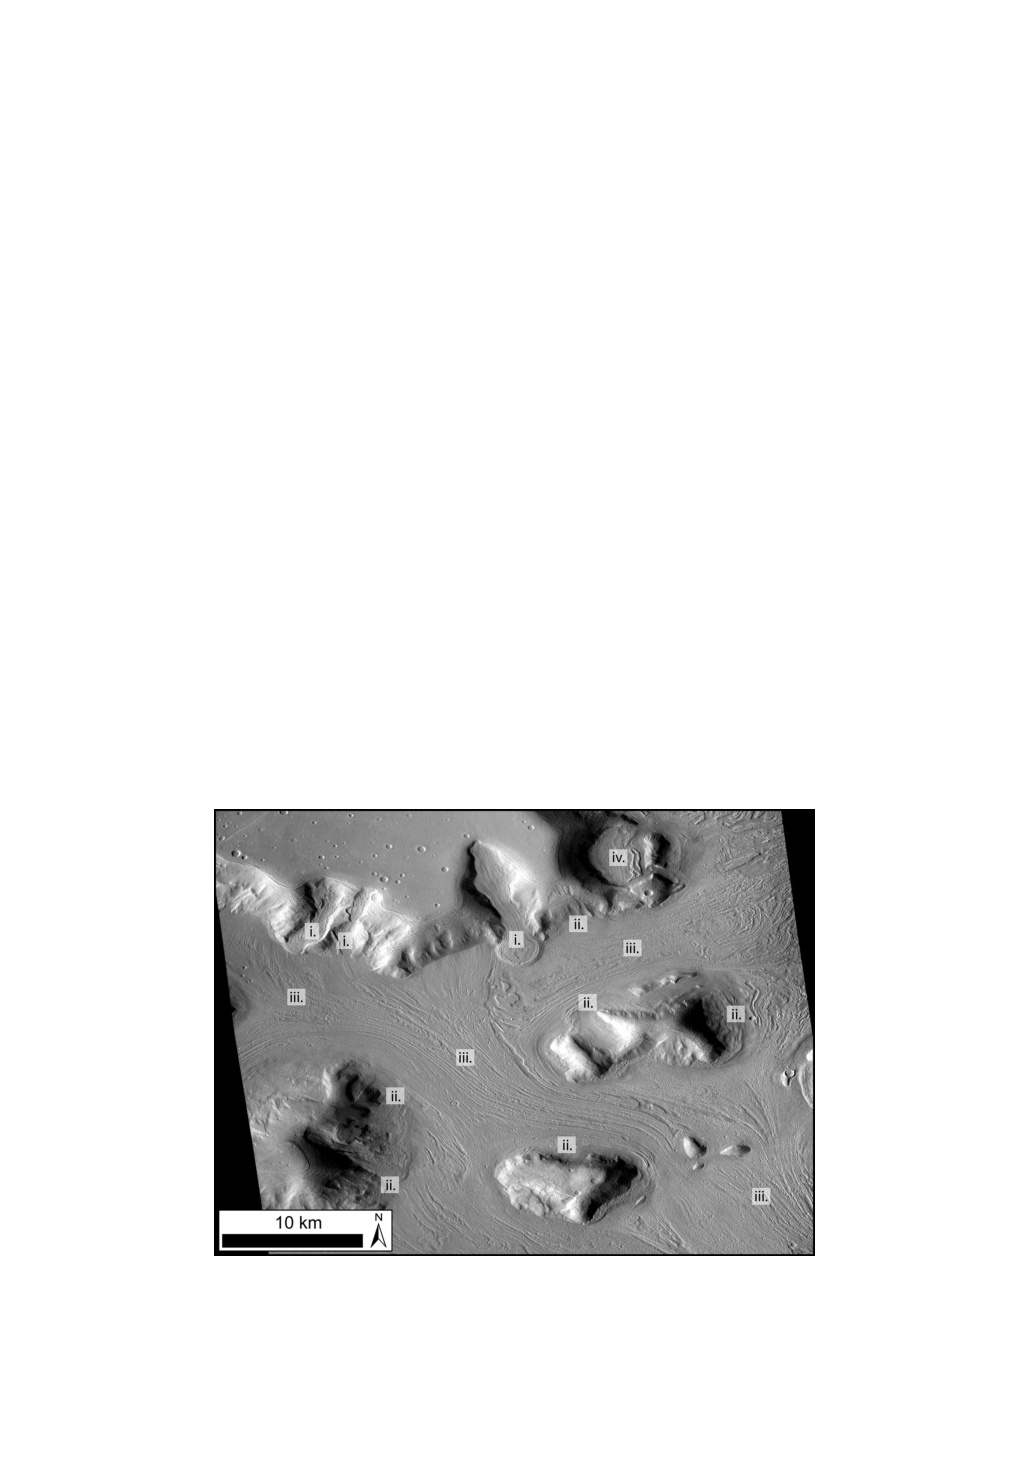
\includegraphics[
        width=\linewidth,
        height=0.65\textheight,
        keepaspectratio
    ]{Figures/Diagrams/Brough16_Fig1.pdf}
    \caption{CTX image data showing (i) GLFs; (ii) LDAs; (iii) LVFs; and (iv) CCFs at Protonilus Mensae ($42.62^{\circ}$N, $50.51^{\circ}$E; Figure from \cite{Brough16}).}
    \end{figure}
\end{frame}
\begin{frame}{Small-Scale Features}
    \begin{block}{Causes}
        \begin{itemize}
            \item Retreat of glacier
            \item Sublimation
            \item Fracture
            \item Exposure of underlying rock
        \end{itemize}
    \end{block}
\end{frame}

\begin{frame}{Small-Scale Features}
\begin{figure}
\centering
\begin{subfigure}{0.48\textwidth}
    \centering
    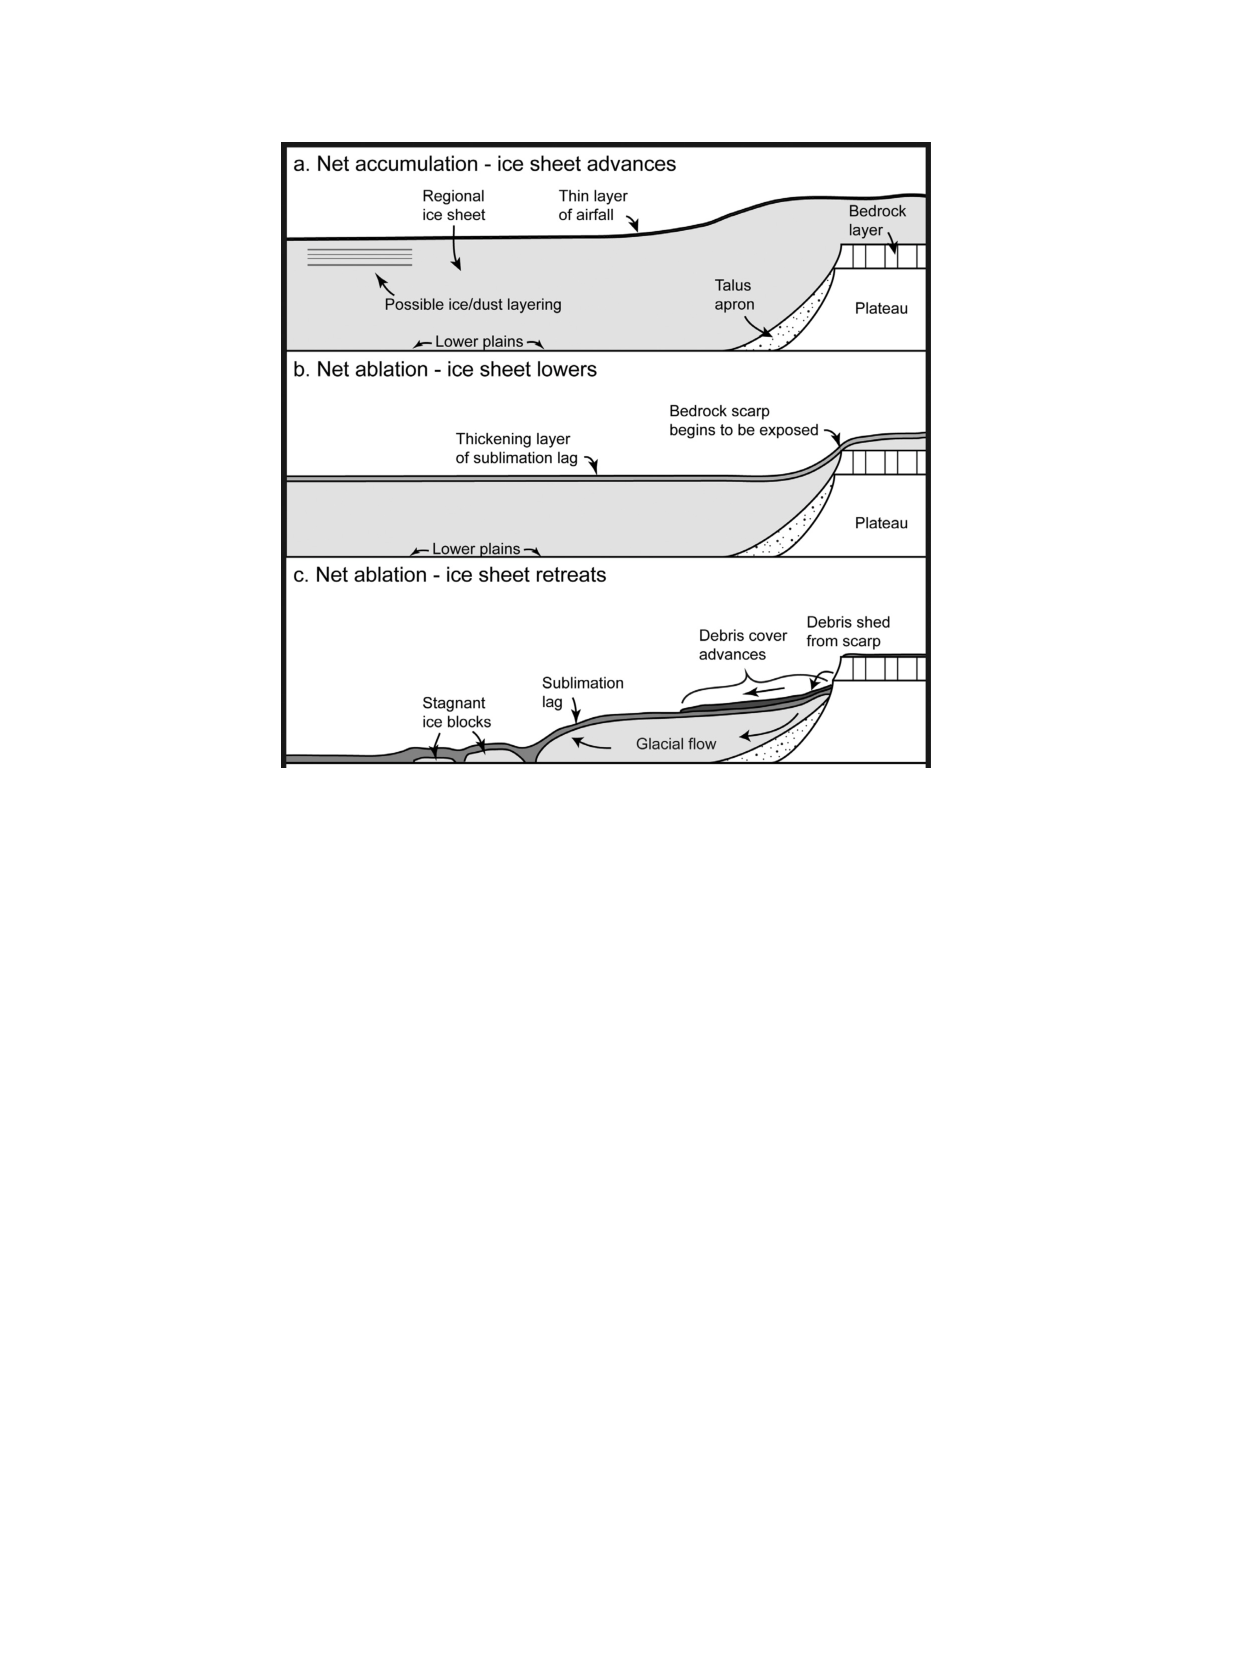
\includegraphics[
        width=\linewidth,
        height=0.65\textheight,
        keepaspectratio
    ]{Figures/Diagrams/Baker15_Fig17a.pdf}
\end{subfigure}
\hfill
\begin{subfigure}{0.48\textwidth}
    \centering
    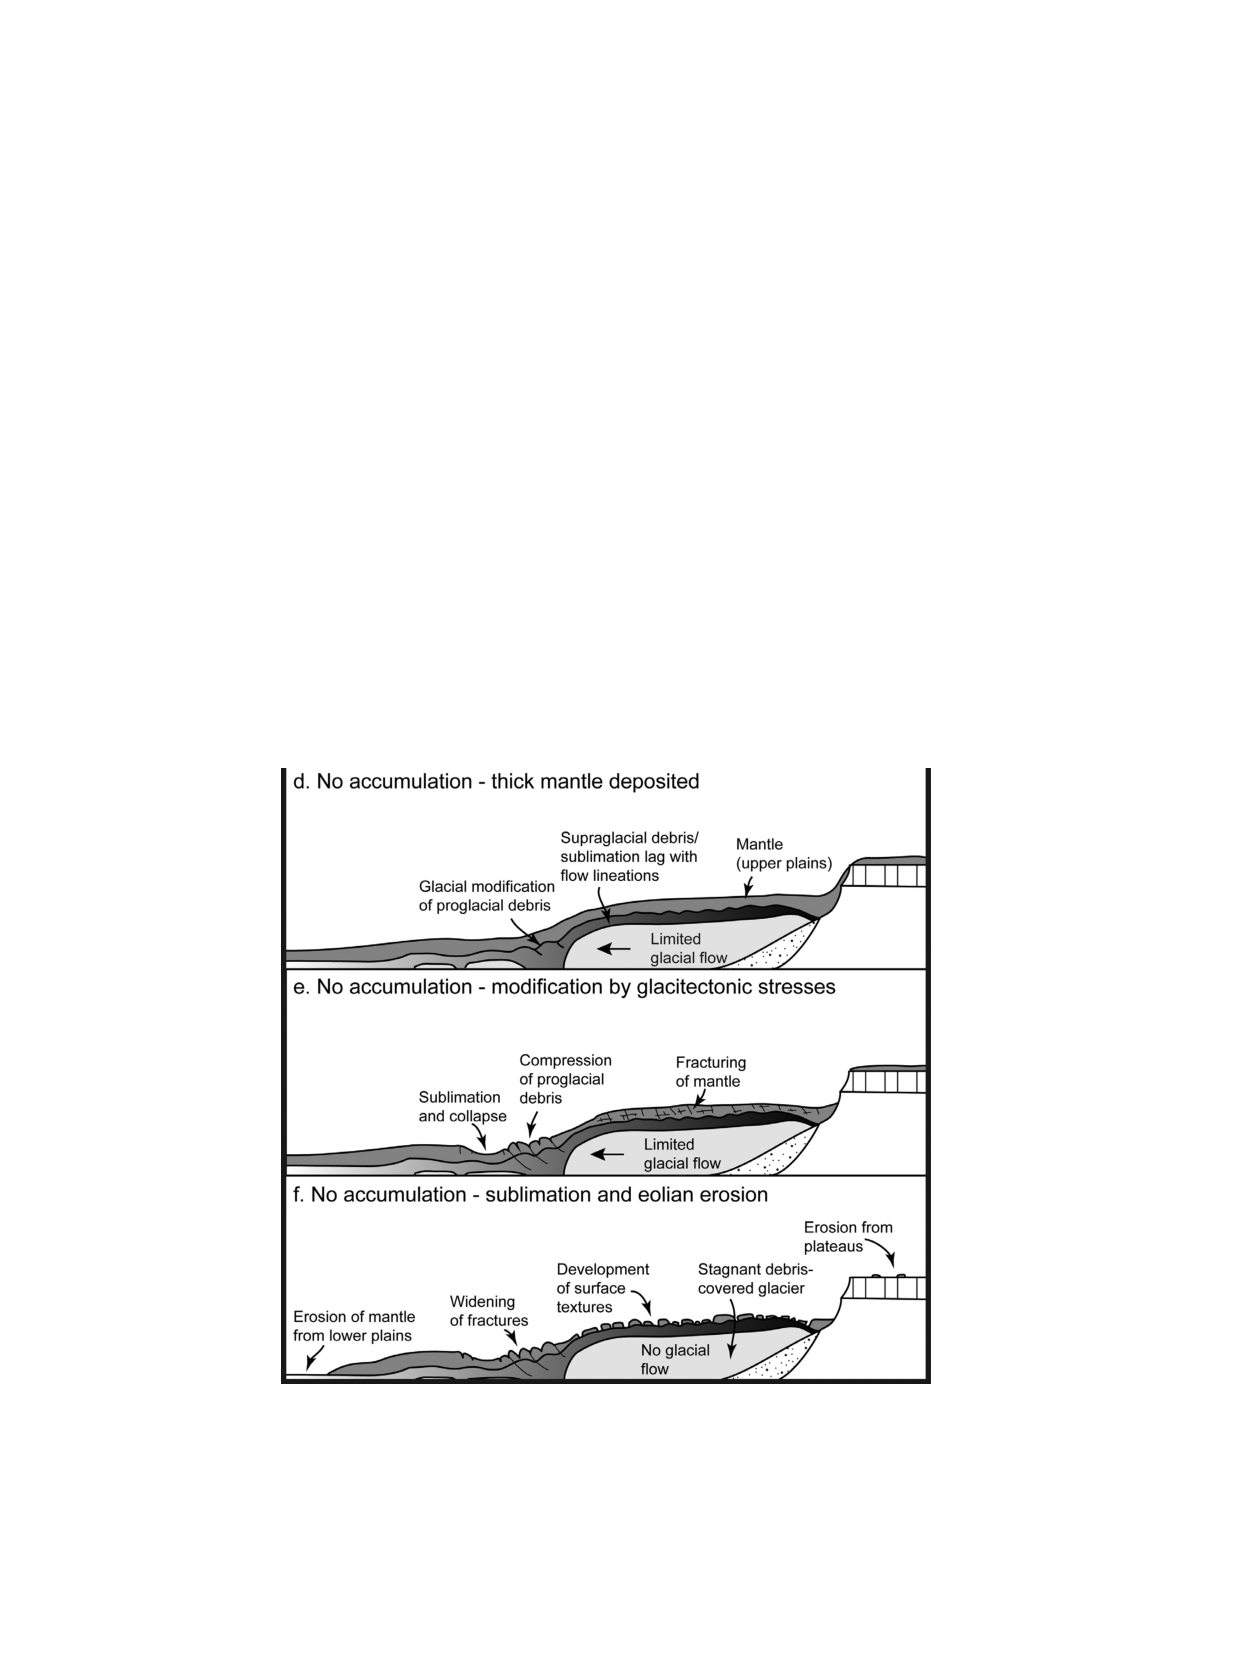
\includegraphics[
        width=\linewidth,
        height=0.65\textheight,
        keepaspectratio
    ]{Figures/Diagrams/Baker15_Fig17b.pdf}
\end{subfigure}
\caption{Schematic showing the mechanism of formation for glacier-related surface features (Figure from \cite{Baker15}).}
\label{fig:Baker15}

\end{figure}
\end{frame}
%%%%%%%%%%%%%%%%%%
\begin{frame}[label=RingMold]{Small-Scale Features: Craters}
\begin{figure}
    \centering
    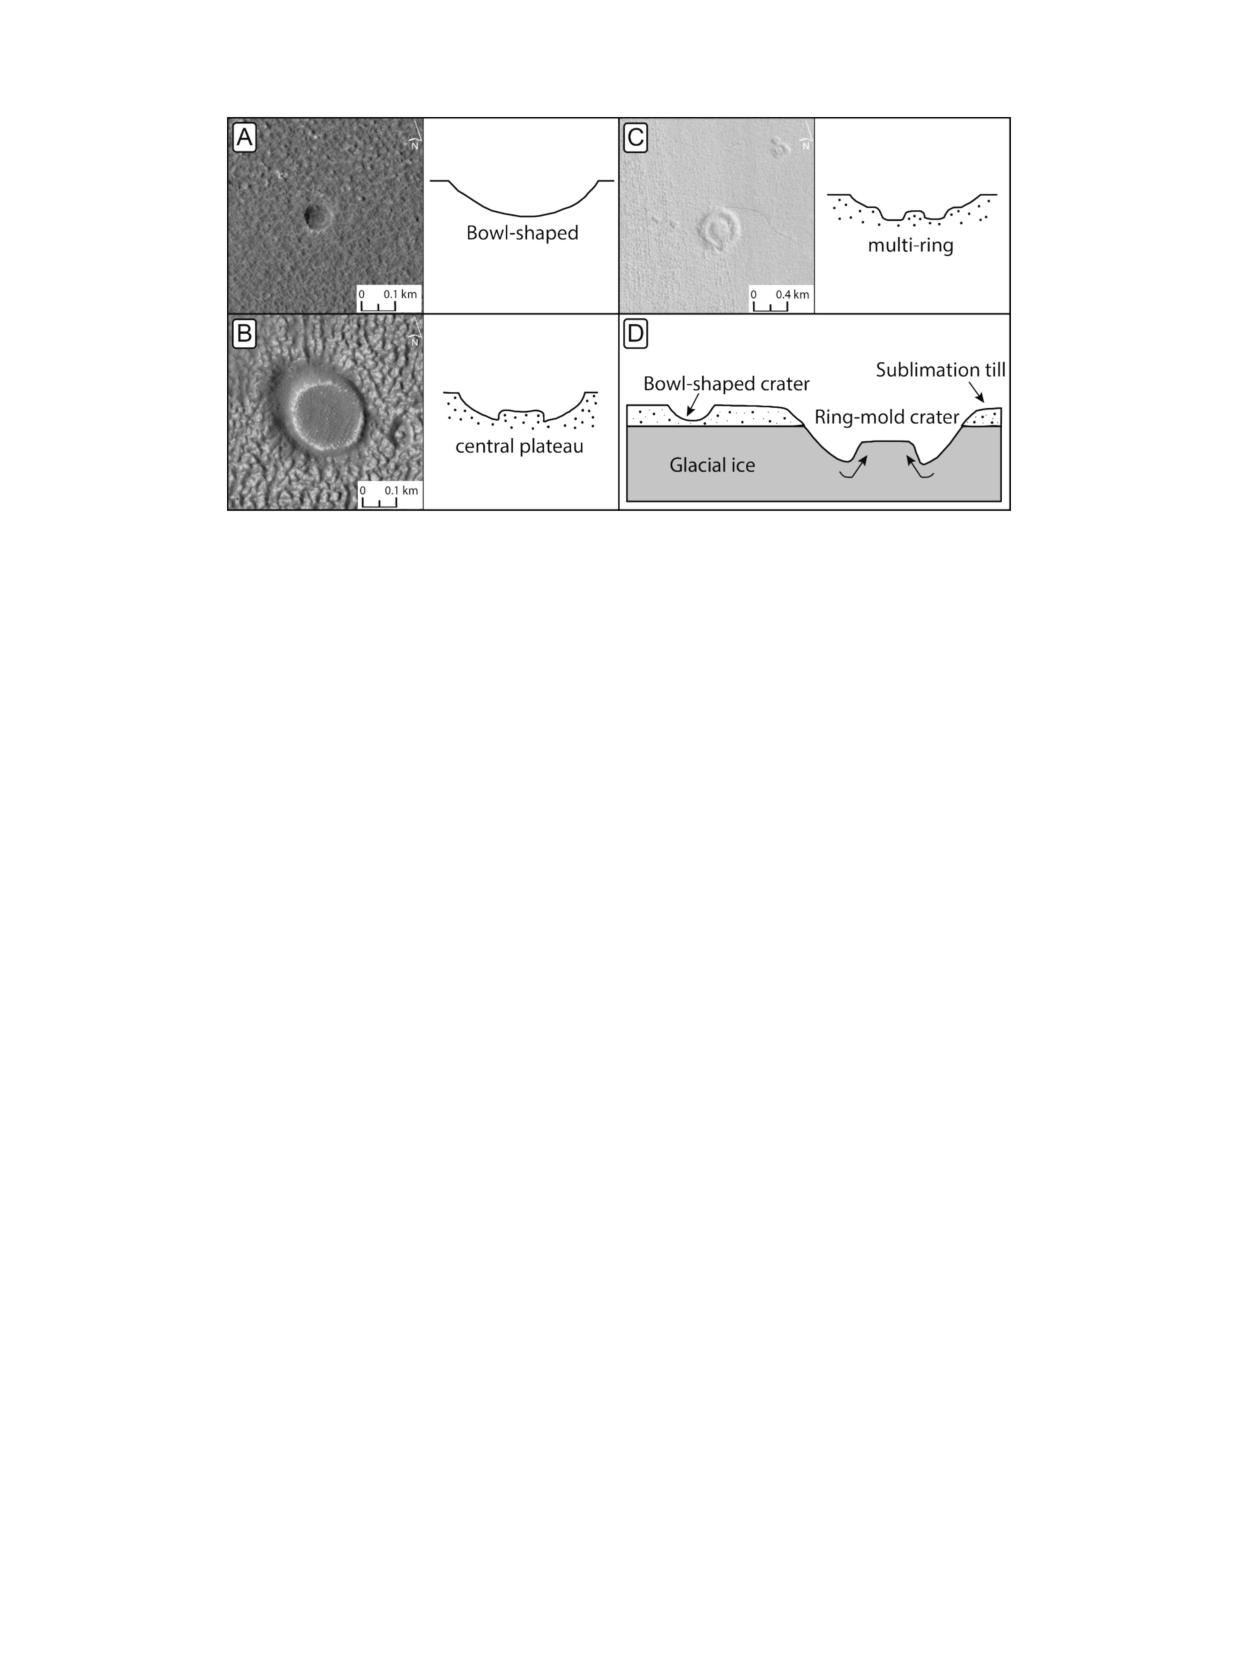
\includegraphics[
        width=\linewidth,
        height=0.65\textheight,
        keepaspectratio
    ]{Figures/Diagrams/Wueller25_Fig6.pdf}
    \caption{Diagram comparing the formation of bowl-shaped and ring-mold craters (Figure from \cite{Wueller25}).}
\label{fig:Wueller25_Fig6}
\end{figure}
\end{frame}
%%%%%%%%%%%%%%%%%%
\begin{frame}[label=SmallVFFs]{Small-Scale Features}
\begin{figure}
    \centering
    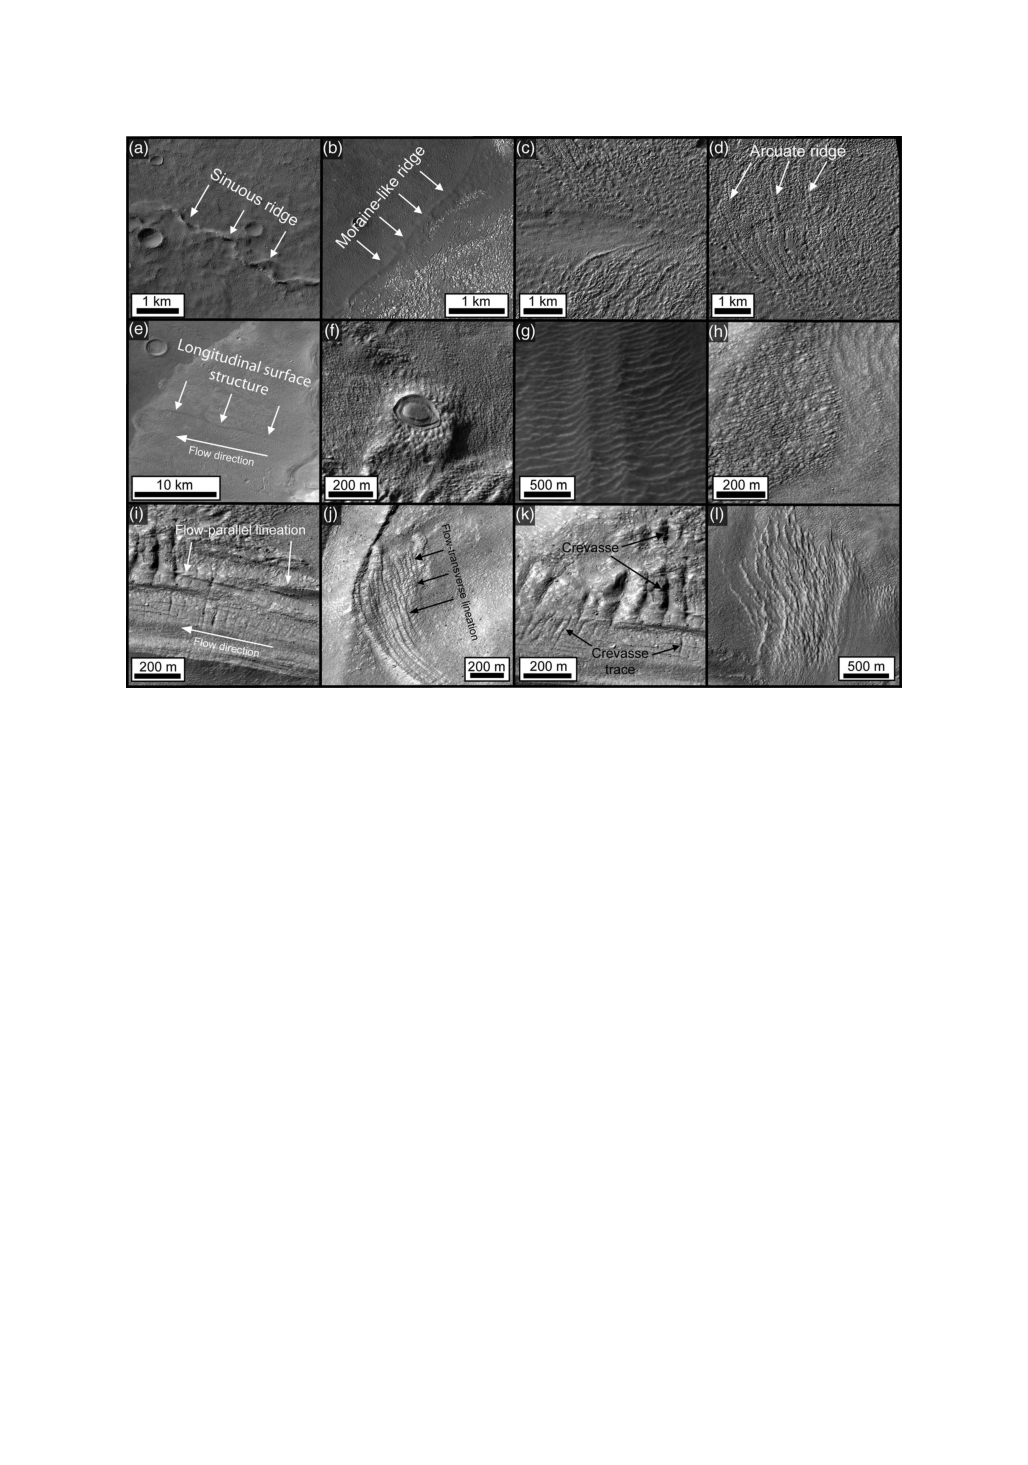
\includegraphics[
        width=\linewidth,
        height=0.65\textheight,
        keepaspectratio
    ]{Figures/Diagrams/Brough16_Fig3.pdf}
    \caption{Comparison between different surface features resulting from sublimation (Figure from \cite{Brough16}).}
    \label{fig:ButcherMangold_a}
\end{figure}
\end{frame}
\begin{frame}{GLF Example: Cirque (Corrie)}

    \begin{block}<+->{Identifying Features}
        \begin{itemize}
            \item Armchair shape
            \item At mountain or massif edge
            \item Two sidewalls
            \item Open downslope
        \end{itemize}
    \end{block}

    \begin{block}<+->{Similar Geomorphological Formations}
        \begin{itemize}
            \item Deep-seated landslide
            \item Amphitheatre-headed valley
        \end{itemize}
    \end{block}
        
    \begin{block}<+->{Mechanism of Alcove Formation}
        \begin{itemize}
            \item Glacial retreat and sublimation (cirque/corrie)
            \item Dry landslide (fractured rock...)
            \item Wet landslide (seepage erosion, saturated rock...)
        \end{itemize}
    \end{block}
\sidecite{(\cite{Li05,Guimper21,Li26})}
\end{frame}

\begin{frame}[label=Corrie]{GLF Example: Cirque (Corrie)}

\begin{figure}
\centering
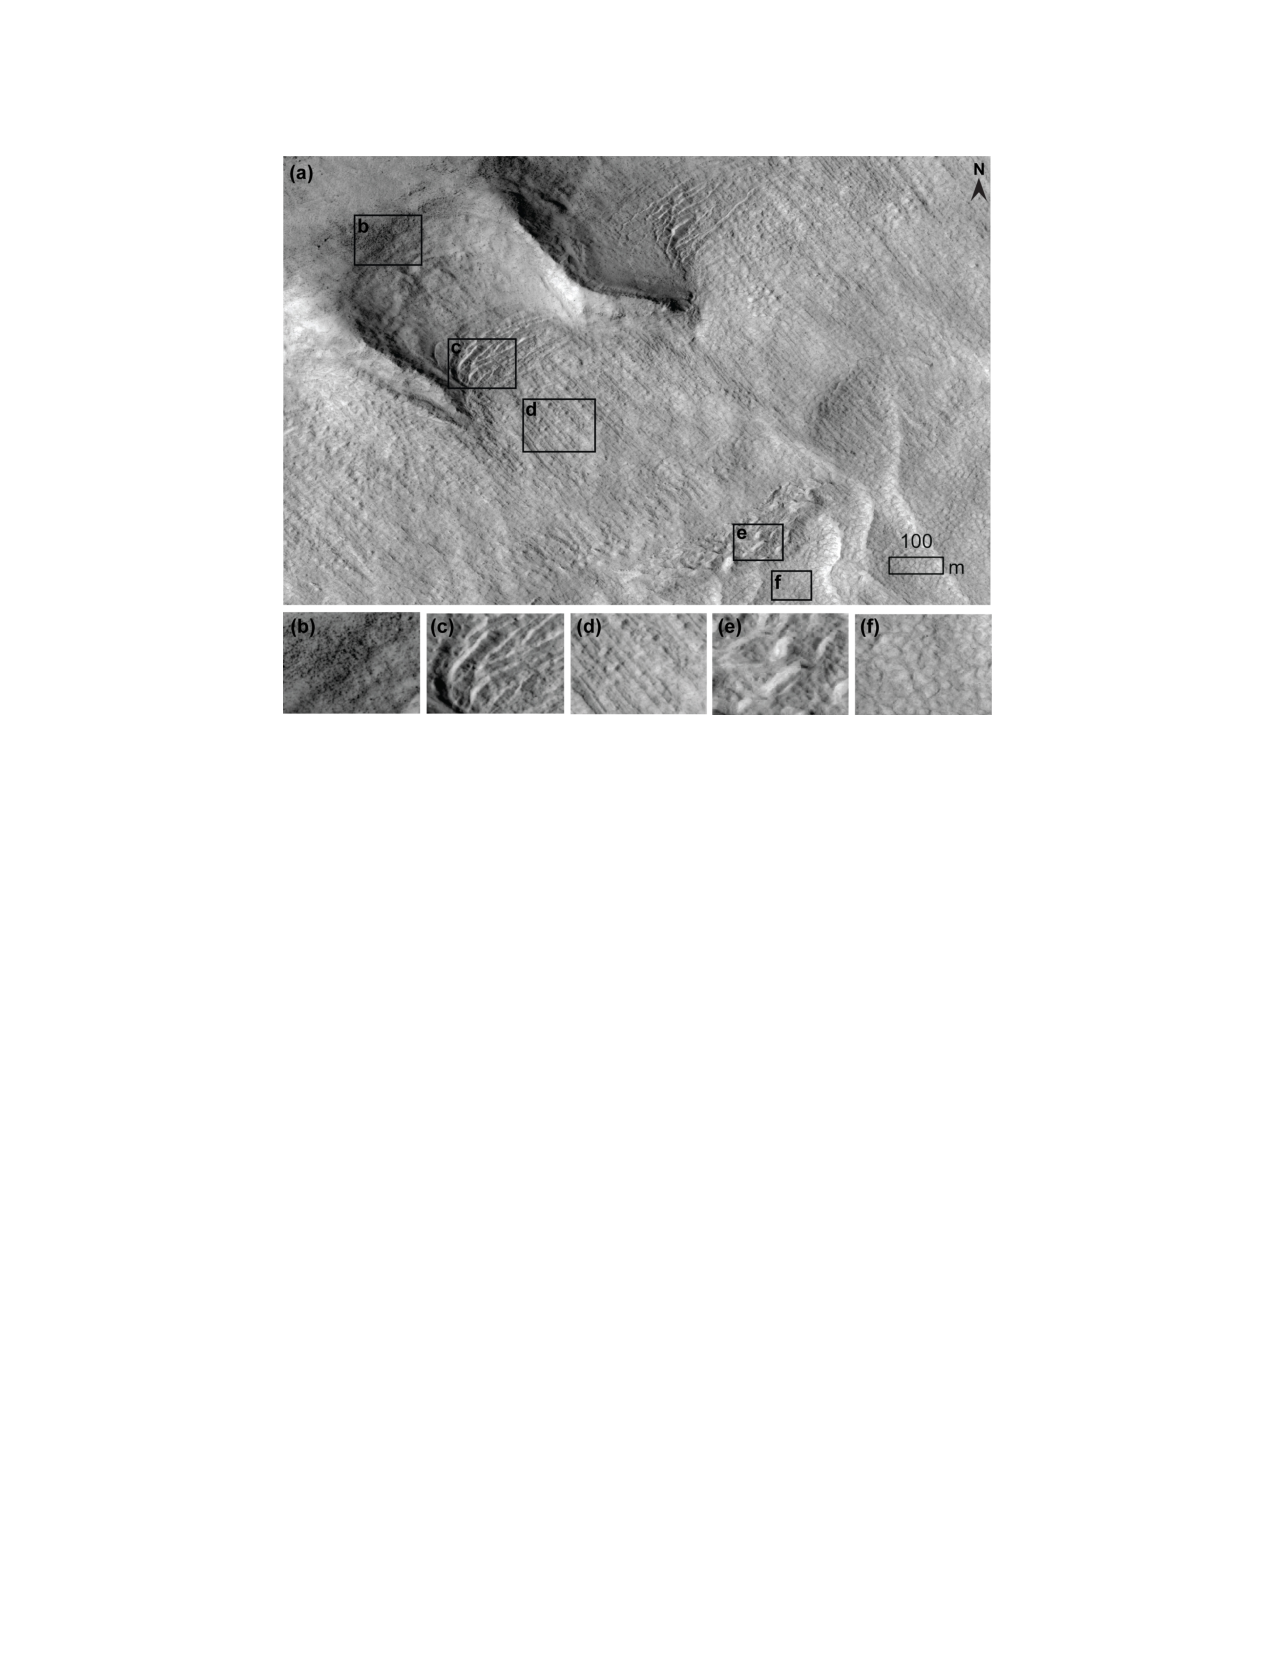
\includegraphics[
    height=0.6\textheight,
    keepaspectratio
]{Figures/Diagrams/Li26_Fig10.pdf}
\caption{HiRISE image data of a cirque-like alcove at Deuteronlius Mensae ($46.57^{\circ}$N, $22.12^{\circ}$E); (b) boulders at top of headwall; (c) washboard terrain; (d) linear terrain; (e) rectilinear ridges; (f) polygonal terrain (Figure from \cite{Li26}).}
\label{fig:Li26}
\end{figure}
\end{frame}

\begin{frame}{GLF Example: Cirque (Corrie)}
    \begin{figure}
    \centering
        \begin{subfigure}{0.48\linewidth}
            \centering
            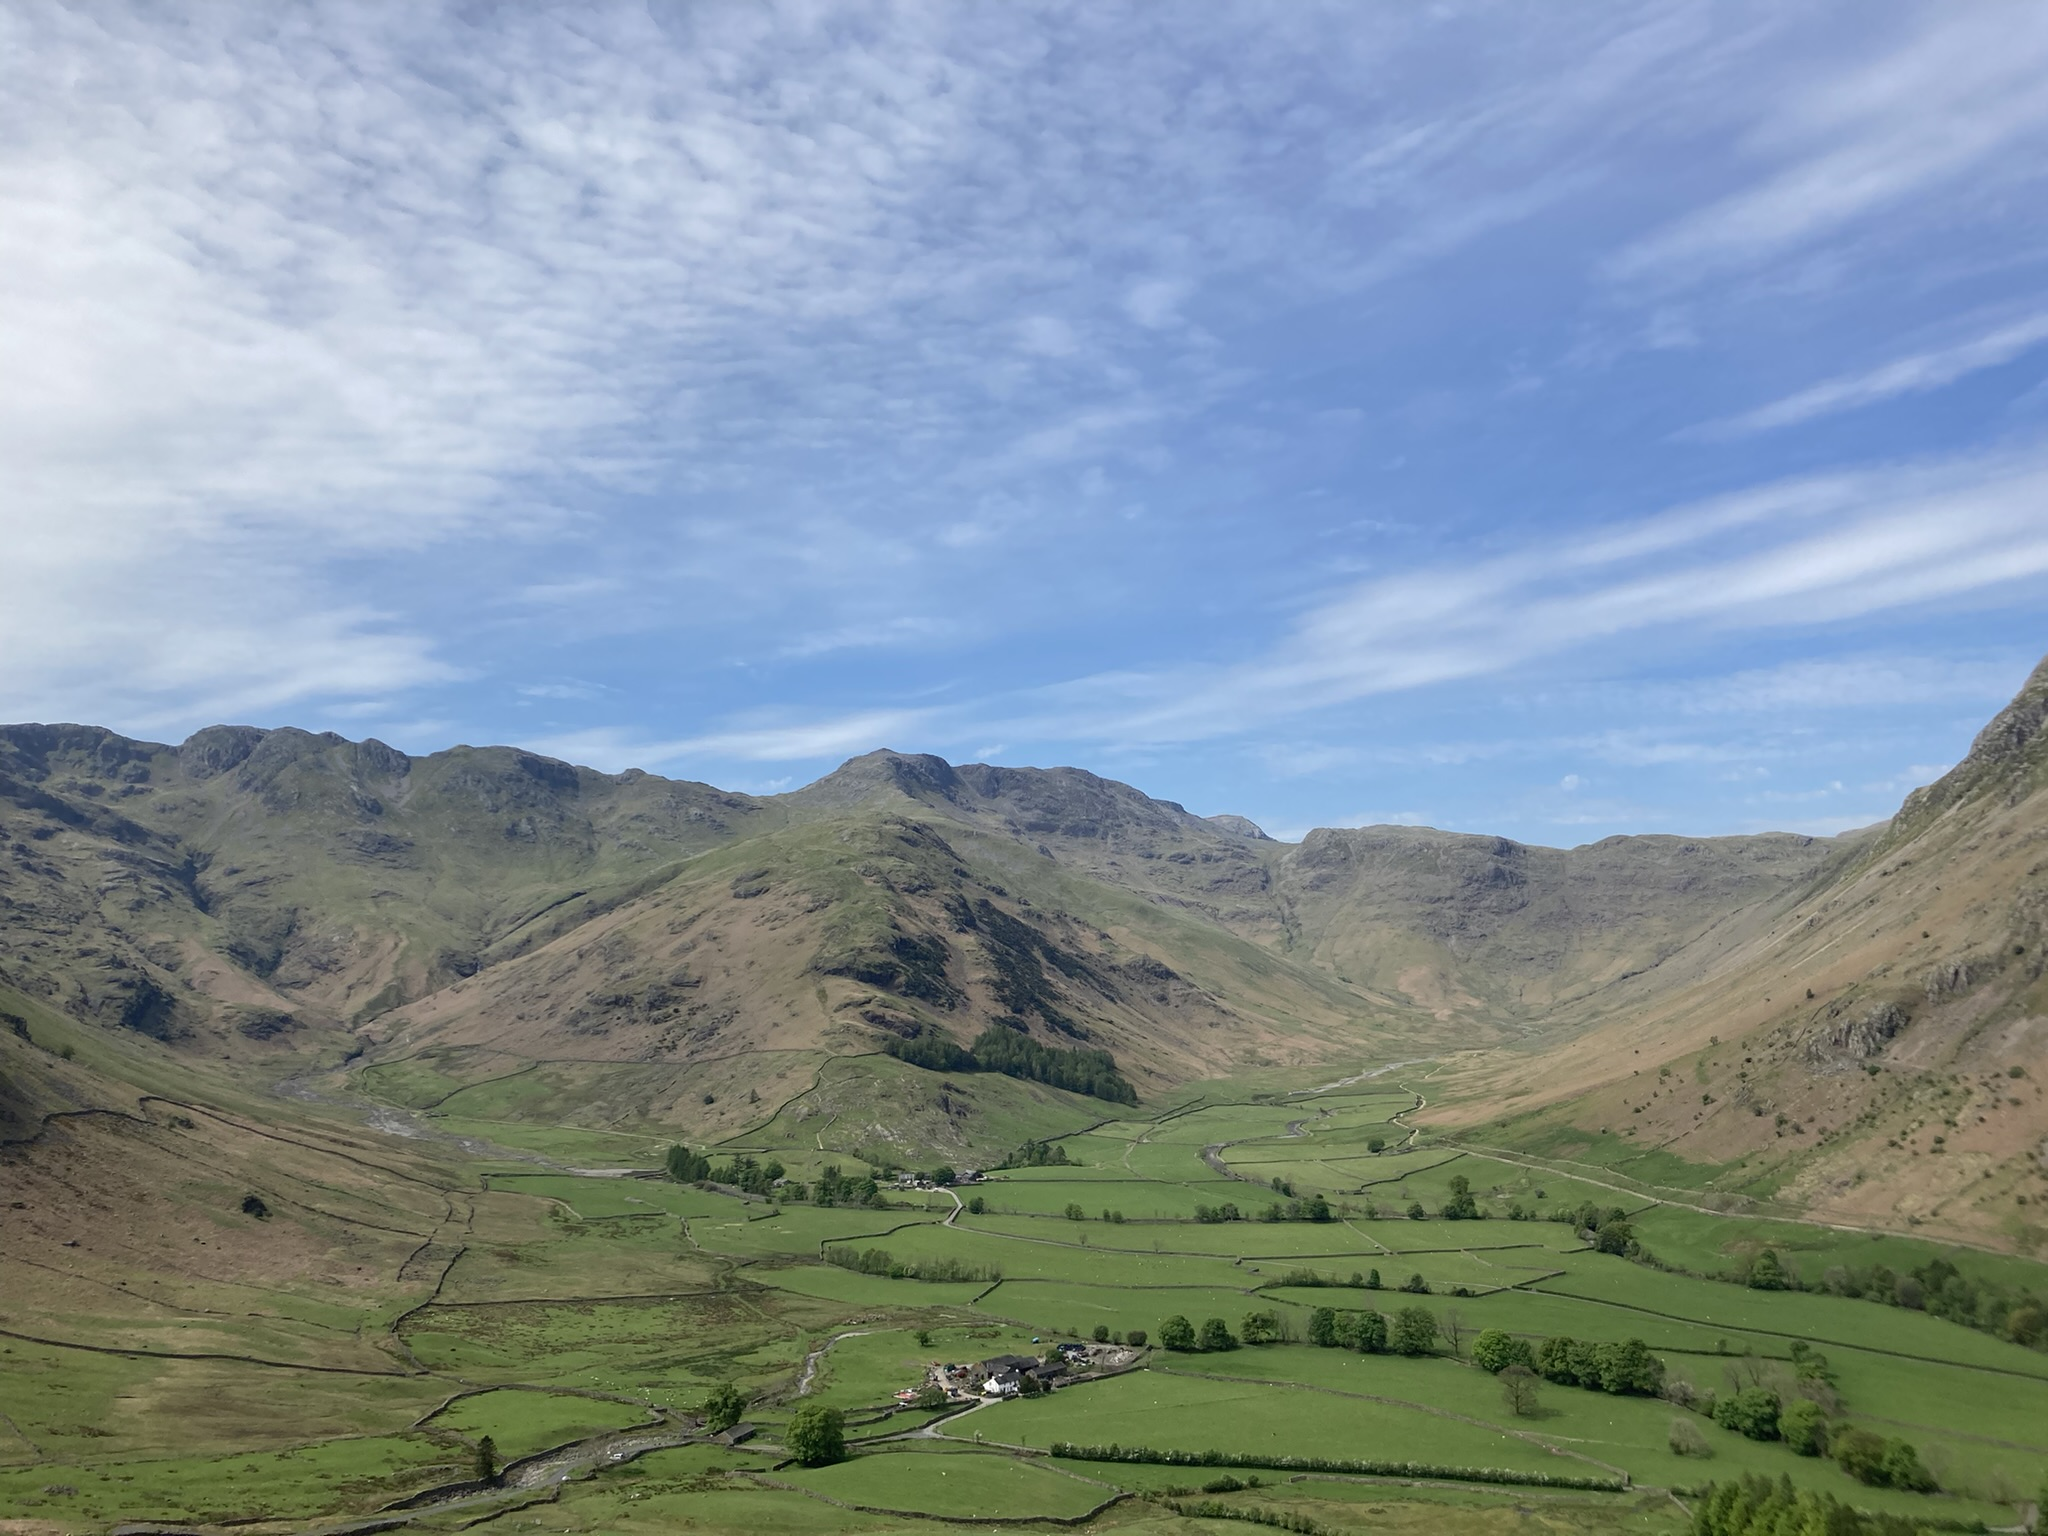
\includegraphics[width=\linewidth]{Figures/Corrie/Langdale_2.jpeg}
            \caption{View looking west from Great Langdale, toward Scafell Pike \(54.50^\circ\ \text{N}\) and \(-2.99^\circ\ \text{E}\).}
            \label{fig:Langdale_2}
        \end{subfigure}
        \hfill
        \begin{subfigure}{0.48\linewidth}
            \centering
            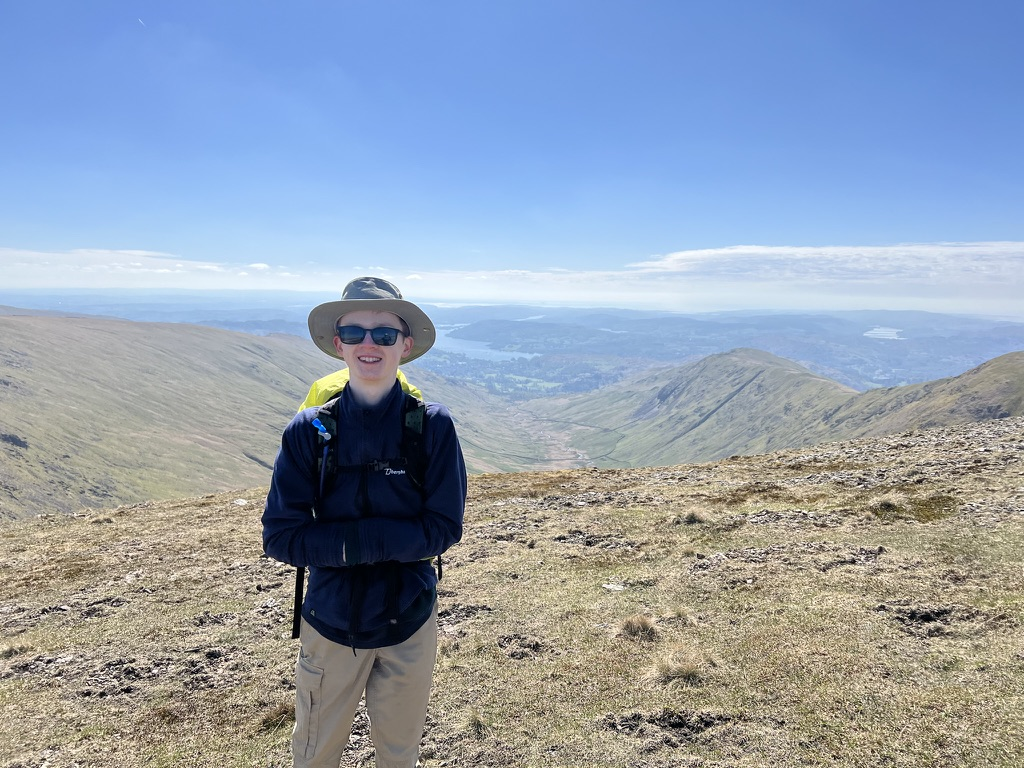
\includegraphics[width=\linewidth]{Figures/Corrie/Langdale_1.jpeg}
            \caption{View looking south from Fairfield over Deepdale.}
            \label{fig:Langdale_1}
        \end{subfigure}
        \caption{Views of corries at in the Lake District.}
        \label{fig:Langdale}
    \end{figure}
\end{frame}

%%%%%%%%%%%%%%%%%%%%%%%%%%%%%%%%%%%%%%
\section{Data}
\begin{frame}{Data: CTX}
    \begin{block}{CTX}
        \begin{itemize}
            \item Content Camera (CTX), Mars Reconnaissance Orbiter (MRO)
            \item Level 2
            \item B03\_010696\_2144\_XN\_34N343W
            \begin{itemize}
                \item Taken 2008-11-06 
                \item $\sim 5.90\ \mathrm{m\ px^{-1}}$ resolution
            \end{itemize}
            \item V23\_089052\_2140\_XN\_34N343W
            \begin{itemize}
                \item Taken 2025-07-26 
                \item $\sim 5.85\ \mathrm{m\ px^{-1}}$ resolution
                \item Processed at $1:100\ 000$ scale
            \end{itemize}
        \end{itemize}
    \end{block}
\end{frame}

\begin{frame}{Data: HRSC DEM}
    \begin{block}{HRSC}
        \begin{itemize}
            \item High Resolution Stereo Camera (HRSC), Mars Express
            \item Level 4
            \item h5267\_0000\_da4 (referenced to the GMM3 aeroid)
            \item Taken 2011-05-26
            \item $75\ \mathrm{m\ px^{-1}}$ resolution
            \item Processed at $1:100\ 000$ scale
        \end{itemize}
    \end{block}
\end{frame}

\begin{frame}{Data: HiRISE}
    \begin{block}{HiRISE}
        \begin{itemize}
            \item High Resolution Imaging Science Experiment (HiRISE), Mars Reconnaissance Orbiter (MRO)
            \item B\&W Map Projected
            \item ESP\_049187\_2150
            \item Taken 2017-01-23
            \item Sun incidence angle $62.1^{\circ}$
            \item $\sim 25\ \mathrm{cm\ px^{-1}}$ resolution
            \item Processed at $1:2\ 000$ scale
        \end{itemize}
    \end{block}
\end{frame}
%%%%%%%%%%%%%%%%%%%%%%%%%%%%%%%%%%%%%%
\section{Overview of NW Ismenius Cavus}
%%%%%%%%%%%%%%%%%%%%%%%%%%%%%%%%%%%%%%
\begin{frame}[label=RegionalMap]{Regional Map}

\begin{figure}
\centering

\begin{subfigure}{0.48\textwidth}
    \centering
    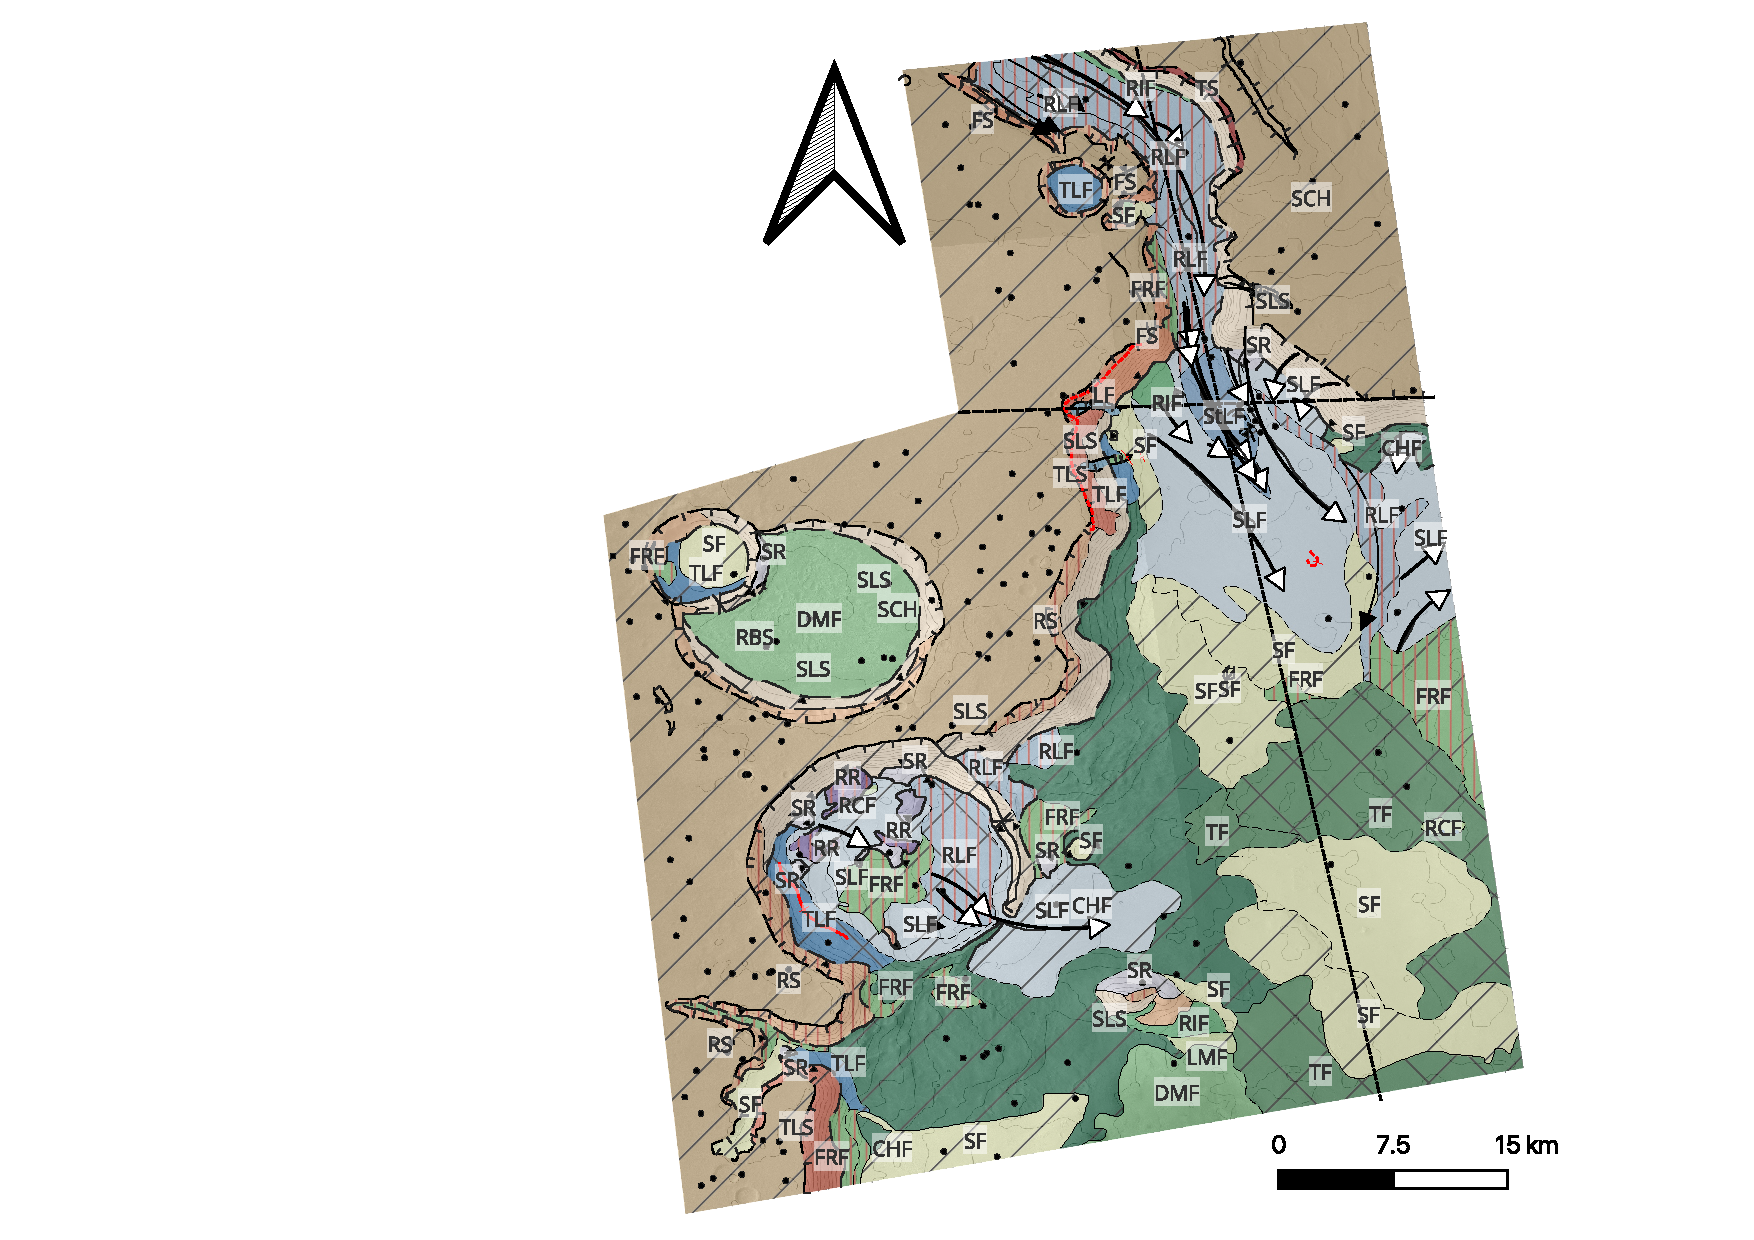
\includegraphics[
        width=\linewidth,
        height=0.65\textheight,
        keepaspectratio
    ]{Figures/Maps/CTX_Map.pdf}
    \label{fig:CTXOverview_a}
\end{subfigure}
\hfill
\begin{subfigure}{0.48\textwidth}
    \centering
    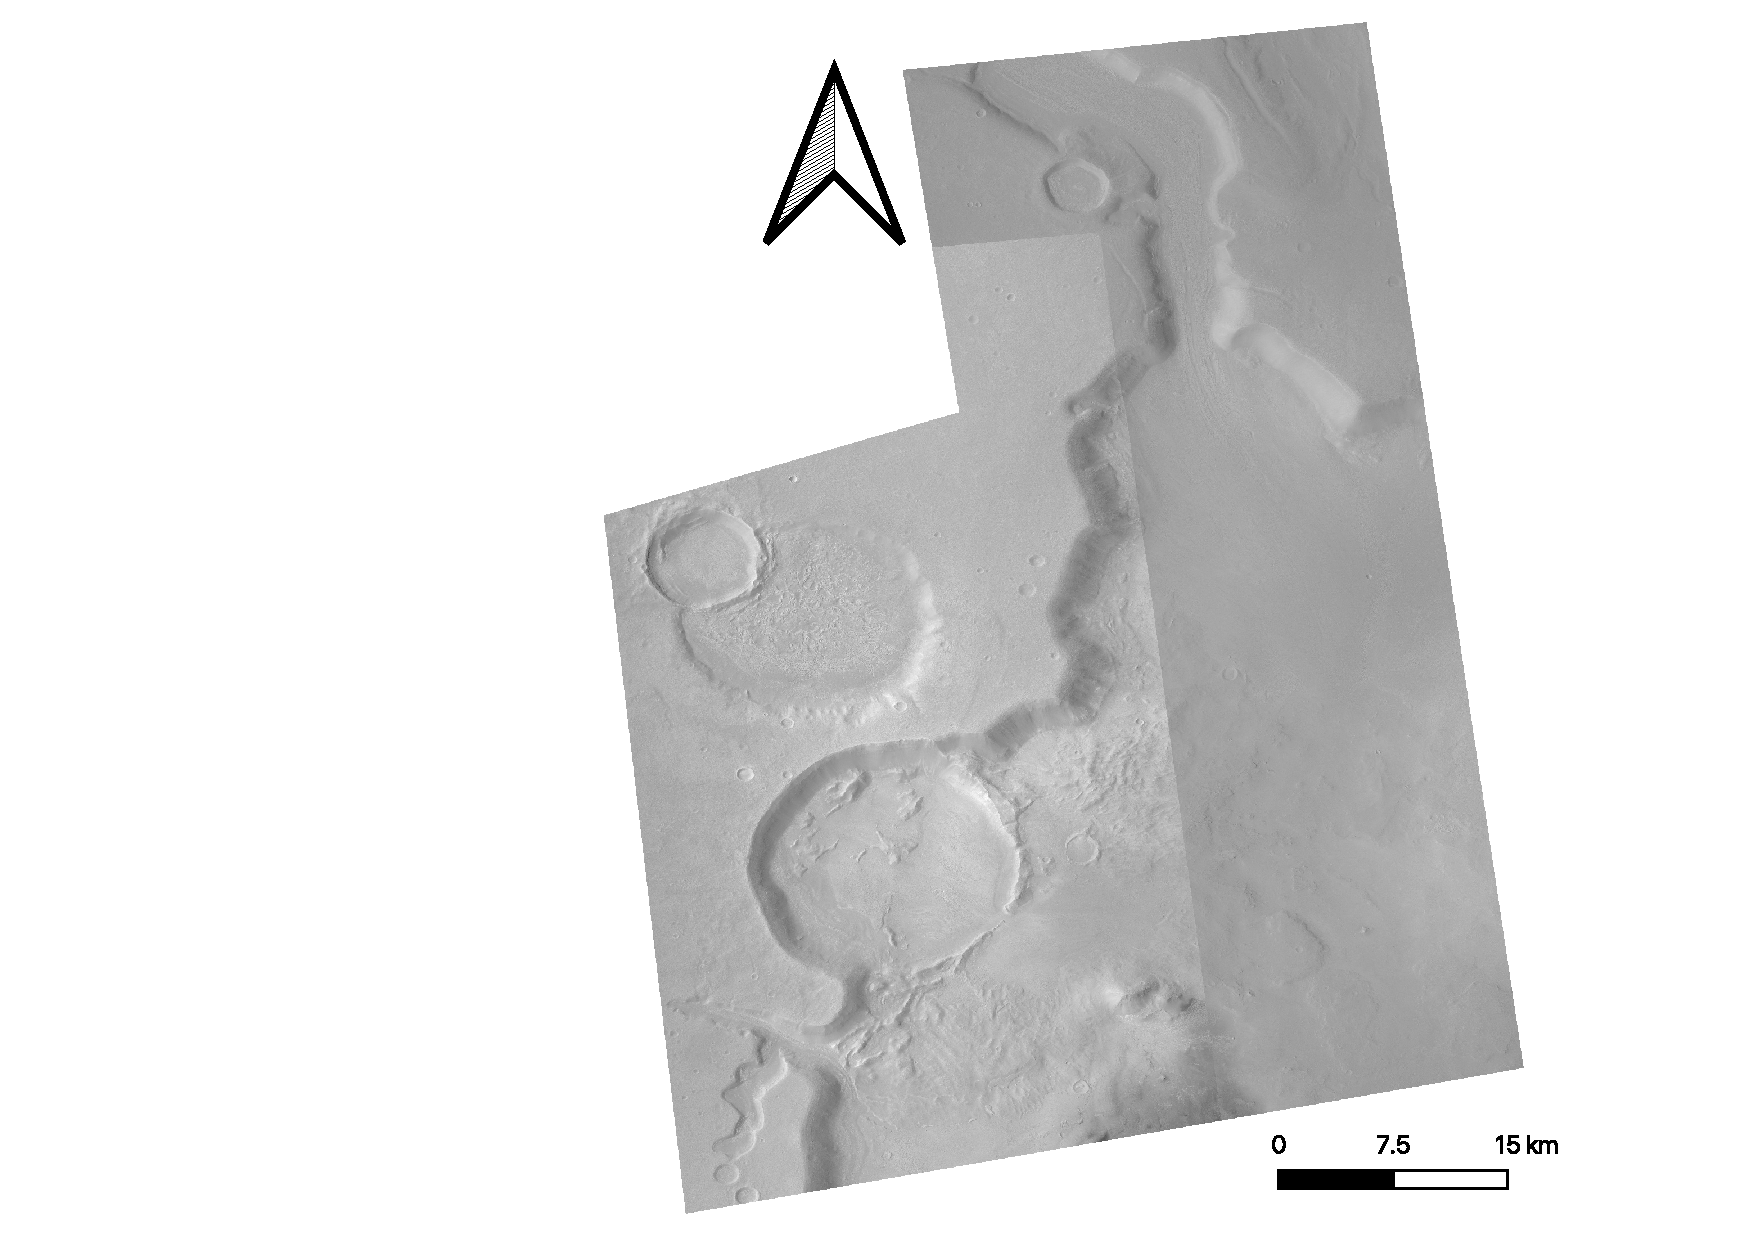
\includegraphics[
        width=\linewidth,
        height=0.65\textheight,
        keepaspectratio
    ]{Figures/Maps/CTX_Img.pdf}
    \label{fig:CTXOverview_b}
\end{subfigure}

\caption{Overview of NW Ismenius Cavus, mapped using CTX and the HRSC DEM data ($1:100\ 000$ scale). Craters identified using YOLOLens (\cite{LaGrassa}).}
\label{fig:CTXOverview}

\end{figure}

\end{frame}


\begin{frame}{Map Patterns}

\centering

\definecolor{rubbleblue}{HTML}{377EB8}

\begin{tikzpicture}[x=1cm,y=1cm]

% \node[font=\Large] at (4.5,0)
% {Surface Texture Patterns};

%--------------------------------------------------
% DEGRADED
%--------------------------------------------------

\fill[white]
(0,-1.4) rectangle (1,-0.4);

\draw[
pattern=north east lines
]
(0,-1.4) rectangle (1,-0.4);

\draw
(0,-1.4) rectangle (1,-0.4);

\node[
anchor=west,
font=\large
]
at (1.4,-0.9)
{Degraded};

%--------------------------------------------------
% HIGHLY DEGRADED
%--------------------------------------------------

\fill[white]
(0,-3.0) rectangle (1,-2.0);

\draw[
pattern=crosshatch
]
(0,-3.0) rectangle (1,-2.0);

\draw
(0,-3.0) rectangle (1,-2.0);

\node[
anchor=west,
font=\large
]
at (1.4,-2.5)
{Highly degraded};

%--------------------------------------------------
% ROUGH
%--------------------------------------------------

\fill[white]
(0,-4.6) rectangle (1,-3.6);

\foreach \x in {0.10,0.30,0.50,0.70,0.90}
{
    \draw[
    red,
    line width=0.4pt
    ]
    (\x,-4.6)--(\x,-3.6);
}

\draw
(0,-4.6) rectangle (1,-3.6);

\node[
anchor=west,
font=\large
]
at (1.4,-4.1)
{Rough};

%--------------------------------------------------
% RUBBLE
%--------------------------------------------------

\fill[white]
(0,-6.2) rectangle (1,-5.2);

% top row

\foreach \x in {0.15,0.45,0.75}
{
    \fill[rubbleblue]
    (\x,-5.35)
    circle (0.035);
}

% second row

\foreach \x in {0.30,0.60,0.90}
{
    \fill[rubbleblue]
    (\x,-5.55)
    circle (0.035);
}

% third row

\foreach \x in {0.15,0.45,0.75}
{
    \fill[rubbleblue]
    (\x,-5.75)
    circle (0.035);
}

% fourth row

\foreach \x in {0.30,0.60,0.90}
{
    \fill[rubbleblue]
    (\x,-5.95)
    circle (0.035);
}

% fifth row

\foreach \x in {0.15,0.45,0.75}
{
    \fill[rubbleblue]
    (\x,-6.15)
    circle (0.035);
}

\draw
(0,-6.2) rectangle (1,-5.2);

\node[
anchor=west,
font=\large
]
at (1.4,-5.7)
{Rubble};

\end{tikzpicture}

\end{frame}
\begin{frame}{Lineations and Boundaries}

\centering

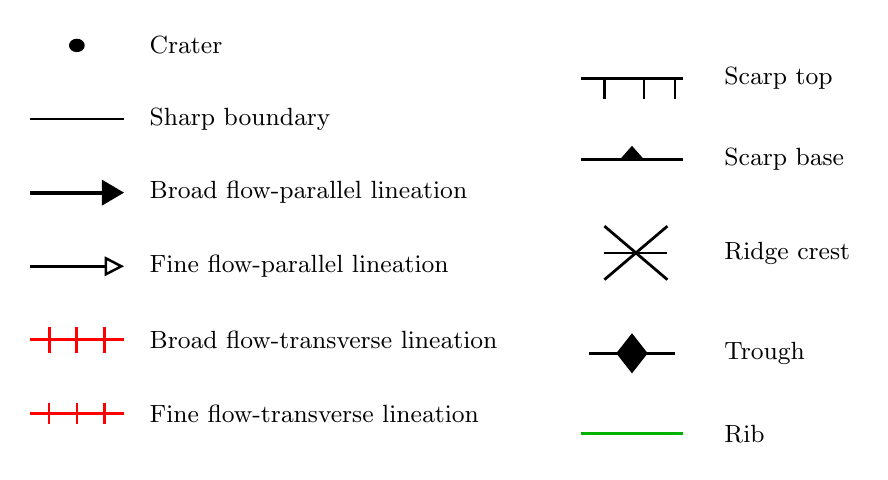
\begin{tikzpicture}[x=1cm,y=0.85cm]

%=================================================
% LEFT COLUMN
%=================================================

% Crater

\fill (0.6,-0.5) circle (0.10);

\node[anchor=west,font=\small]
at (1.4,-0.5)
{Crater};

% Sharp boundary

\draw[line width=1pt]
(0,-1.6)--(1.2,-1.6);

\node[anchor=west,font=\small]
at (1.4,-1.6)
{Sharp boundary};

% Broad flow-parallel

\draw[
-{Triangle[length=8pt,width=9pt]},
line width=1.4pt
]
(0,-2.7)--(1.2,-2.7);

\node[anchor=west,font=\small]
at (1.4,-2.7)
{Broad flow-parallel lineation};

% Fine flow-parallel

\draw[
-{Triangle[length=7pt,width=7pt,open]},
line width=0.9pt
]
(0,-3.8)--(1.2,-3.8);

\node[anchor=west,font=\small]
at (1.4,-3.8)
{Fine flow-parallel lineation};

% Broad flow-transverse

\draw[red,line width=1.1pt]
(0,-4.9)--(1.2,-4.9);

\foreach \x in {0.25,0.60,0.95}
{
\draw[red,line width=1.1pt]
(\x,-5.1)--(\x,-4.7);
}

\node[anchor=west,font=\small]
at (1.4,-4.9)
{Broad flow-transverse lineation};

% Fine flow-transverse

\draw[red,line width=0.8pt]
(0,-6.0)--(1.2,-6.0);

\foreach \x in {0.25,0.60,0.95}
{
\draw[red,line width=0.8pt]
(\x,-6.15)--(\x,-5.85);
}

\node[anchor=west,font=\small]
at (1.4,-6.0)
{Fine flow-transverse lineation};

%=================================================
% RIGHT COLUMN
%=================================================

% Scarp top

\draw[line width=1pt]
(7.0,-1.0)--(8.3,-1.0);

\foreach \x in {7.3,7.8,8.2}
{
\draw[line width=0.8pt]
(\x,-1.0)--(\x,-1.3);
}

\node[anchor=west,font=\small]
at (8.7,-1.0)
{Scarp top};

% Scarp base

\draw[line width=1pt]
(7.0,-2.2)--(8.3,-2.2);

\fill
(7.65,-2.0)--(7.50,-2.2)--(7.80,-2.2)--cycle;

\node[anchor=west,font=\small]
at (8.7,-2.2)
{Scarp base};

% Ridge crest

\draw[line width=1pt]
(7.3,-3.6)--(8.1,-3.6);

\draw[line width=1pt]
(7.3,-4.0)--(8.1,-3.2);

\draw[line width=1pt]
(7.3,-3.2)--(8.1,-4.0);

\node[anchor=west,font=\small]
at (8.7,-3.6)
{Ridge crest};

% Trough

\draw[line width=1pt]
(7.1,-5.1)--(8.2,-5.1);

\fill
(7.65,-4.8)--(7.45,-5.1)--(7.85,-5.1)--cycle;

\fill
(7.65,-5.4)--(7.45,-5.1)--(7.85,-5.1)--cycle;

\node[anchor=west,font=\small]
at (8.7,-5.1)
{Trough};

% Rib

\draw[green!70!black,line width=1.3pt]
(7.0,-6.3)--(8.3,-6.3);

\node[anchor=west,font=\small]
at (8.7,-6.3)
{Rib};

\end{tikzpicture}

\end{frame}

%%%%%%%%

\begin{frame}{Lineations and Boundaries: Gradational / Degraded}

\centering

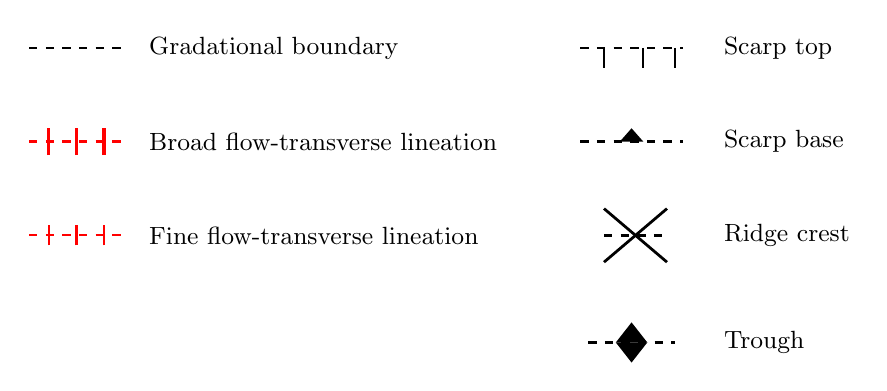
\begin{tikzpicture}[x=1cm,y=0.85cm]

%=================================================
% LEFT COLUMN
%=================================================

% Gradational boundary

\draw[dashed,line width=1pt]
(0,-1.0)--(1.2,-1.0);

\node[anchor=west,font=\small]
at (1.4,-1.0)
{Gradational boundary};

%  broad flow-transverse

\draw[red,dashed,line width=1.1pt]
(0,-2.4)--(1.2,-2.4);

\foreach \x in {0.25,0.60,0.95}
{
\draw[red,line width=1.1pt]
(\x,-2.6)--(\x,-2.2);
}

\node[anchor=west,font=\small]
at (1.4,-2.4)
{ Broad flow-transverse lineation};

%  fine flow-transverse

\draw[red,dashed,line width=0.8pt]
(0,-3.8)--(1.2,-3.8);

\foreach \x in {0.25,0.60,0.95}
{
\draw[red,line width=0.8pt]
(\x,-3.95)--(\x,-3.65);
}

\node[anchor=west,font=\small]
at (1.4,-3.8)
{ Fine flow-transverse lineation};

%=================================================
% RIGHT COLUMN
%=================================================

%  Scarp top

\draw[dashed,line width=1pt]
(7.0,-1.0)--(8.3,-1.0);

\foreach \x in {7.3,7.8,8.2}
{
\draw[line width=0.8pt]
(\x,-1.0)--(\x,-1.3);
}

\node[anchor=west,font=\small]
at (8.7,-1.0)
{ Scarp top};

%  Scarp base

\draw[dashed,line width=1pt]
(7.0,-2.4)--(8.3,-2.4);

\fill
(7.65,-2.2)--(7.50,-2.4)--(7.80,-2.4)--cycle;

\node[anchor=west,font=\small]
at (8.7,-2.4)
{ Scarp base};


% Ridge crest
\draw[dashed,line width=1pt]
(7.3,-3.8)--(8.1,-3.8);
\draw[line width=1pt]
(7.3,-4.2)--(8.1,-3.4);
\draw[line width=1pt]
(7.3,-3.4)--(8.1,-4.2);
\node[anchor=west,font=\small]
at (8.7,-3.8)
{ Ridge crest};

%  Trough

\draw[dashed,line width=1pt]
(7.1,-5.4)--(8.2,-5.4);

\fill
(7.65,-5.1)--(7.45,-5.4)--(7.85,-5.4)--cycle;

\fill
(7.65,-5.7)--(7.45,-5.4)--(7.85,-5.4)--cycle;

\node[anchor=west,font=\small]
at (8.7,-5.4)
{ Trough};

\end{tikzpicture}

\end{frame}
\begin{frame}{Regional Map Legend}

\centering

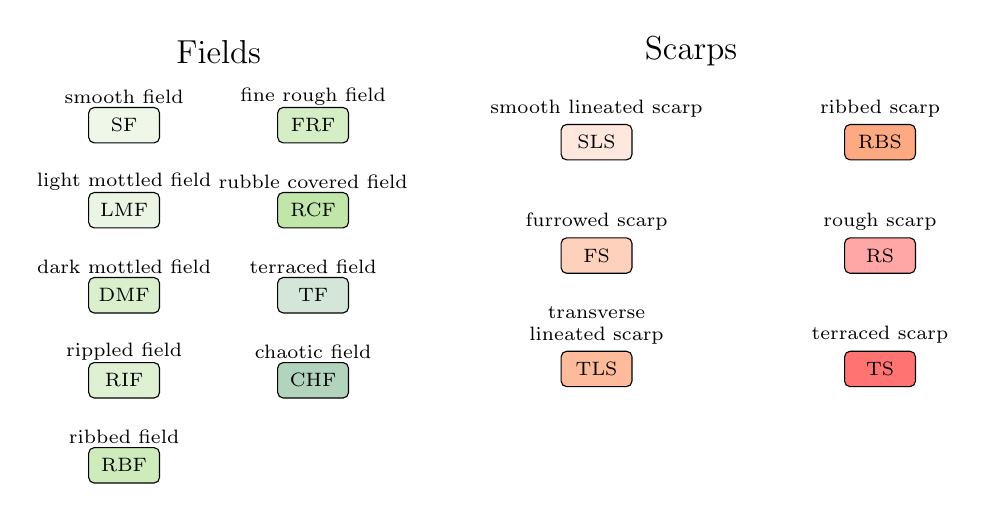
\begin{tikzpicture}[x=2.4cm,y=0.72cm]  % <-- reduced y scale

\tikzset{
legendunit/.style={
draw=black,
rounded corners=2pt,
minimum width=0.9cm,
minimum height=0.45cm,
font=\scriptsize
},
legendlabel/.style={
align=center,
font=\scriptsize
}
}

%----------------------------------
% HEADERS
%----------------------------------

\node[font=\large] at (0,0) {Fields};
\node[font=\large] at (2.5,0) {Scarps};

%----------------------------------
% FIELDS COLUMN 1
%----------------------------------

\node[legendlabel] at (-0.5,-0.8) {smooth field};
\node[legendunit,fill=fieldgreen!20] at (-0.5,-1.3) {SF};

\node[legendlabel] at (-0.5,-2.3) {light mottled field};
\node[legendunit,fill=fieldgreen!25] at (-0.5,-2.8) {LMF};

\node[legendlabel] at (-0.5,-3.8) {dark mottled field};
\node[legendunit,fill=fieldgreen!45] at (-0.5,-4.3) {DMF};

\node[legendlabel] at (-0.5,-5.3) {rippled field};
\node[legendunit,fill=fieldgreen!40] at (-0.5,-5.8) {RIF};

\node[legendlabel] at (-0.5,-6.8) {ribbed field};
\node[legendunit,fill=fieldgreen!60] at (-0.5,-7.3) {RBF};

%----------------------------------
% FIELDS COLUMN 2
%----------------------------------

\node[legendlabel] at (0.5,-0.8) {fine rough field};
\node[legendunit,fill=fieldgreen!50] at (0.5,-1.3) {FRF};

\node[legendlabel] at (0.5,-2.3) {rubble covered field};
\node[legendunit,fill=fieldgreen!75] at (0.5,-2.8) {RCF};

\node[legendlabel] at (0.5,-3.8) {terraced field};
\node[legendunit,fill=fielddark!20] at (0.5,-4.3) {TF};

\node[legendlabel] at (0.5,-5.3) {chaotic field};
\node[legendunit,fill=fielddark!35] at (0.5,-5.8) {CHF};

%----------------------------------
% SCARPS COLUMN 1
%----------------------------------

\node[legendlabel] at (2.0,-1) {smooth lineated scarp};
\node[legendunit,fill=scarporange!20] at (2.0,-1.6) {SLS};

\node[legendlabel] at (2.0,-3) {furrowed scarp};
\node[legendunit,fill=scarporange!40] at (2.0,-3.6) {FS};

\node[legendlabel] at (2.0,-5)
{transverse\\lineated scarp \\};
\node[legendunit,fill=scarporange!60] at (2.0,-5.6) {TLS};

%----------------------------------
% SCARPS COLUMN 2
%----------------------------------

\node[legendlabel] at (3.5,-1) {ribbed scarp};
\node[legendunit,fill=scarporange!75] at (3.5,-1.6) {RBS};

\node[legendlabel] at (3.5,-3) {rough scarp};
\node[legendunit,fill=red!35] at (3.5,-3.6) {RS};

\node[legendlabel] at (3.5,-5) {terraced scarp};
\node[legendunit,fill=red!55] at (3.5,-5.6) {TS};

\end{tikzpicture}

\end{frame}

\begin{frame}{Regional Map Legend}

\centering

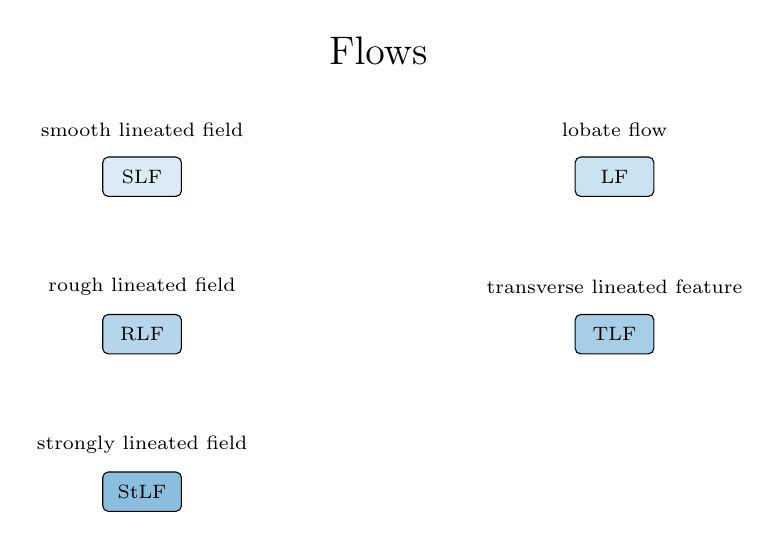
\begin{tikzpicture}[x=3.0cm,y=1.0cm]

\tikzset{
legendunit/.style={
draw=black,
rounded corners=2pt,
minimum width=1.0cm,
minimum height=0.5cm,
font=\scriptsize
},
legendlabel/.style={
align=center,
font=\scriptsize
}
}

%--------------------------------------------------
% HEADER
%--------------------------------------------------

\node[font=\Large] at (1.0,0) {Flows};

%--------------------------------------------------
% LEFT COLUMN
%--------------------------------------------------

\node[legendlabel] at (0,-1) {smooth lineated field};
\node[legendunit,fill=flowblue!25] at (0,-1.6) {SLF};

\node[legendlabel] at (0,-3) {rough lineated field};
\node[legendunit,fill=flowblue!50] at (0,-3.6) {RLF};

\node[legendlabel] at (0,-5) {strongly lineated field};
\node[legendunit,fill=flowblue!80] at (0,-5.6) {StLF};

%--------------------------------------------------
% RIGHT COLUMN
%--------------------------------------------------

\node[legendlabel] at (2,-1) {lobate flow};
\node[legendunit,fill=flowblue!35] at (2,-1.6) {LF};

\node[legendlabel] at (2,-3) {transverse lineated feature};
\node[legendunit,fill=flowblue!60] at (2,-3.6) {TLF};

\end{tikzpicture}

\end{frame}

\begin{frame}{Regional Map Legend}

\centering

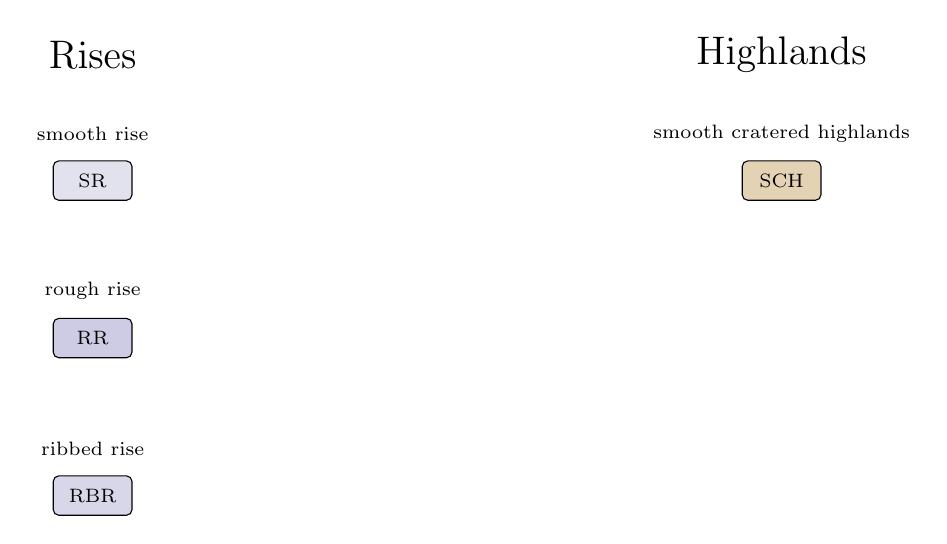
\begin{tikzpicture}[x=3.5cm,y=1.0cm]

\tikzset{
legendunit/.style={
draw=black,
rounded corners=2pt,
minimum width=1.0cm,
minimum height=0.5cm,
font=\scriptsize
},
legendlabel/.style={
align=center,
font=\scriptsize
}
}

%--------------------------------------------------
% HEADERS
%--------------------------------------------------

\node[font=\Large] at (0,0) {Rises};

\node[font=\Large] at (2.5,0) {Highlands};

%--------------------------------------------------
% RISES
%--------------------------------------------------

\node[legendlabel] at (0,-1) {smooth rise};
\node[legendunit,fill=risepurple!30] at (0,-1.6) {SR};

\node[legendlabel] at (0,-3) {rough rise};
\node[legendunit,fill=risepurple!50] at (0,-3.6) {RR};

\node[legendlabel] at (0,-5) {ribbed rise};
\node[legendunit,fill=risepurple!40] at (0,-5.6) {RBR};

%--------------------------------------------------
% HIGHLANDS
%--------------------------------------------------

\node[legendlabel] at (2.5,-1)
{smooth cratered highlands};

\node[legendunit,fill=highlandbrown!50]
at (2.5,-1.6)
{SCH};

\end{tikzpicture}

\end{frame}

\begin{frame}[label=CTXFigMap]{Regional Map}

\begin{figure}
\centering

\begin{subfigure}{0.48\textwidth}
    \centering
    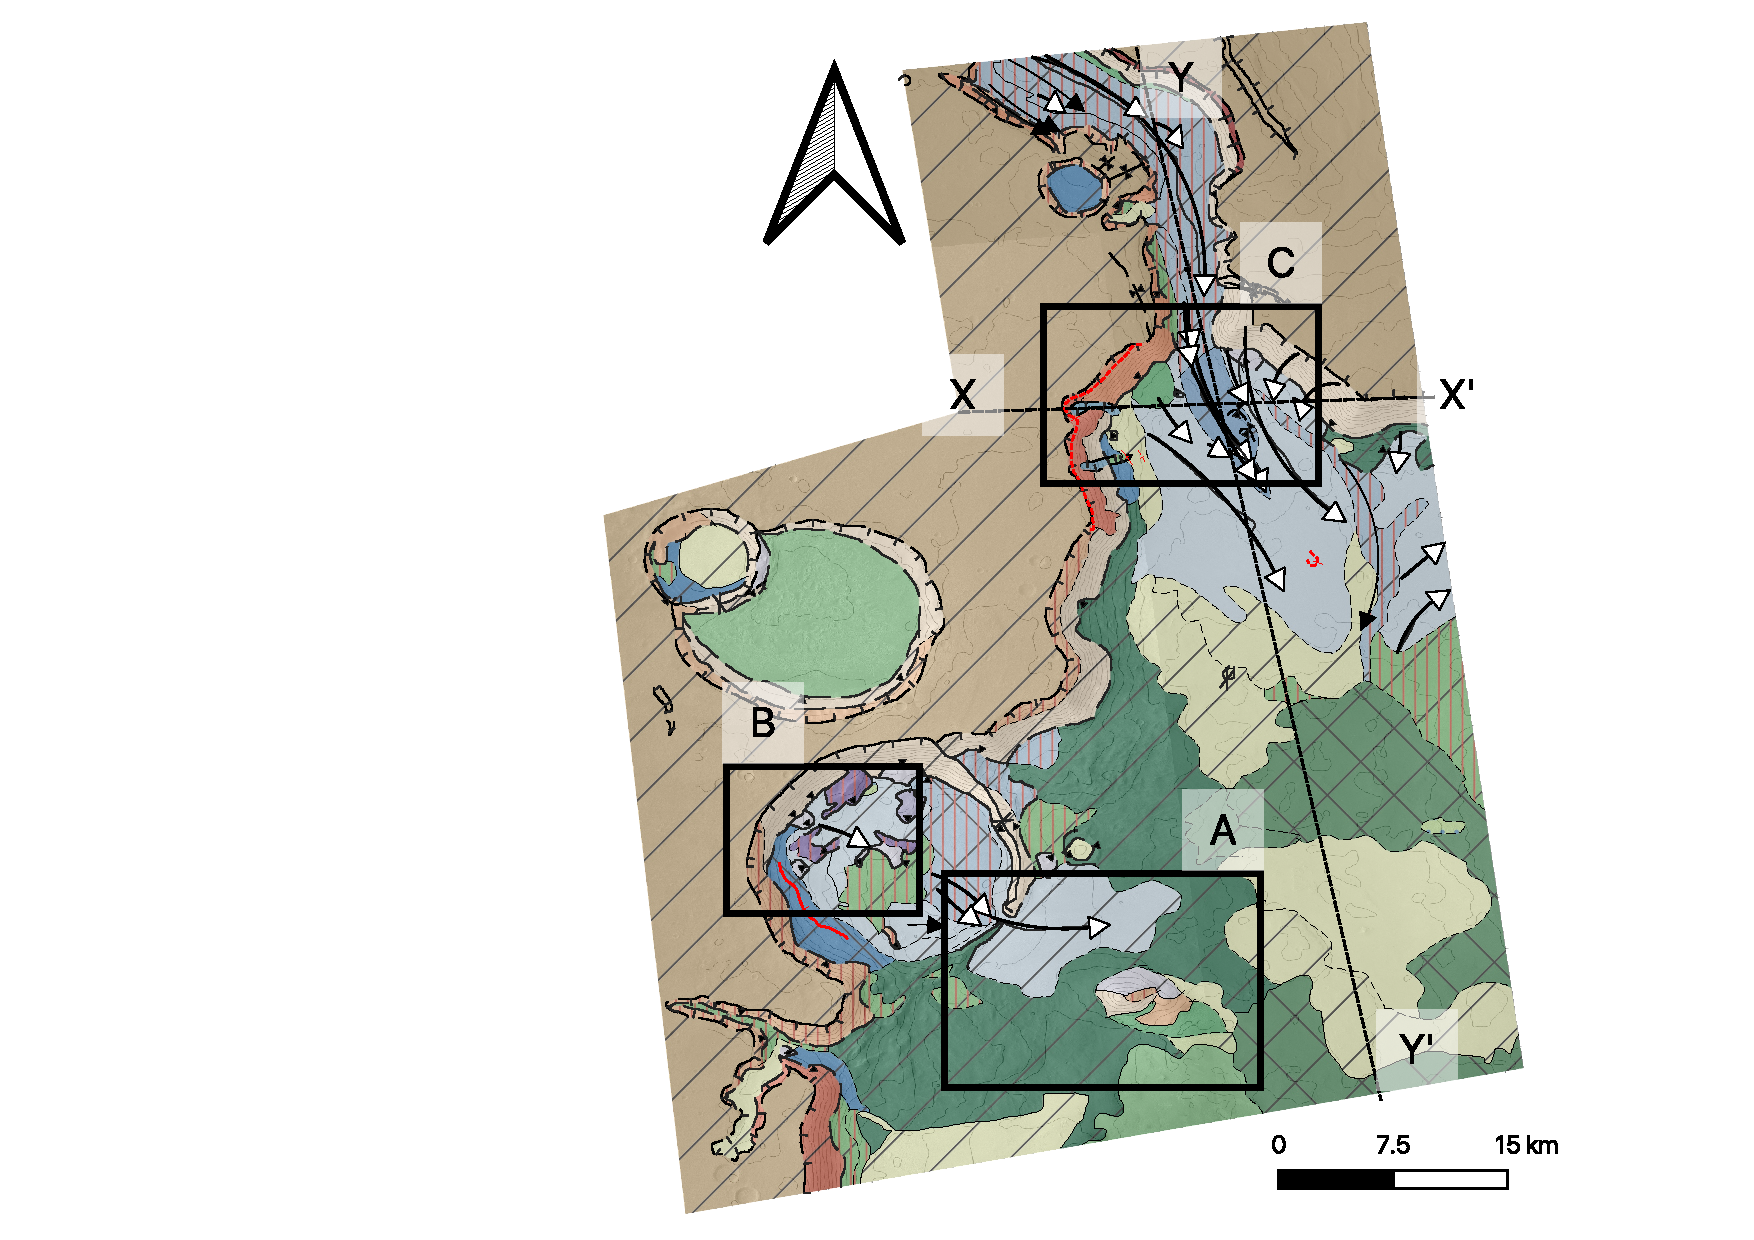
\includegraphics[
        width=\linewidth,
        height=0.65\textheight,
        keepaspectratio
    ]{Figures/Maps/CTX_Final_FigsMap.pdf}
    \label{fig:CTXFinal_a}
\end{subfigure}
\hfill
\begin{subfigure}{0.48\textwidth}
    \centering
    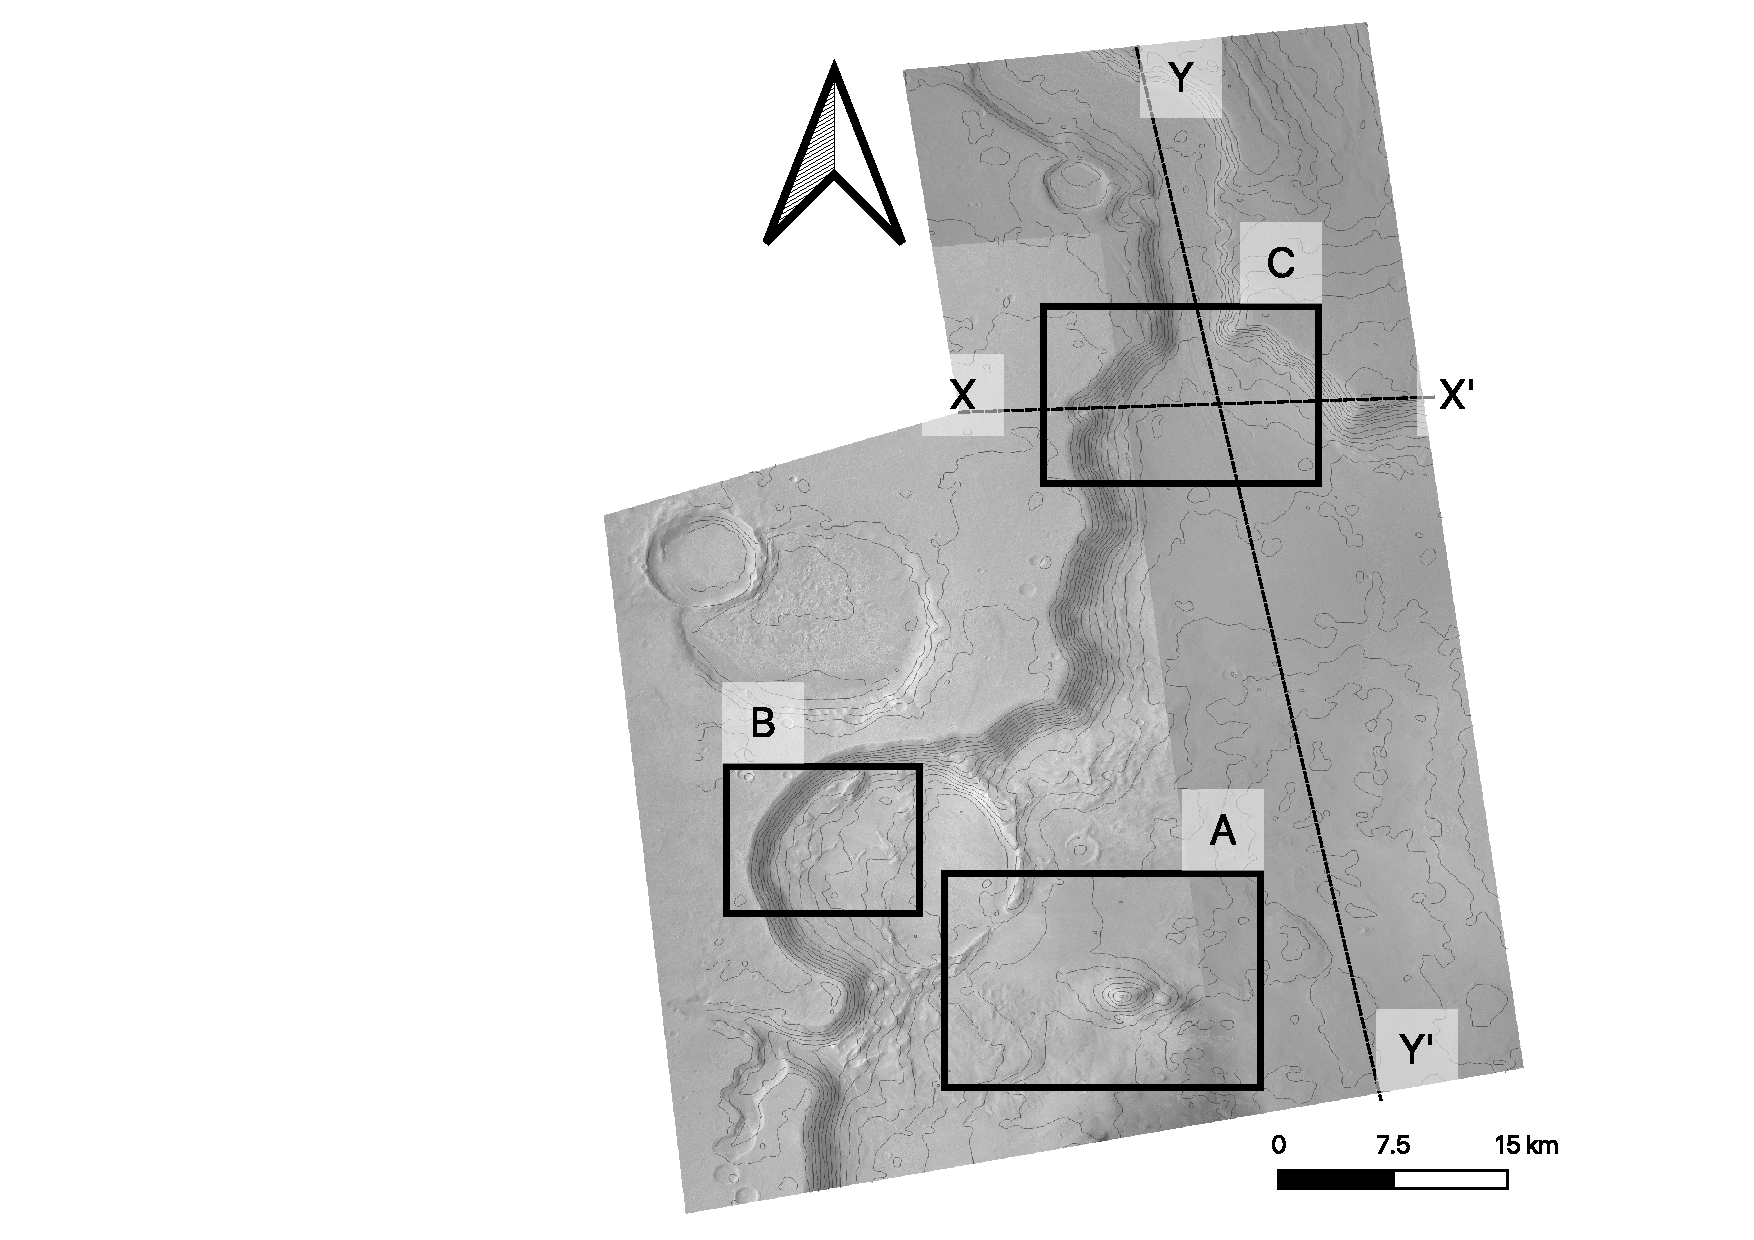
\includegraphics[
        width=\linewidth,
        height=0.65\textheight,
        keepaspectratio
    ]{Figures/Maps/CTX_Final_FigsImg.pdf}
    \label{fig:CTXFinal_b}
\end{subfigure}

\caption{Regional map (from Figure \ref{fig:CTXOverview}) with inserts (A-C; to be shown in alphabetical order) and cross-sections (XX', YY') annotated.}
\label{fig:CTXFinal}
\end{figure}
\end{frame}

\begin{frame}{Subaqueous Retreat and Glacial Modification}

\begin{figure}
\centering

\begin{subfigure}{0.48\textwidth}
    \centering
    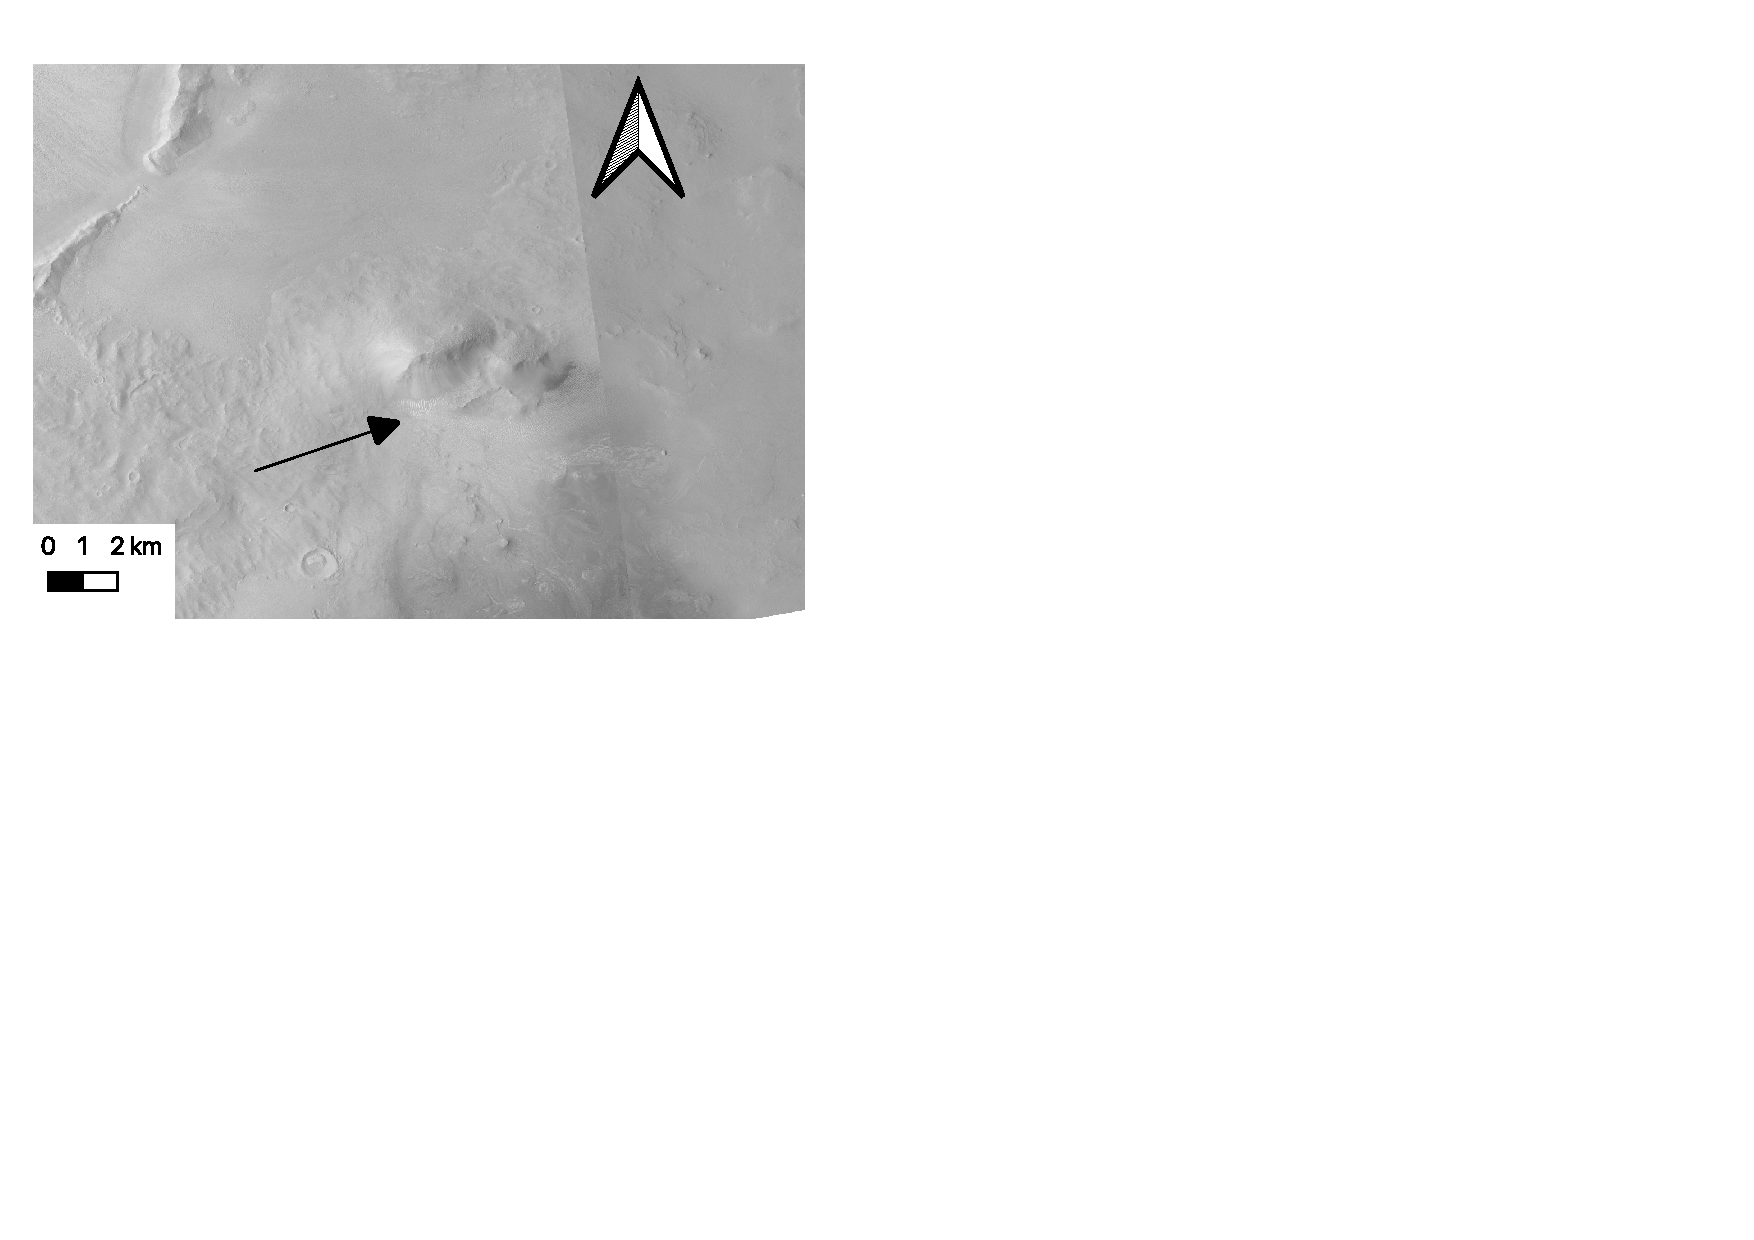
\includegraphics[
        width=\linewidth,
        height=0.65\textheight,
        keepaspectratio
    ]{Figures/CTX/LDM_Img.pdf}
    \label{fig:LDM_a}
\end{subfigure}
\hfill
\begin{subfigure}{0.48\textwidth}
    \centering
    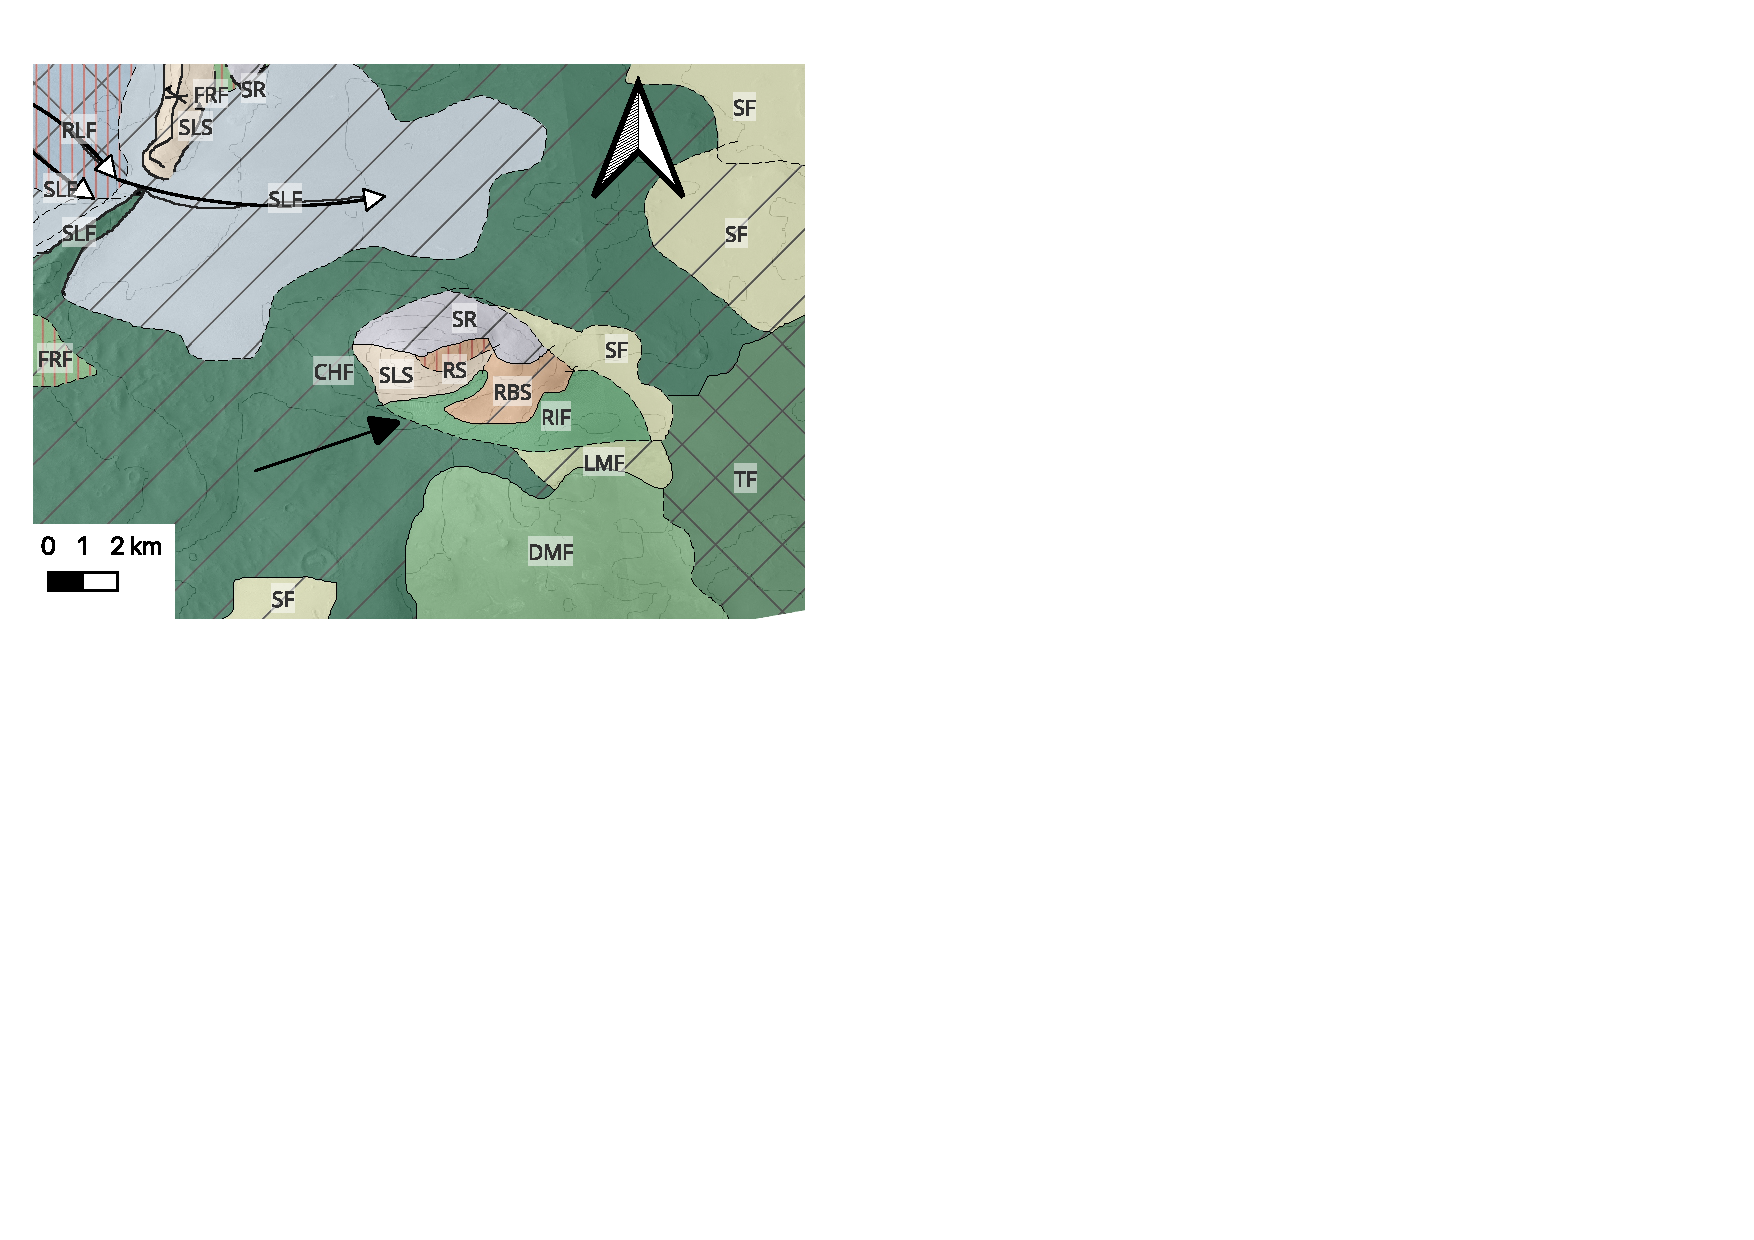
\includegraphics[
        width=\linewidth,
        height=0.65\textheight,
        keepaspectratio
    ]{Figures/CTX/LDM_Map.pdf}
    \label{fig:LDM_b}
\end{subfigure}

\caption{Boundary between lacustrine and glacial influence (centred at $33.97674^{\circ}$N, $16.85247^{\circ}$E).}
\label{fig:LDM}

\end{figure}

\end{frame}

\begin{frame}{Effects of Sublimation within a Crater}

\begin{figure}
\centering

\begin{subfigure}{0.48\textwidth}
    \centering
    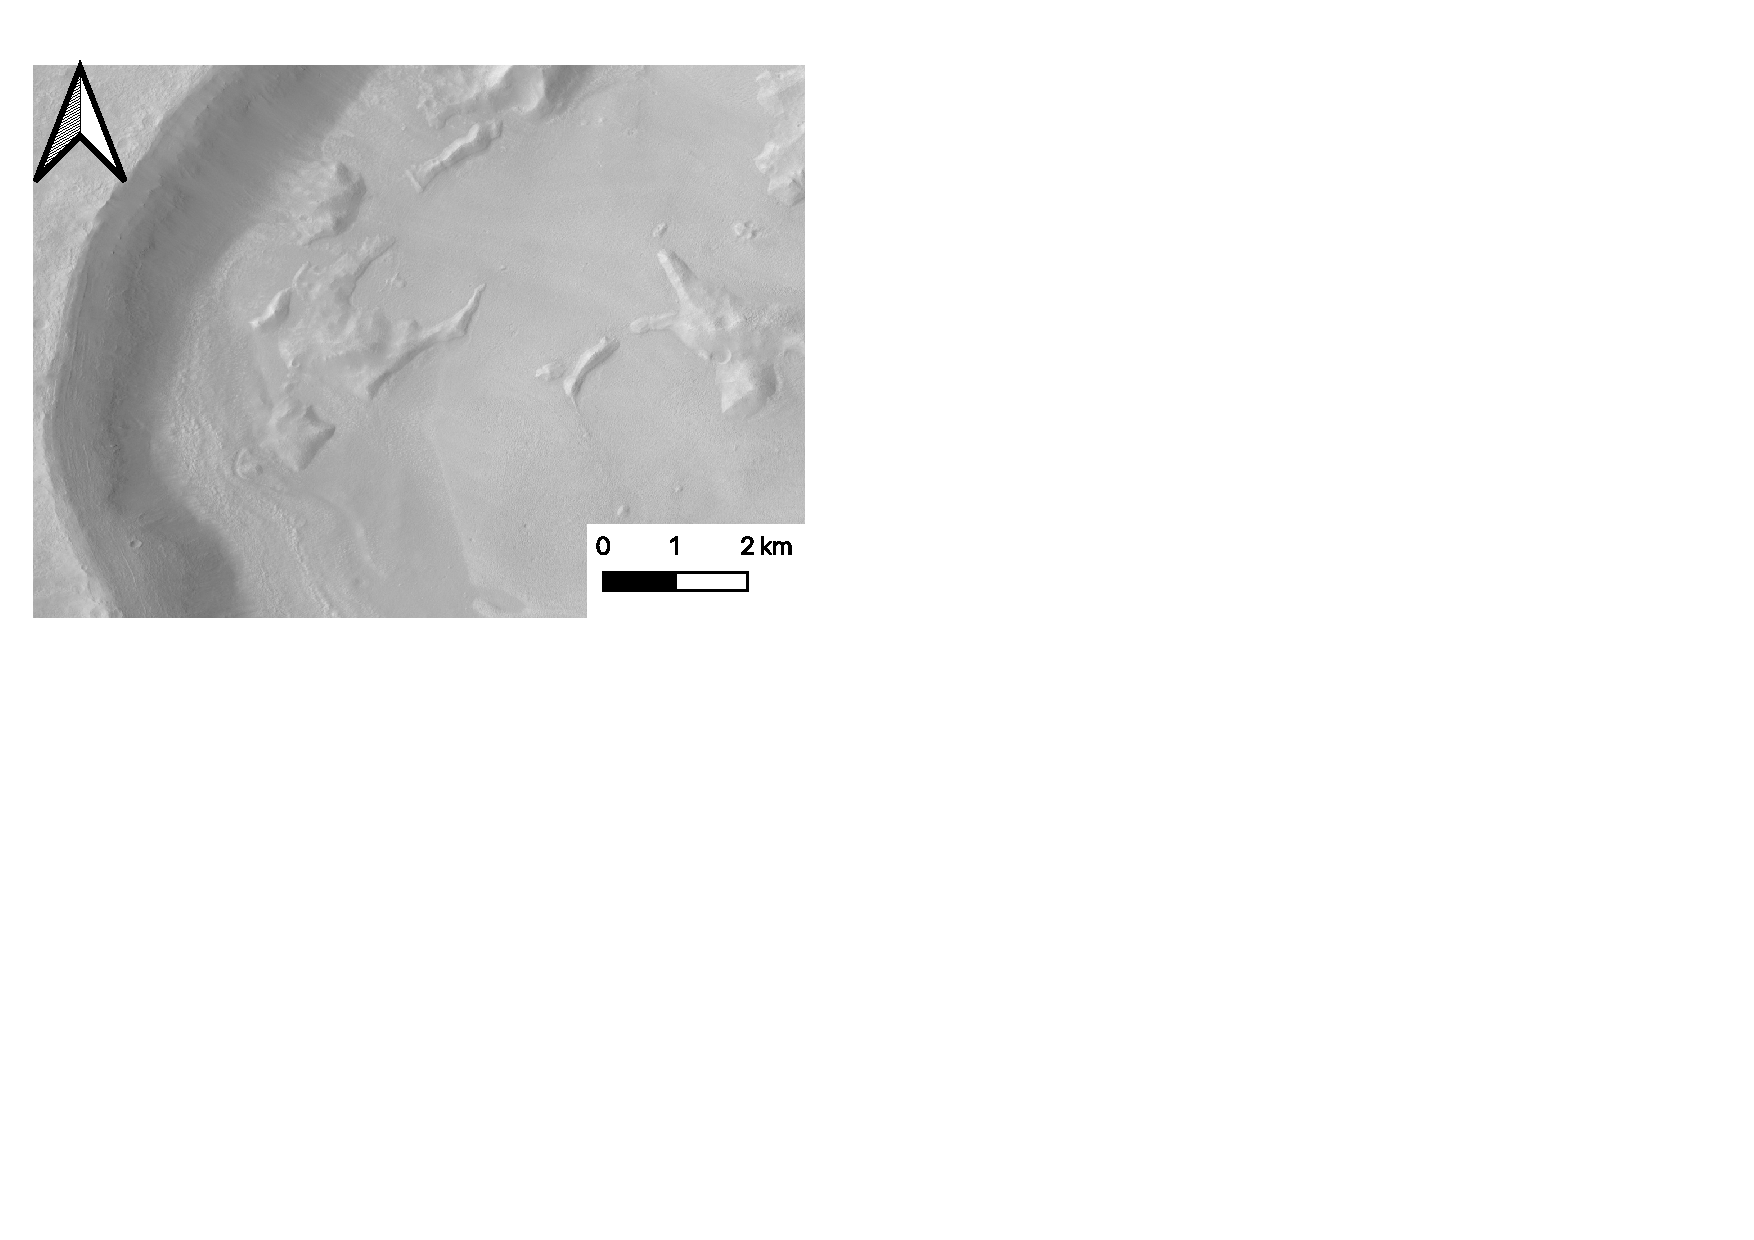
\includegraphics[
        width=\linewidth,
        height=0.65\textheight,
        keepaspectratio
    ]{Figures/CTX/CraterIce_Img.pdf}
    \label{fig:CraterIce_a}
\end{subfigure}
\hfill
\begin{subfigure}{0.48\textwidth}
    \centering
    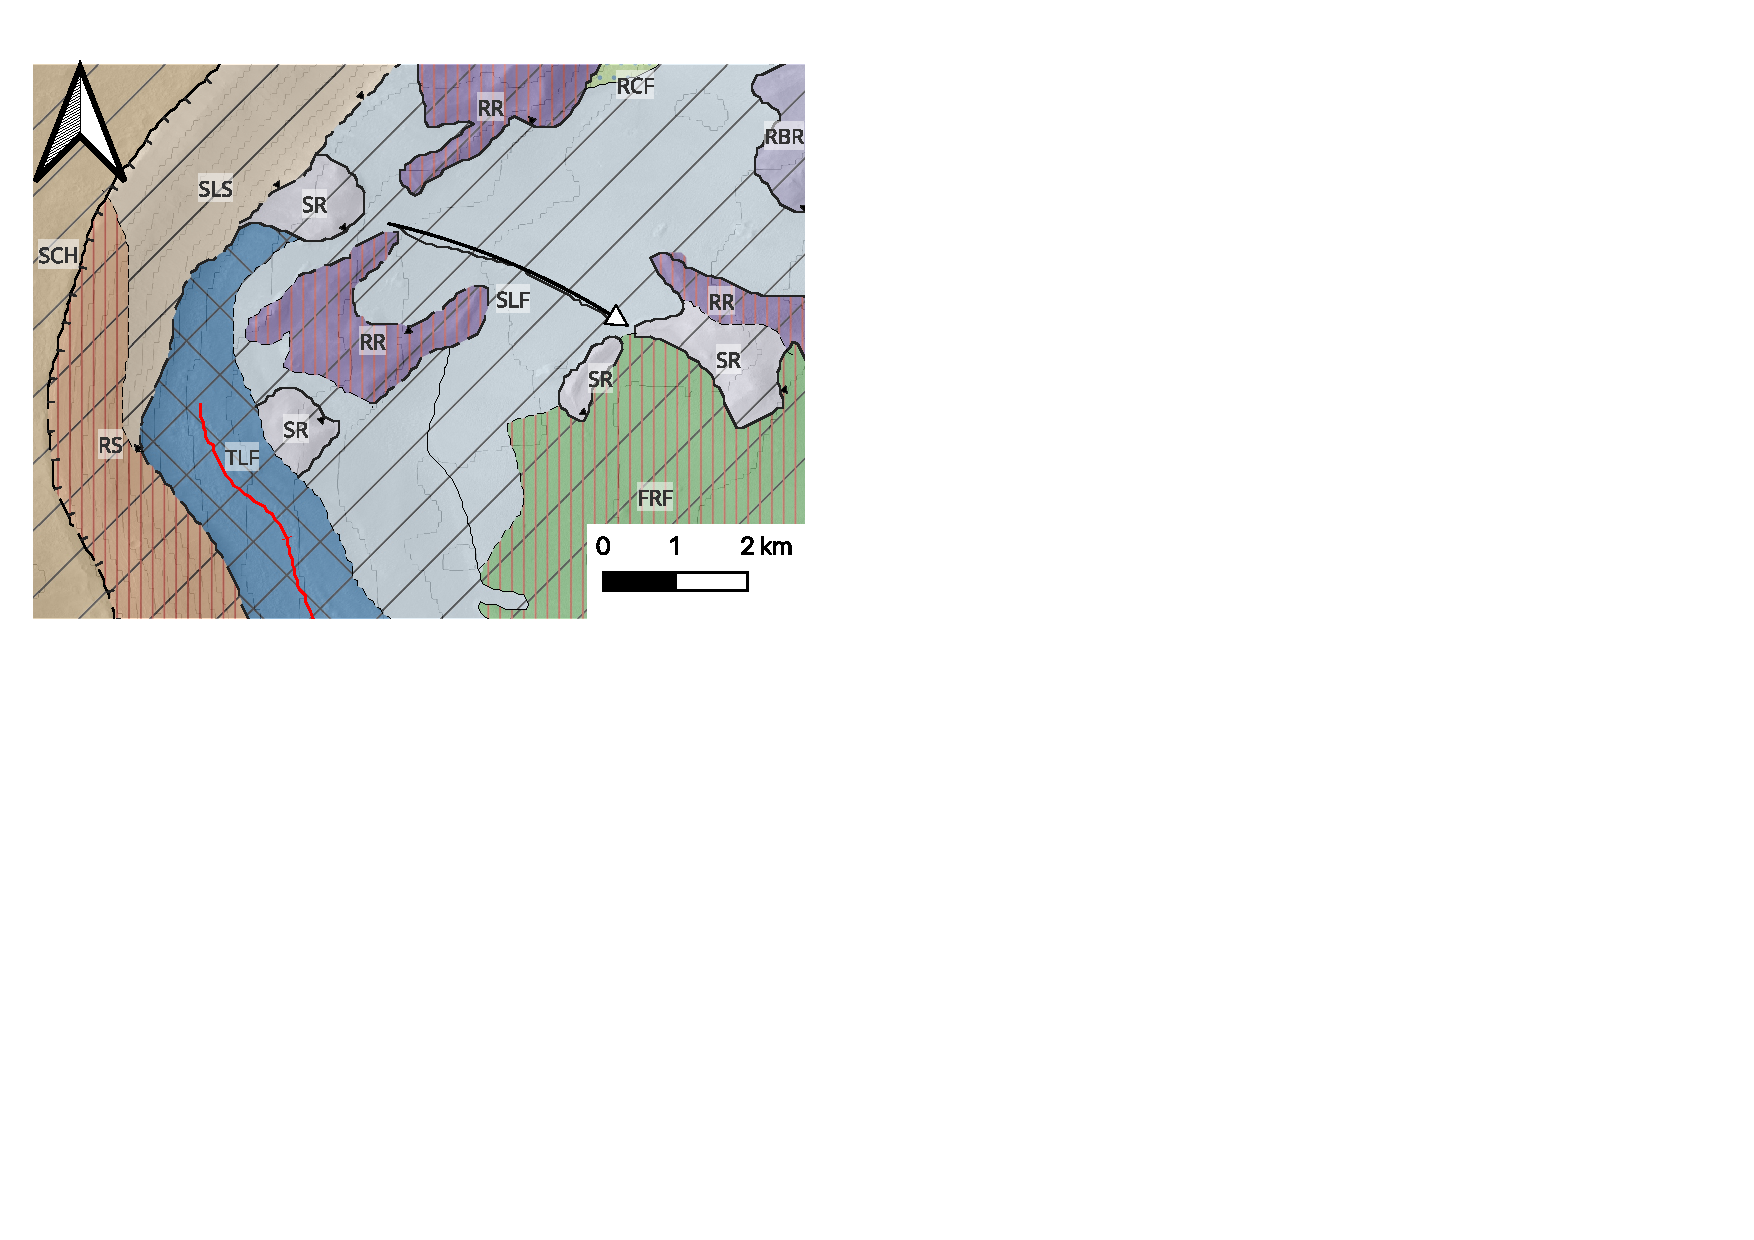
\includegraphics[
        width=\linewidth,
        height=0.65\textheight,
        keepaspectratio
    ]{Figures/CTX/CraterIce_Map.pdf}
    \label{fig:CraterIce_b}
\end{subfigure}

\caption{Crater containing concentric crater fill (CCF) and mesas (centred at $34.14375^{\circ}$N, $16.52417^{\circ}$E).}
\label{fig:CraterIce}

\end{figure}

\end{frame}

\againframe{LargeVFFs}

\begin{frame}{Effects of Sublimation near Mamers Valles}

\begin{figure}
\centering

\begin{subfigure}{0.48\textwidth}
    \centering
    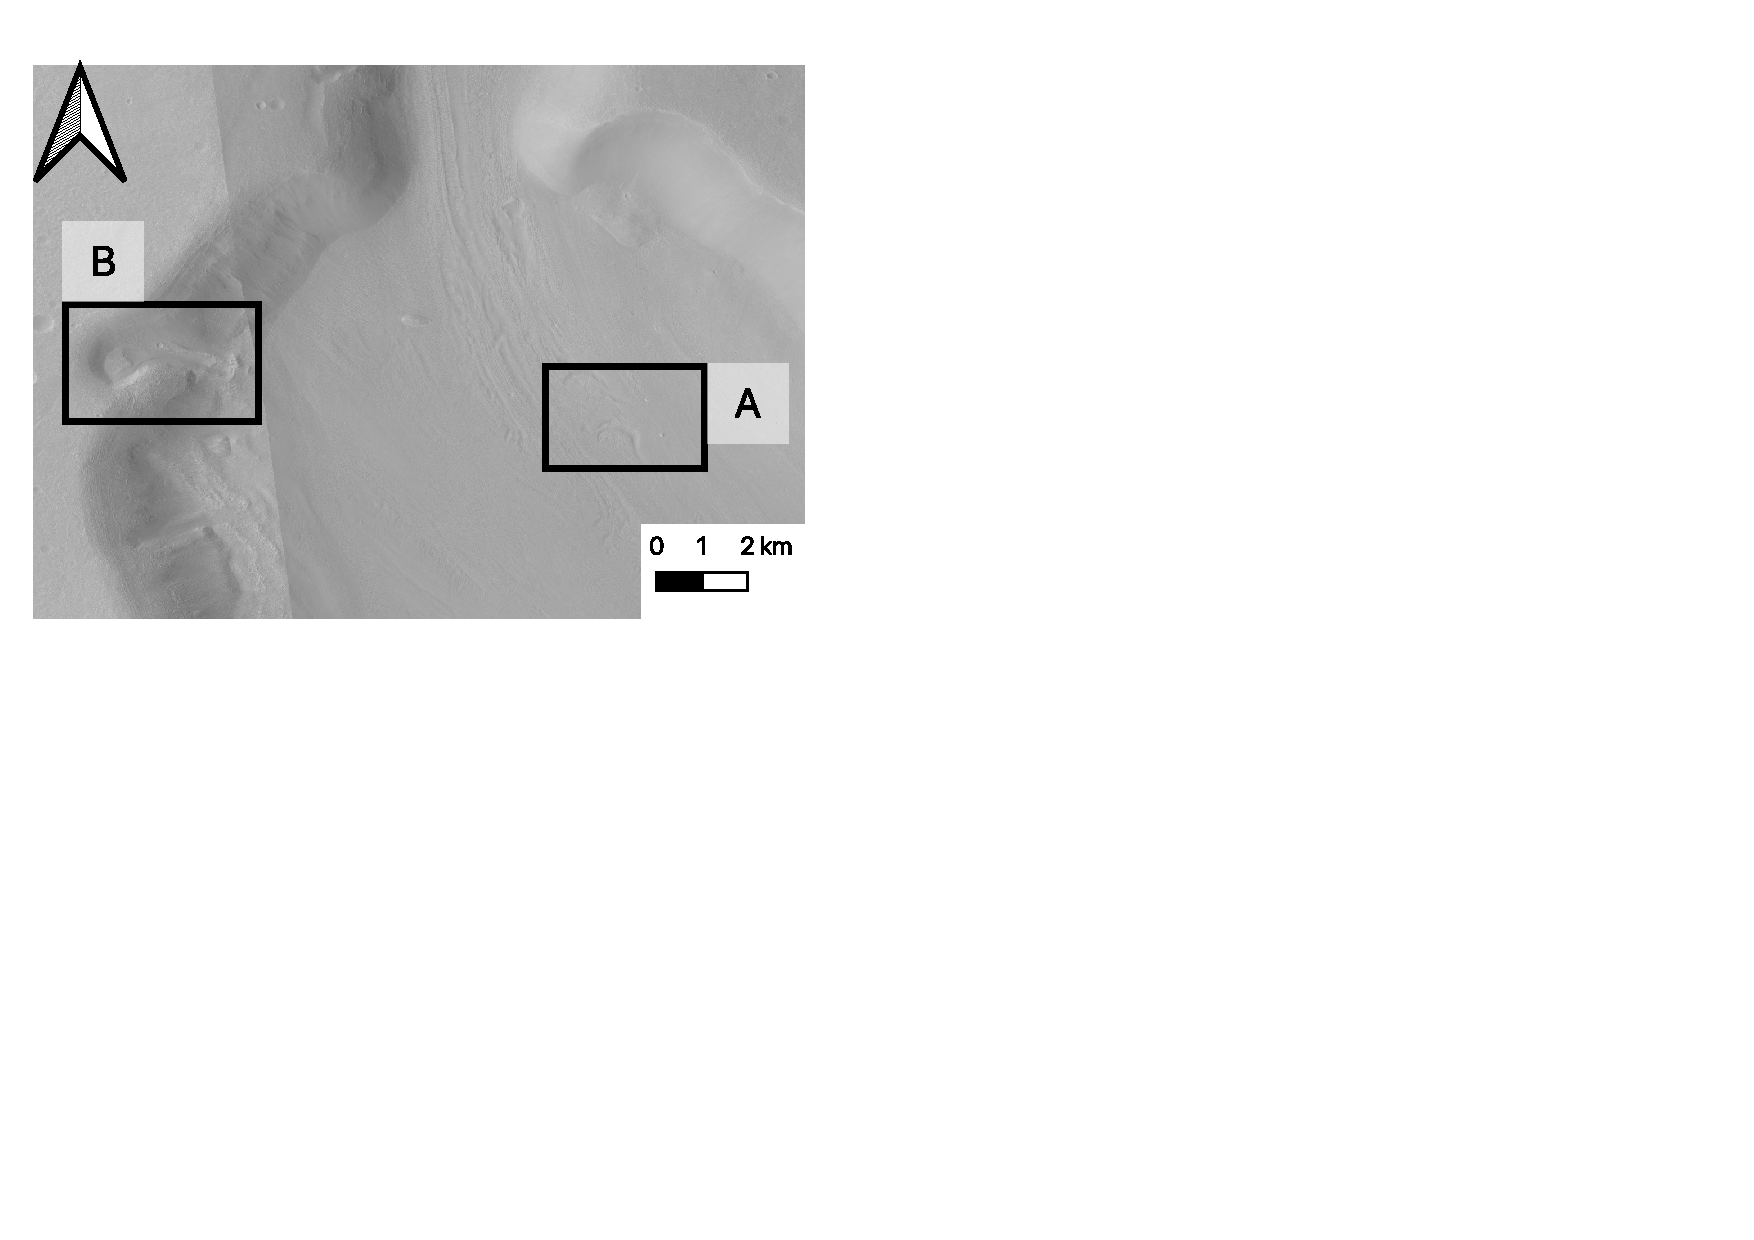
\includegraphics[
        width=\linewidth,
        height=0.65\textheight,
        keepaspectratio
    ]{Figures/CTX/IceActivity_Img.pdf}
    \label{fig:IceActivity_a}
\end{subfigure}
\hfill
\begin{subfigure}{0.48\textwidth}
    \centering
    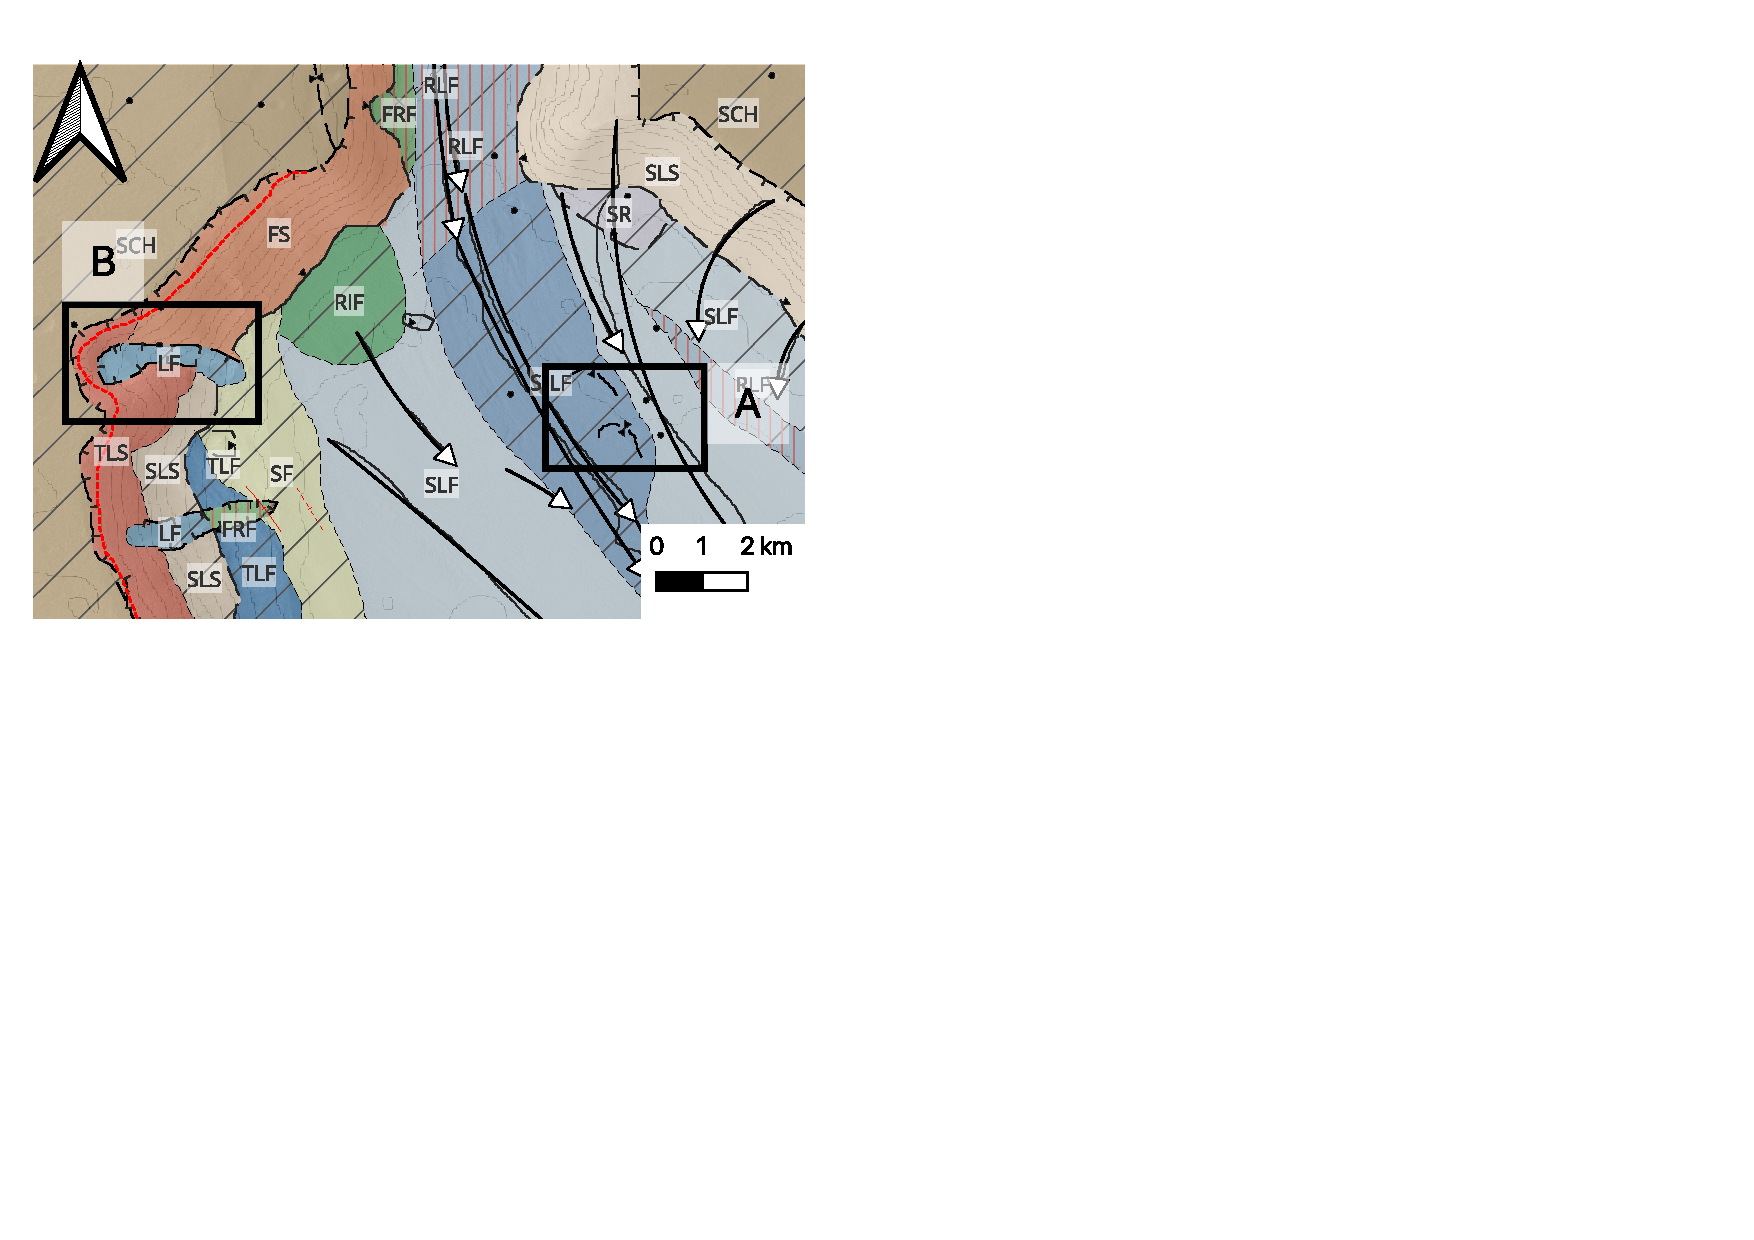
\includegraphics[
        width=\linewidth,
        height=0.65\textheight,
        keepaspectratio
    ]{Figures/CTX/IceActivity_Map.pdf}
    \label{fig:IceActivity_b}
\end{subfigure}

\caption{An overview at the boundary of Ismenius Cavus and the LVF of Mamers Valles (centred at $34.61421^{\circ}$N, $16.92877^{\circ}$E).}
\label{fig:IceActivity}

\end{figure}

\end{frame}

\begin{frame}{Effects of Sublimation near Mamers Valles}
    \begin{figure}
        \centering
        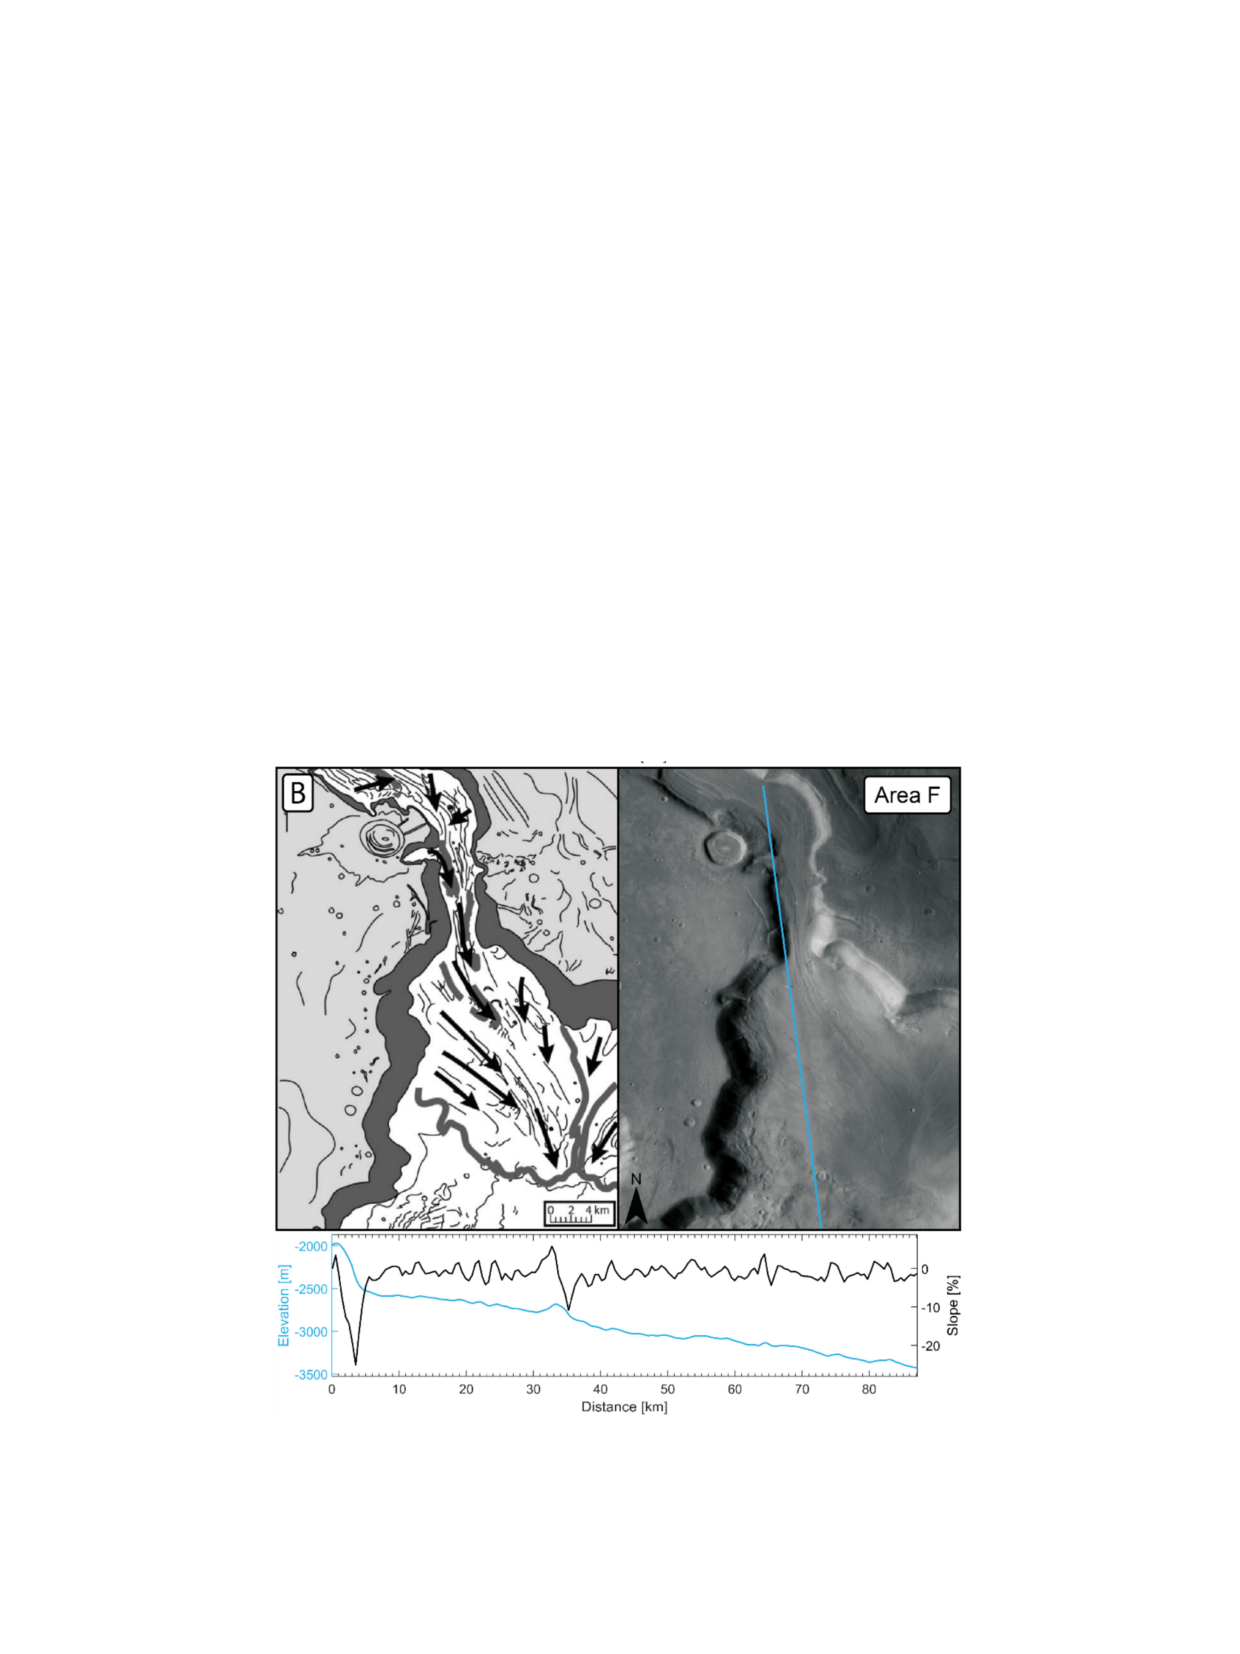
\includegraphics[
        width=\linewidth,
        height=0.65\textheight,
        keepaspectratio]
        {Figures/Diagrams/Wueller25_Fig4}
    \caption{Annotated CTX image data, showing the flow of LVF from Mamers Valles into Ismenius Cavus and the corresponding HRSC-MOLA topographic profile (Figure from \cite{Wueller25}).}
    \end{figure}
\end{frame}

\begin{frame}{Effects of Sublimation near Mamers Valles}

\begin{figure}
\centering
\begin{subfigure}{0.48\textwidth}
    \centering
    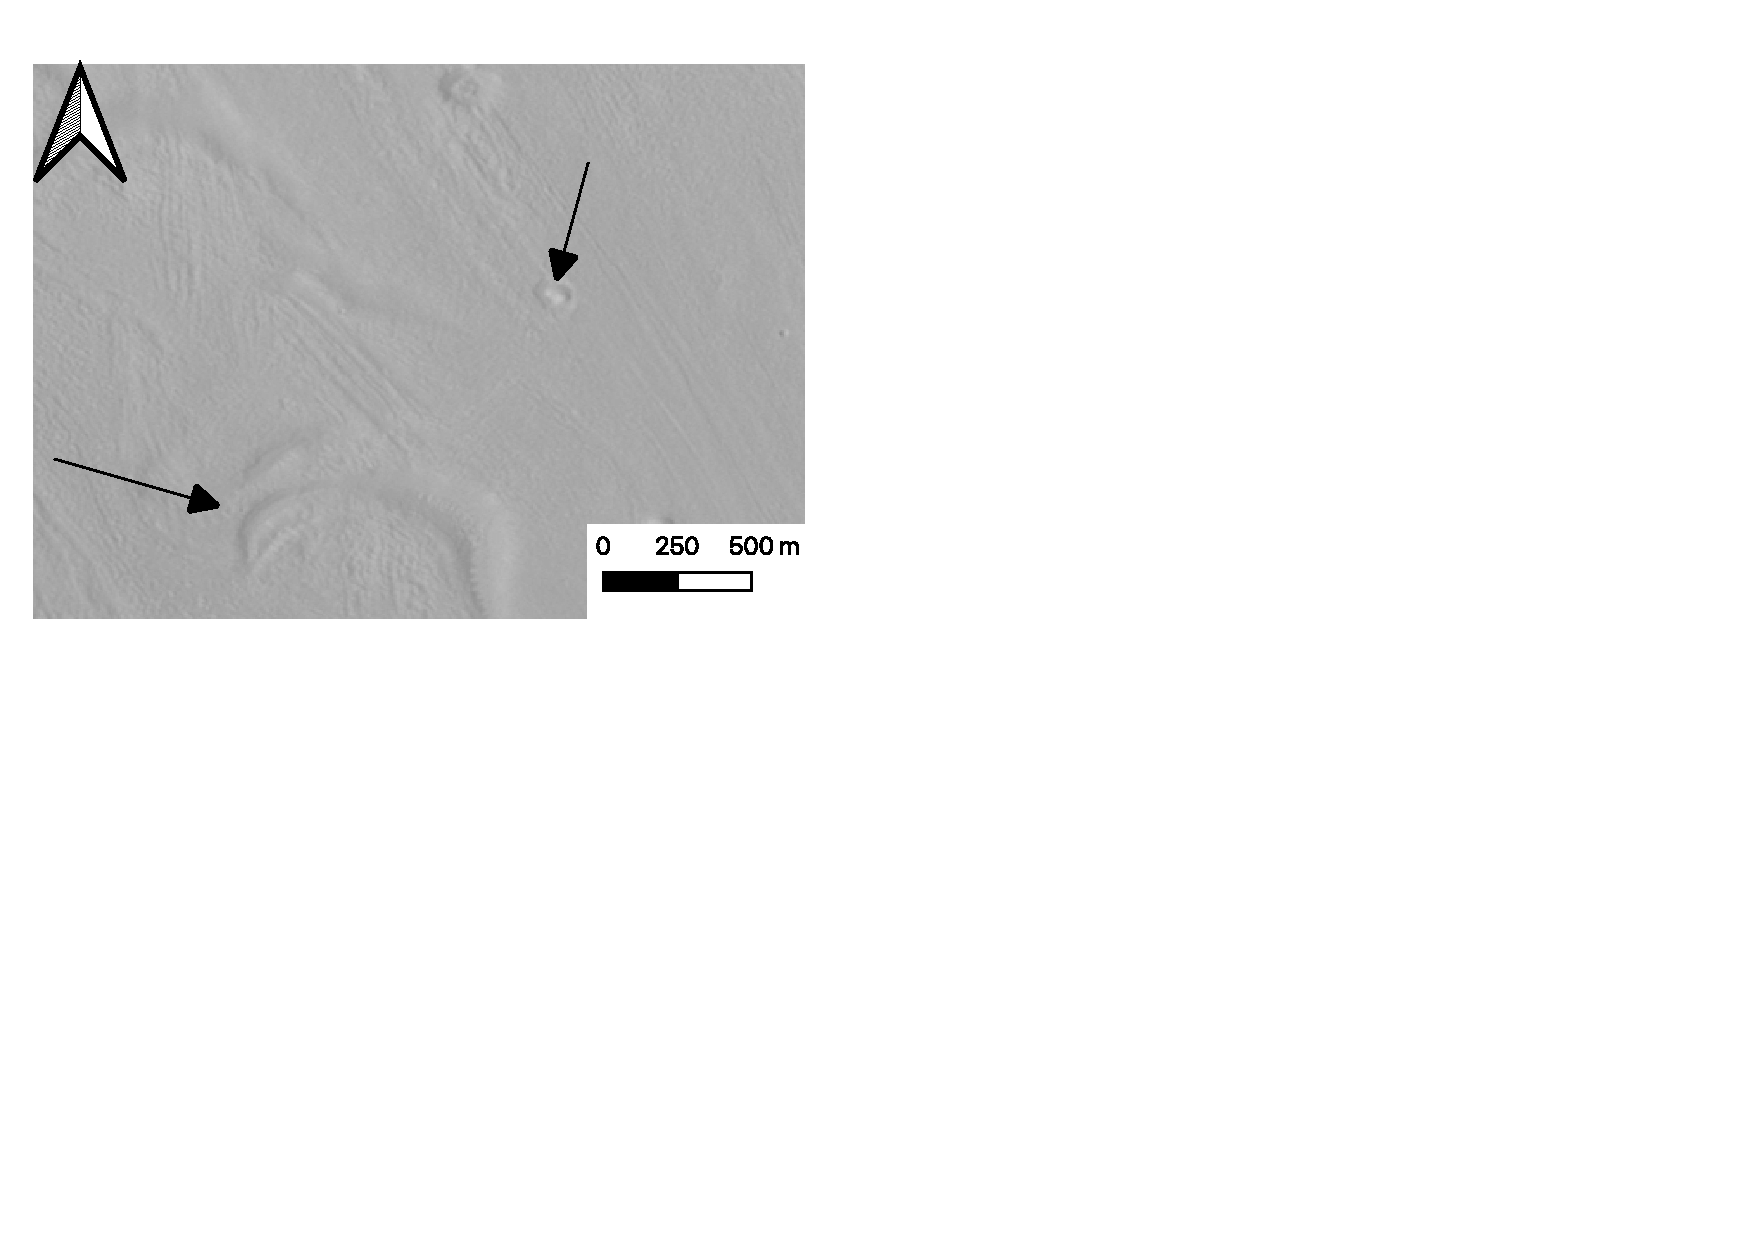
\includegraphics[
        width=\linewidth,
        height=0.65\textheight,
        keepaspectratio
    ]{Figures/CTX/IceActivityZoom_Img.pdf}
    \label{fig:IceActivityZoom_a}
\end{subfigure}
\hfill
\begin{subfigure}{0.48\textwidth}
    \centering
    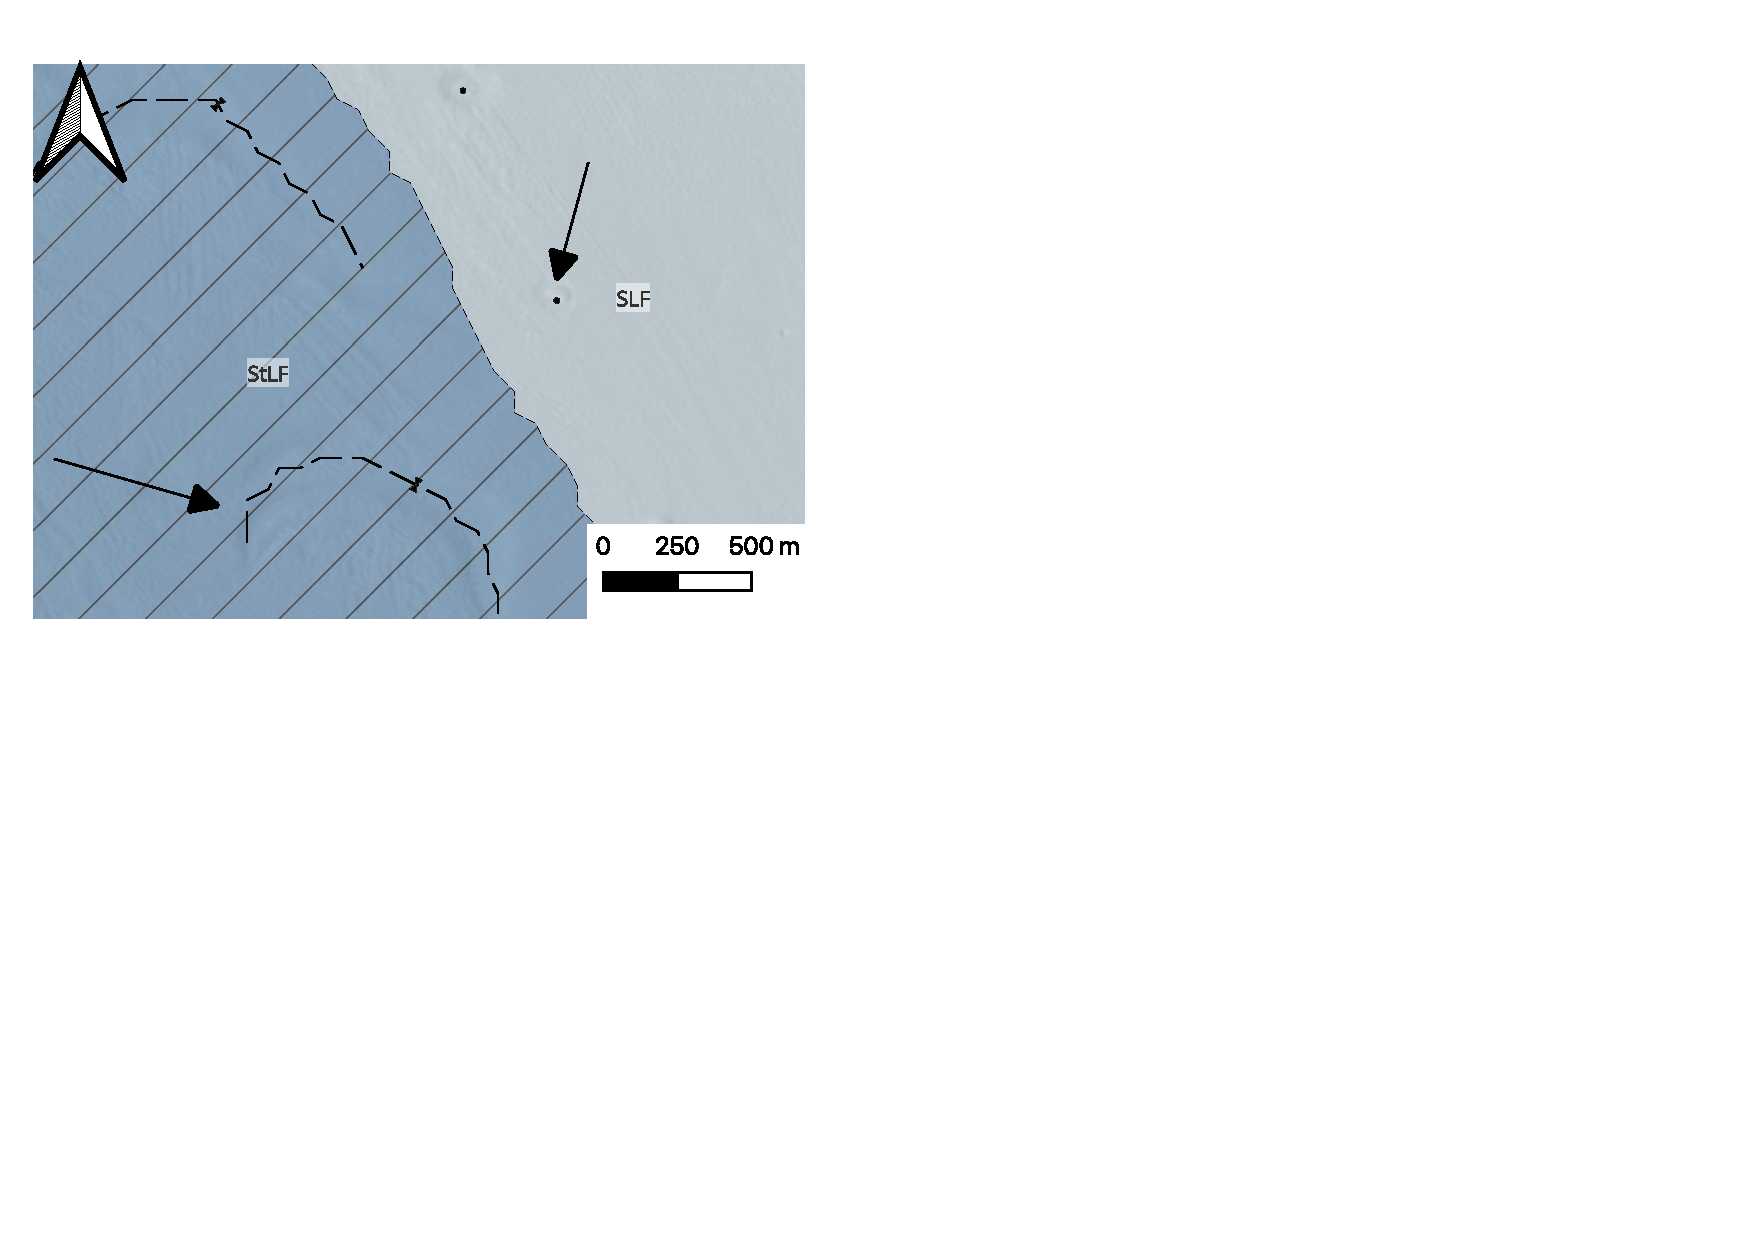
\includegraphics[
        width=\linewidth,
        height=0.65\textheight,
        keepaspectratio
    ]{Figures/CTX/IceActivityZoom_Map.pdf}
    \label{fig:IceActivityZoom_b}
\end{subfigure}

\caption{Sublimation-related erosional features near Mamers Valles. A ring-mold crater (right) and crevasse (left) are highlighted (centred at $34.61601^{\circ}$N, $16.97785^{\circ}$E).}
\label{fig:IceActivityZoom}

\end{figure}

\end{frame}

\againframe{RingMold}


\begin{frame}{Regional Stratigraphic Column}

\begin{figure}
\centering
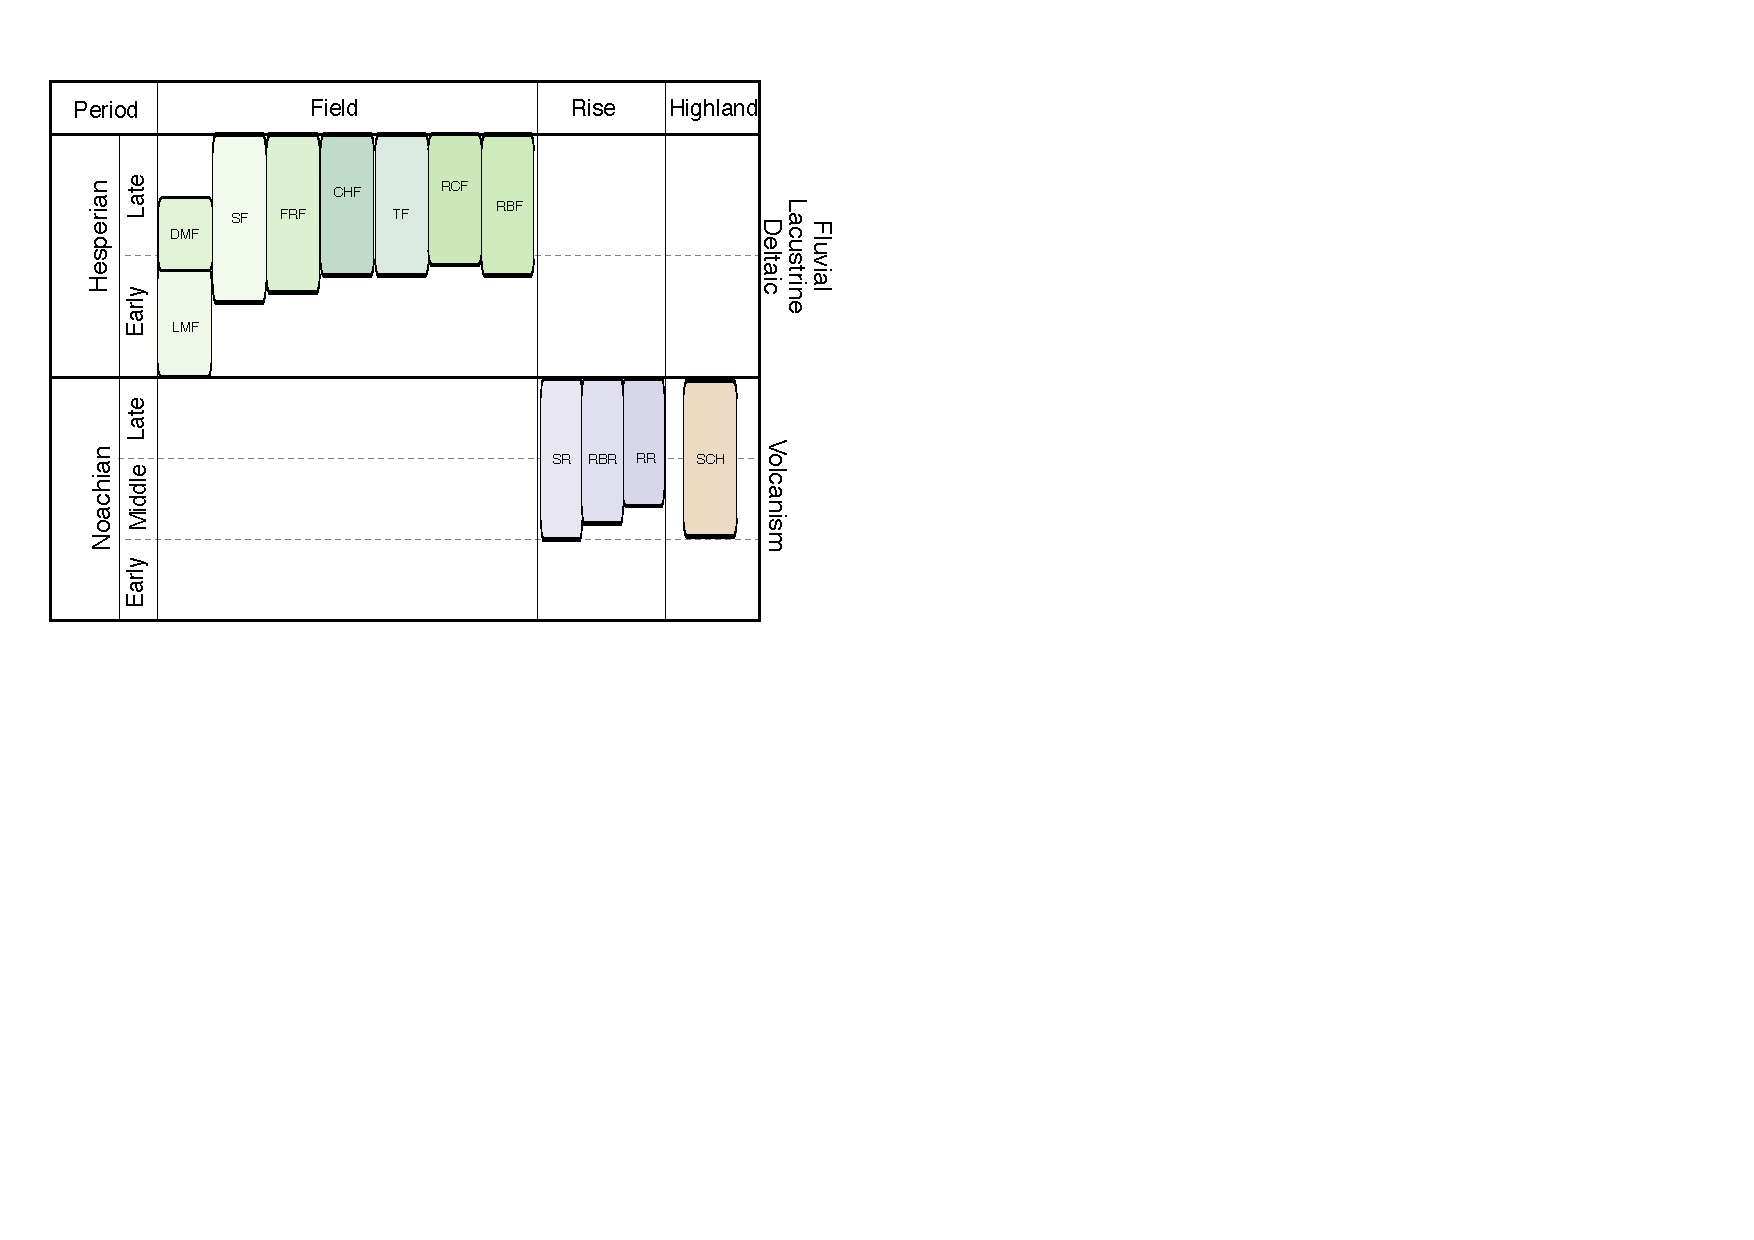
\includegraphics[
    height=0.6\textheight,
    keepaspectratio
]{Figures/Cross_Sec/StratColNH.pdf}
\label{fig:NHCTXCrossSec}
\end{figure}
\sidecite{Informed by \cite{Wueller24,Moro25}.}
\end{frame}

\begin{frame}{Regional Stratigraphic Column}

\begin{figure}
\centering
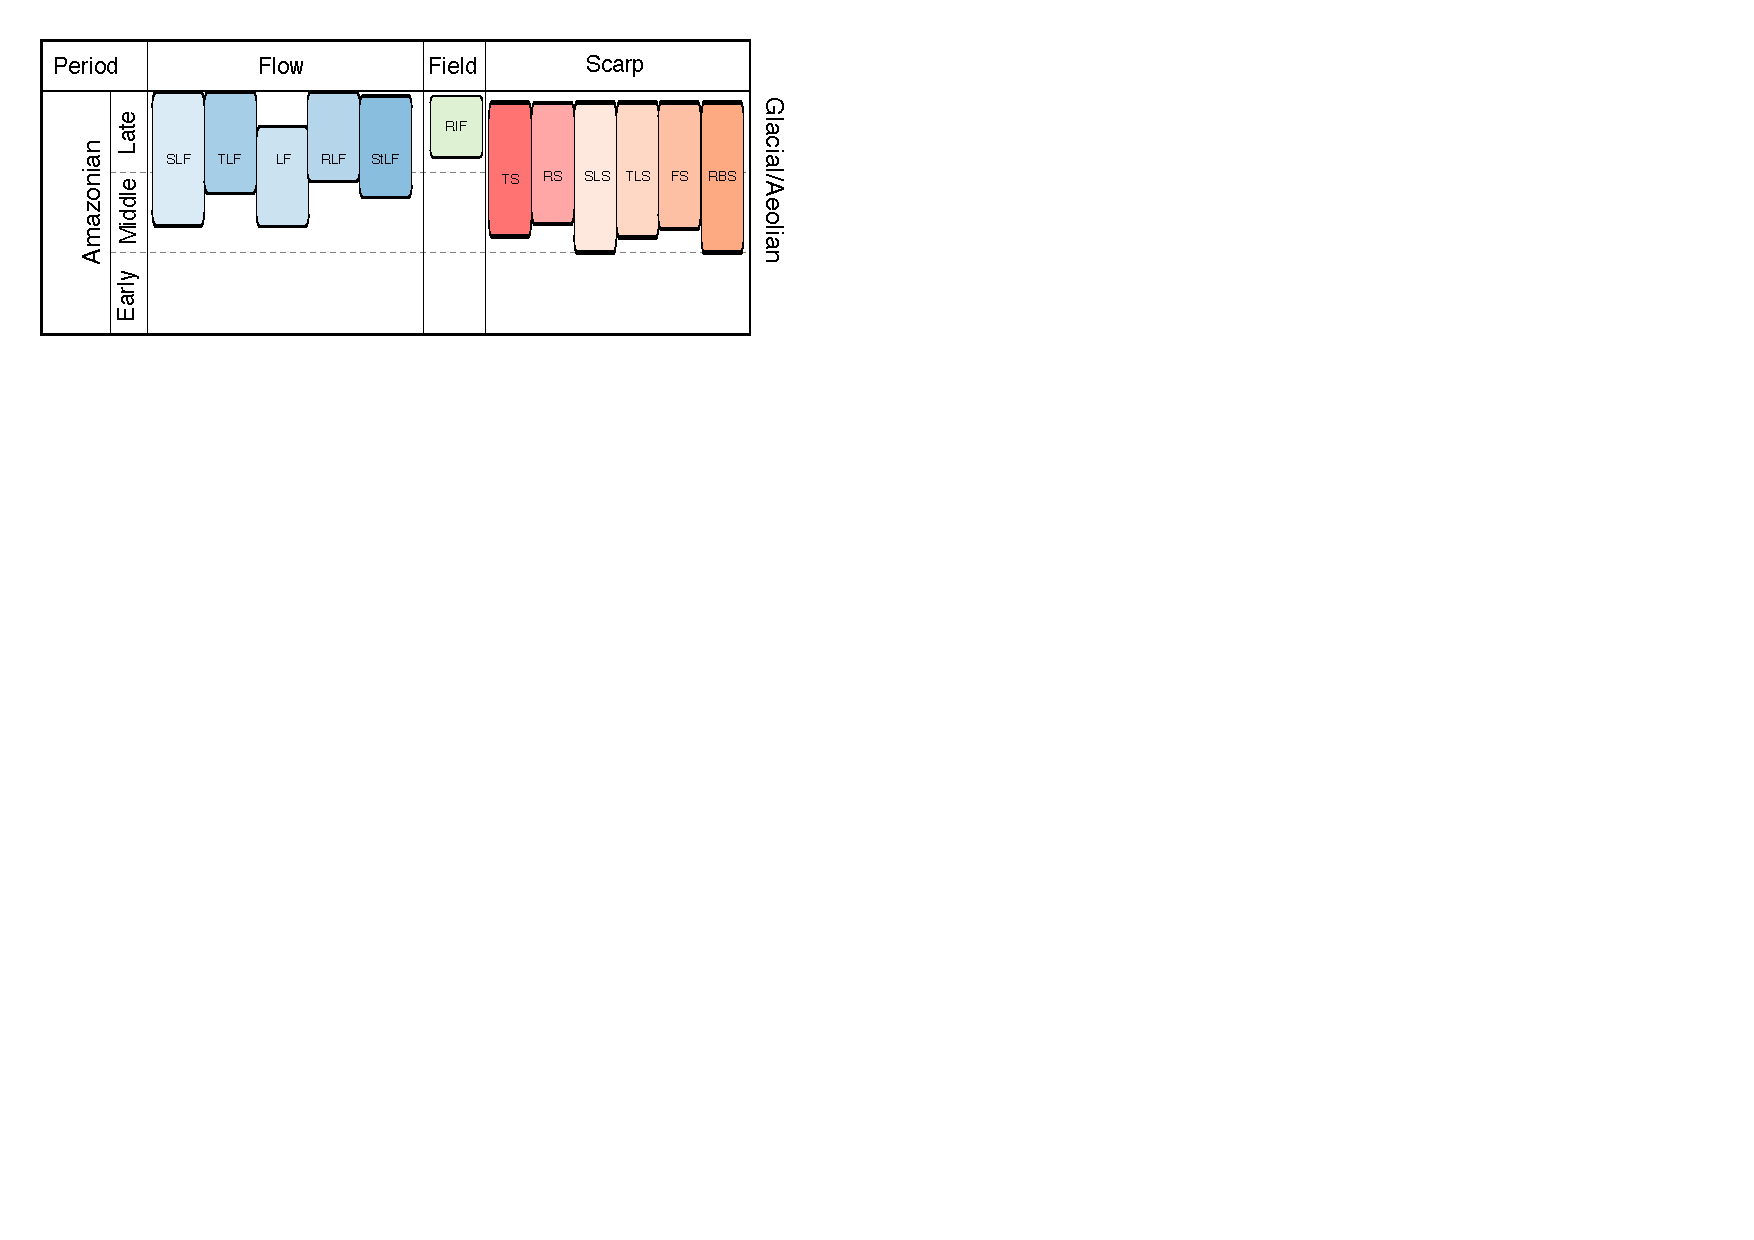
\includegraphics[
    height=0.5\textheight,
    keepaspectratio
]{Figures/Cross_Sec/StratColA.pdf}
\label{fig:ACTXCrossSec}
\end{figure}
\sidecite{Informed by \cite{Wueller24,Moro25}.}
\end{frame}
\againframe{CTXFigMap}
\begin{frame}{Cross-Section Parallel to Flow}
\begin{figure}
    \centering
    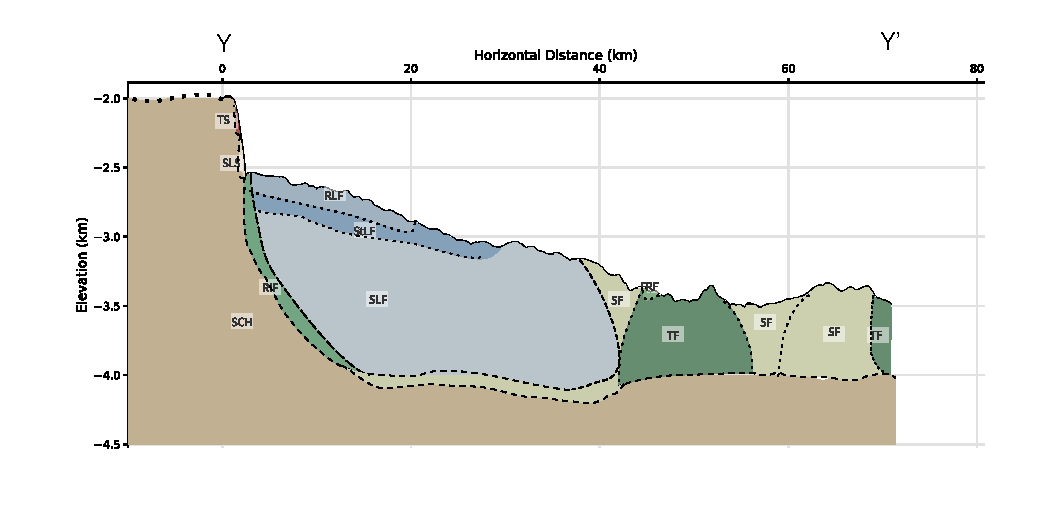
\includegraphics[
        width=\linewidth,
        height=0.65\textheight,
        keepaspectratio
    ]{Figures/Cross_Sec/Cross_Section_NS.pdf}
    \caption{Cross-section made parallel to flow (north-south). Elevation data from the HRSC DEM. }
    \label{fig:CrossSection_NS}
\end{figure}
\sidecite{Informed by \cite{Baker15}.}
\end{frame}
\begin{frame}{Cross-Section Transverse to Flow}

\begin{figure}
    \centering
    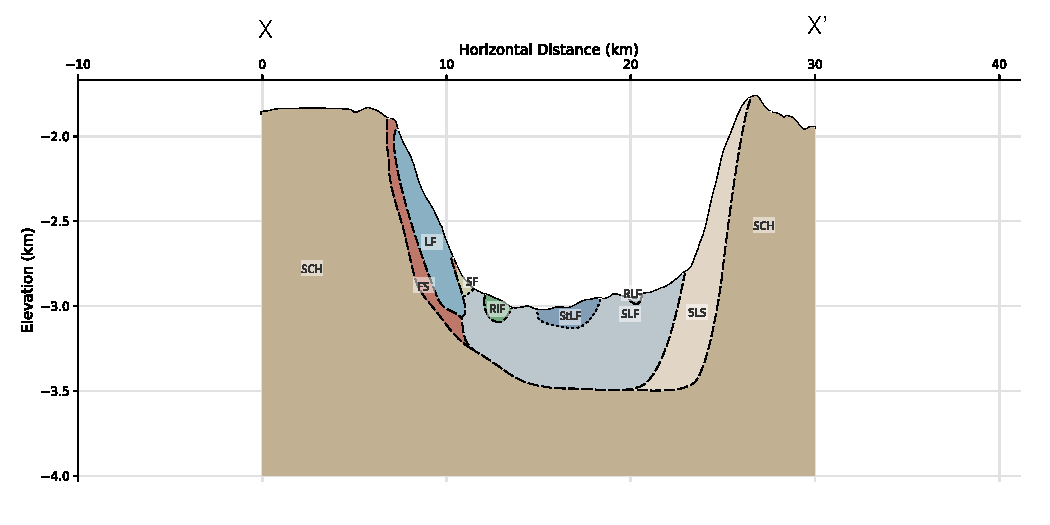
\includegraphics[
        width=\linewidth,
        height=0.65\textheight,
        keepaspectratio
    ]{Figures/Cross_Sec/Cross_Section_EW.pdf}
    \caption{Cross-section made transverse to flow (east-west). Elevation data from the HRSC DEM.}
    \label{fig:CrossSection_EW}
\end{figure}
\sidecite{Informed by \cite{Baker15}.}
\end{frame}

%%%%%%%%%%%%%%%%%%%%%%%%%%%%%%%%%%%%%%
\section{Formation of Alcove Feature}
%%%%%%%%%%%%%%%%%%%%%%%%%%%%%%%%%%%%%%
\againframe{CTXFigMap}

\begin{frame}{Alcove Feature Map}

\begin{figure}
\centering

\begin{subfigure}{0.48\textwidth}
    \centering
    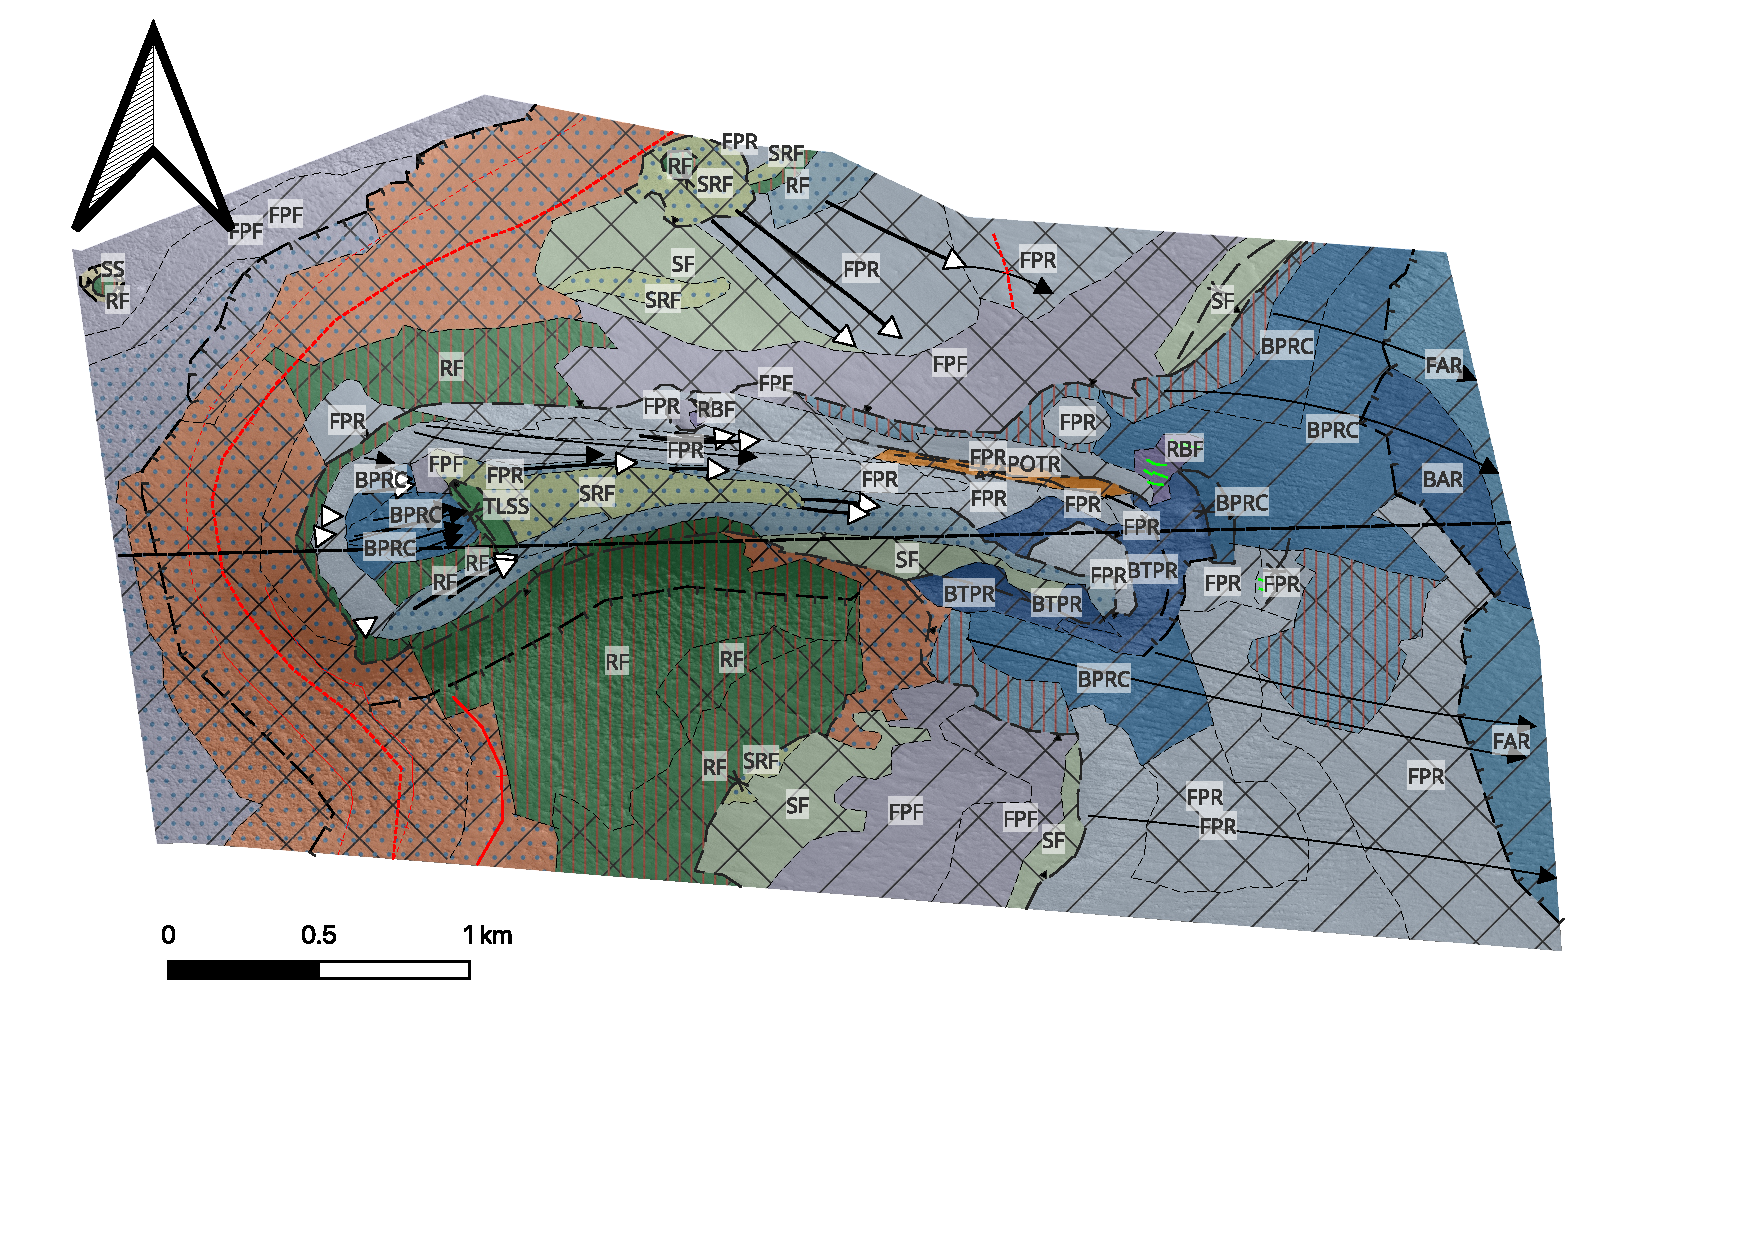
\includegraphics[
        width=\linewidth,
        height=0.65\textheight,
        keepaspectratio
    ]{Figures/Maps/HiRISE_Final_Map.pdf}
    \label{fig:HiRISEOverview_a}
\end{subfigure}
\hfill
\begin{subfigure}{0.48\textwidth}
    \centering
    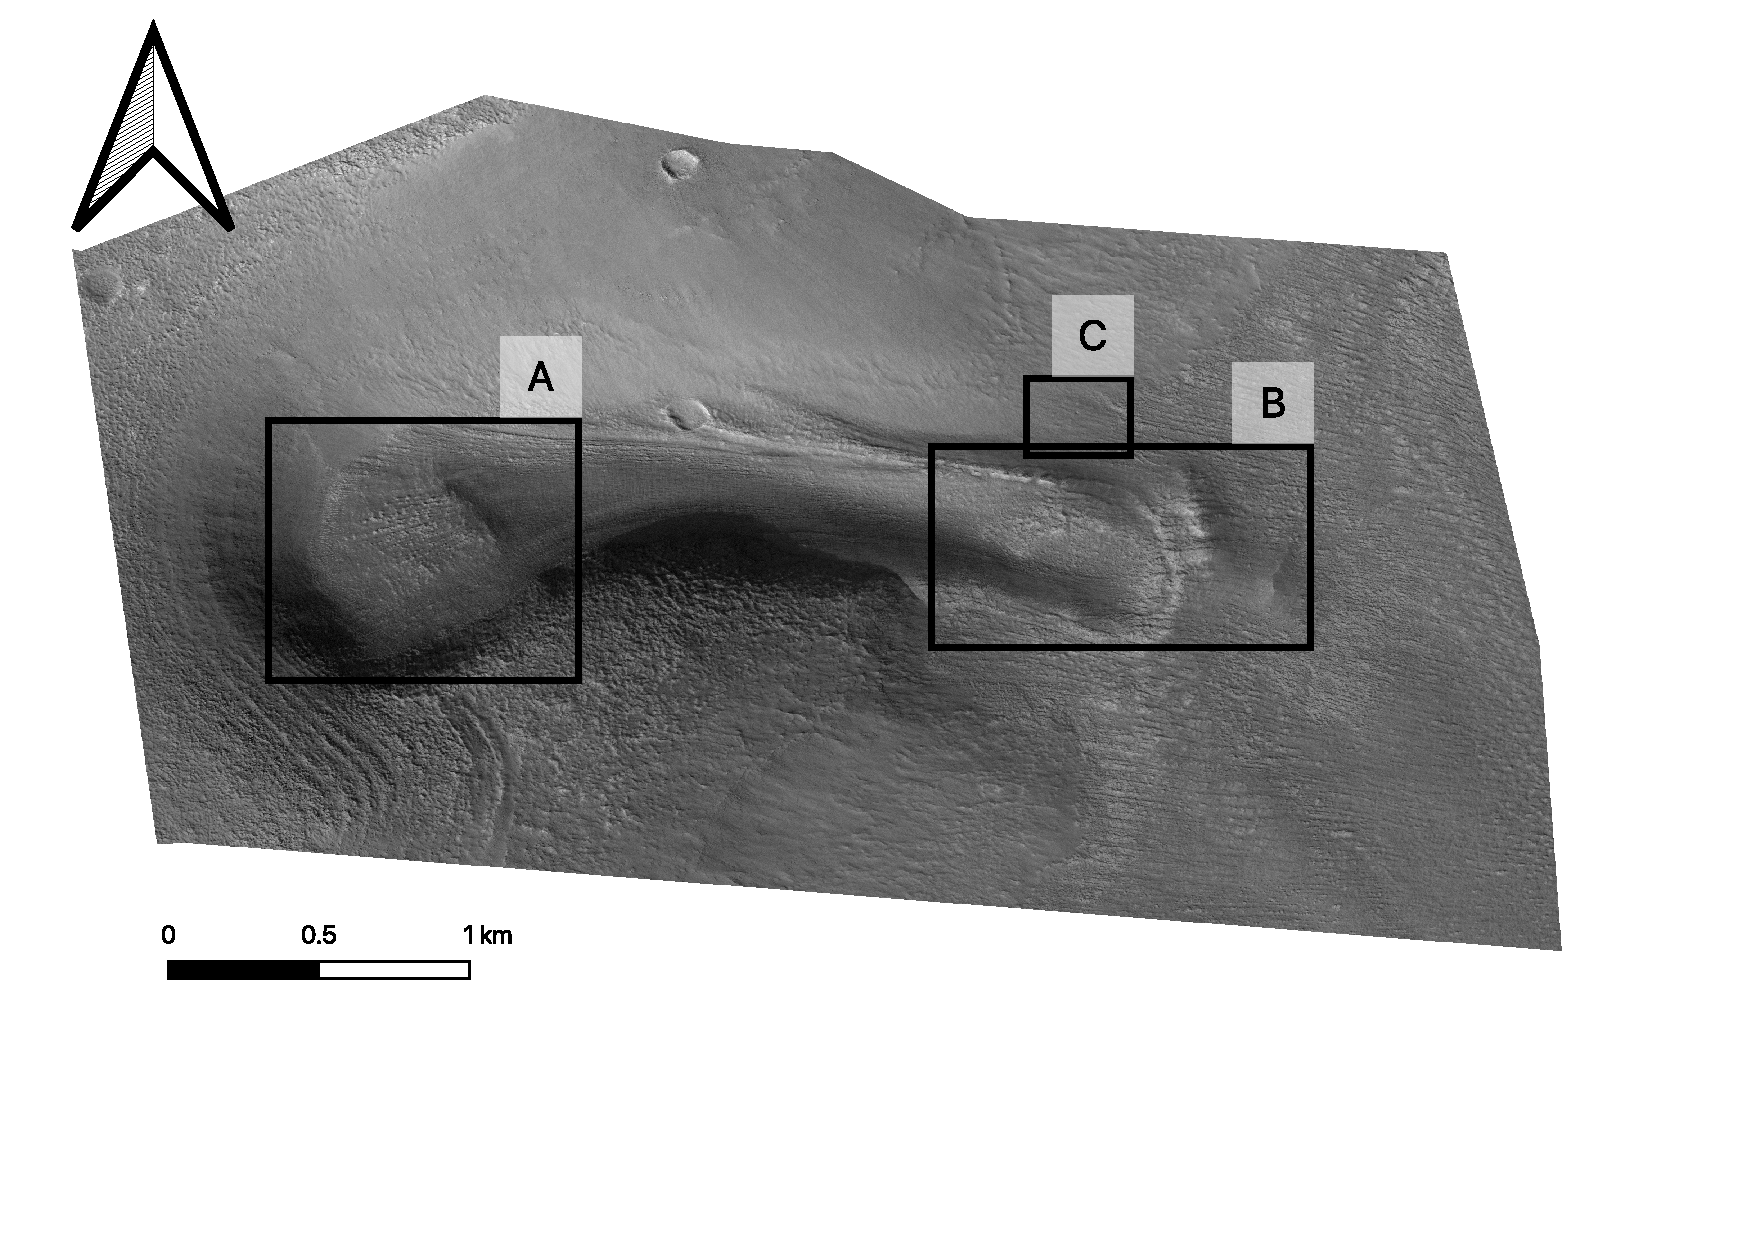
\includegraphics[
        width=\linewidth,
        height=0.65\textheight,
        keepaspectratio
    ]{Figures/Maps/HiRISE_Final_FigsImg.pdf}
    \label{fig:HiRISEOverview_b}
\end{subfigure}

\caption{Overview of alcove feature in NW Ismenius Cavus, mapped using HiRISE data (mapped at $1:2\ 000$ scale).}
\label{fig:HiRISEOverview}

\end{figure}
\end{frame}


\tikzset{
legendunit/.style={
draw=black,
rounded corners=2pt,
minimum width=1.15cm,
minimum height=0.55cm,
font=\scriptsize
},
legendlabel/.style={
align=center,
font=\scriptsize,
text width=2.8cm
}
}

\begin{frame}{Alcove Unit Legend}

\centering

\begin{tikzpicture}[x=2.8cm,y=0.9cm]

%---------------------------------
% HEADERS
%---------------------------------

\node[font=\Large] at (0,0) {Fields};

\node[font=\Large] at (2.5,0)
{Patterned Floor};

%---------------------------------
% FIELDS COLUMN 1
%---------------------------------

\node[legendlabel] at (-0.5,-1)
{smooth field};
\node[legendunit,fill=fieldgreen!20]
at (-0.5,-1.9) {SF};

\node[legendlabel] at (-0.5,-3)
{smooth rubble field};
\node[legendunit,fill=fieldgreen!40]
at (-0.5,-3.9) {SRF};

\node[legendlabel] at (-0.5,-5)
{rough field};
\node[legendunit,fill=fieldgreen!70]
at (-0.5,-5.9) {RF};

%---------------------------------
% FIELDS COLUMN 2
%---------------------------------

\node[legendlabel] at (0.7,-1)
{smooth scarp};
\node[legendunit,fill=scarporange!20]
at (0.7,-1.9) {SS};

\node[legendlabel] at (0.7,-3)
{transverse longitudinal\\surface structure};
\node[legendunit,fill=fieldgreen!55]
at (0.7,-3.9) {TLSS};

%---------------------------------
% PATTERNED FLOOR
%---------------------------------

\node[legendlabel] at (2.5,-1)
{fine polygonal field};
\node[legendunit,fill=risepurple!25]
at (2.5,-1.9) {FP};

\node[legendlabel] at (2.5,-3)
{rubble fine polygonal\\field};
\node[legendunit,fill=risepurple!45]
at (2.5,-3.9) {RFP};

\node[legendlabel] at (2.5,-5)
{ribbed field};
\node[legendunit,fill=risepurple!65]
at (2.5,-5.9) {RBF};

\end{tikzpicture}

\end{frame}

\begin{frame}{HiRISE Unit Legend: Ridge Systems}

\centering

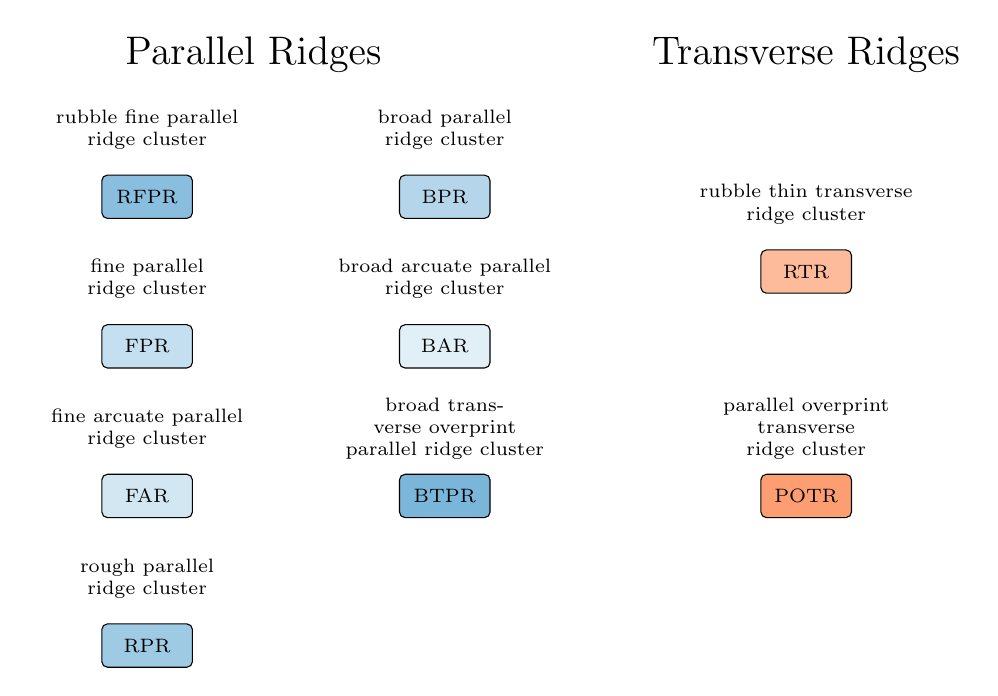
\begin{tikzpicture}[x=2.7cm,y=0.95cm]

\tikzset{
legendunit/.style={
draw=black,
rounded corners=2pt,
minimum width=1.15cm,
minimum height=0.55cm,
font=\scriptsize
},
legendlabel/.style={
align=center,
font=\scriptsize,
text width=2.8cm
}
}

%--------------------------------------------------
% HEADERS
%--------------------------------------------------

\node[font=\Large] at (0,0)
{Parallel Ridges};

\node[font=\Large] at (2.6,0)
{Transverse Ridges};

%--------------------------------------------------
% PARALLEL RIDGES COLUMN 1
%--------------------------------------------------

\node[legendlabel] at (-0.5,-1)
{rubble fine parallel\\ridge cluster};
\node[legendunit,fill=flowblue!80]
at (-0.5,-1.9) {RFPR};

\node[legendlabel] at (-0.5,-3)
{fine parallel\\ridge cluster};
\node[legendunit,fill=flowblue!40]
at (-0.5,-3.9) {FPR};

\node[legendlabel] at (-0.5,-5)
{fine arcuate parallel\\ridge cluster};
\node[legendunit,fill=flowblue!30]
at (-0.5,-5.9) {FAR};

\node[legendlabel] at (-0.5,-7)
{rough parallel\\ridge cluster};
\node[legendunit,fill=flowblue!65]
at (-0.5,-7.9) {RPR};

%--------------------------------------------------
% PARALLEL RIDGES COLUMN 2
%--------------------------------------------------

\node[legendlabel] at (0.9,-1)
{broad parallel\\ridge cluster};
\node[legendunit,fill=flowblue!50]
at (0.9,-1.9) {BPR};

\node[legendlabel] at (0.9,-3)
{broad arcuate parallel\\ridge cluster};
\node[legendunit,fill=flowblue!20]
at (0.9,-3.9) {BAR};

\node[legendlabel] at (0.9,-5)
{broad transverse overprint\\parallel ridge cluster};
\node[legendunit,fill=flowblue!90]
at (0.9,-5.9) {BTPR};

%--------------------------------------------------
% TRANSVERSE RIDGES
%--------------------------------------------------

\node[legendlabel] at (2.6,-2)
{rubble thin transverse\\ridge cluster};
\node[legendunit,fill=scarporange!60]
at (2.6,-2.9) {RTR};

\node[legendlabel] at (2.6,-5)
{parallel overprint\\transverse ridge cluster};
\node[legendunit,fill=scarporange!85]
at (2.6,-5.9) {POTR};

\end{tikzpicture}

\end{frame}
\againframe{Corrie}
\begin{frame}{Regions of Interest}

\begin{figure}
\centering

\begin{subfigure}{0.48\textwidth}
    \centering
    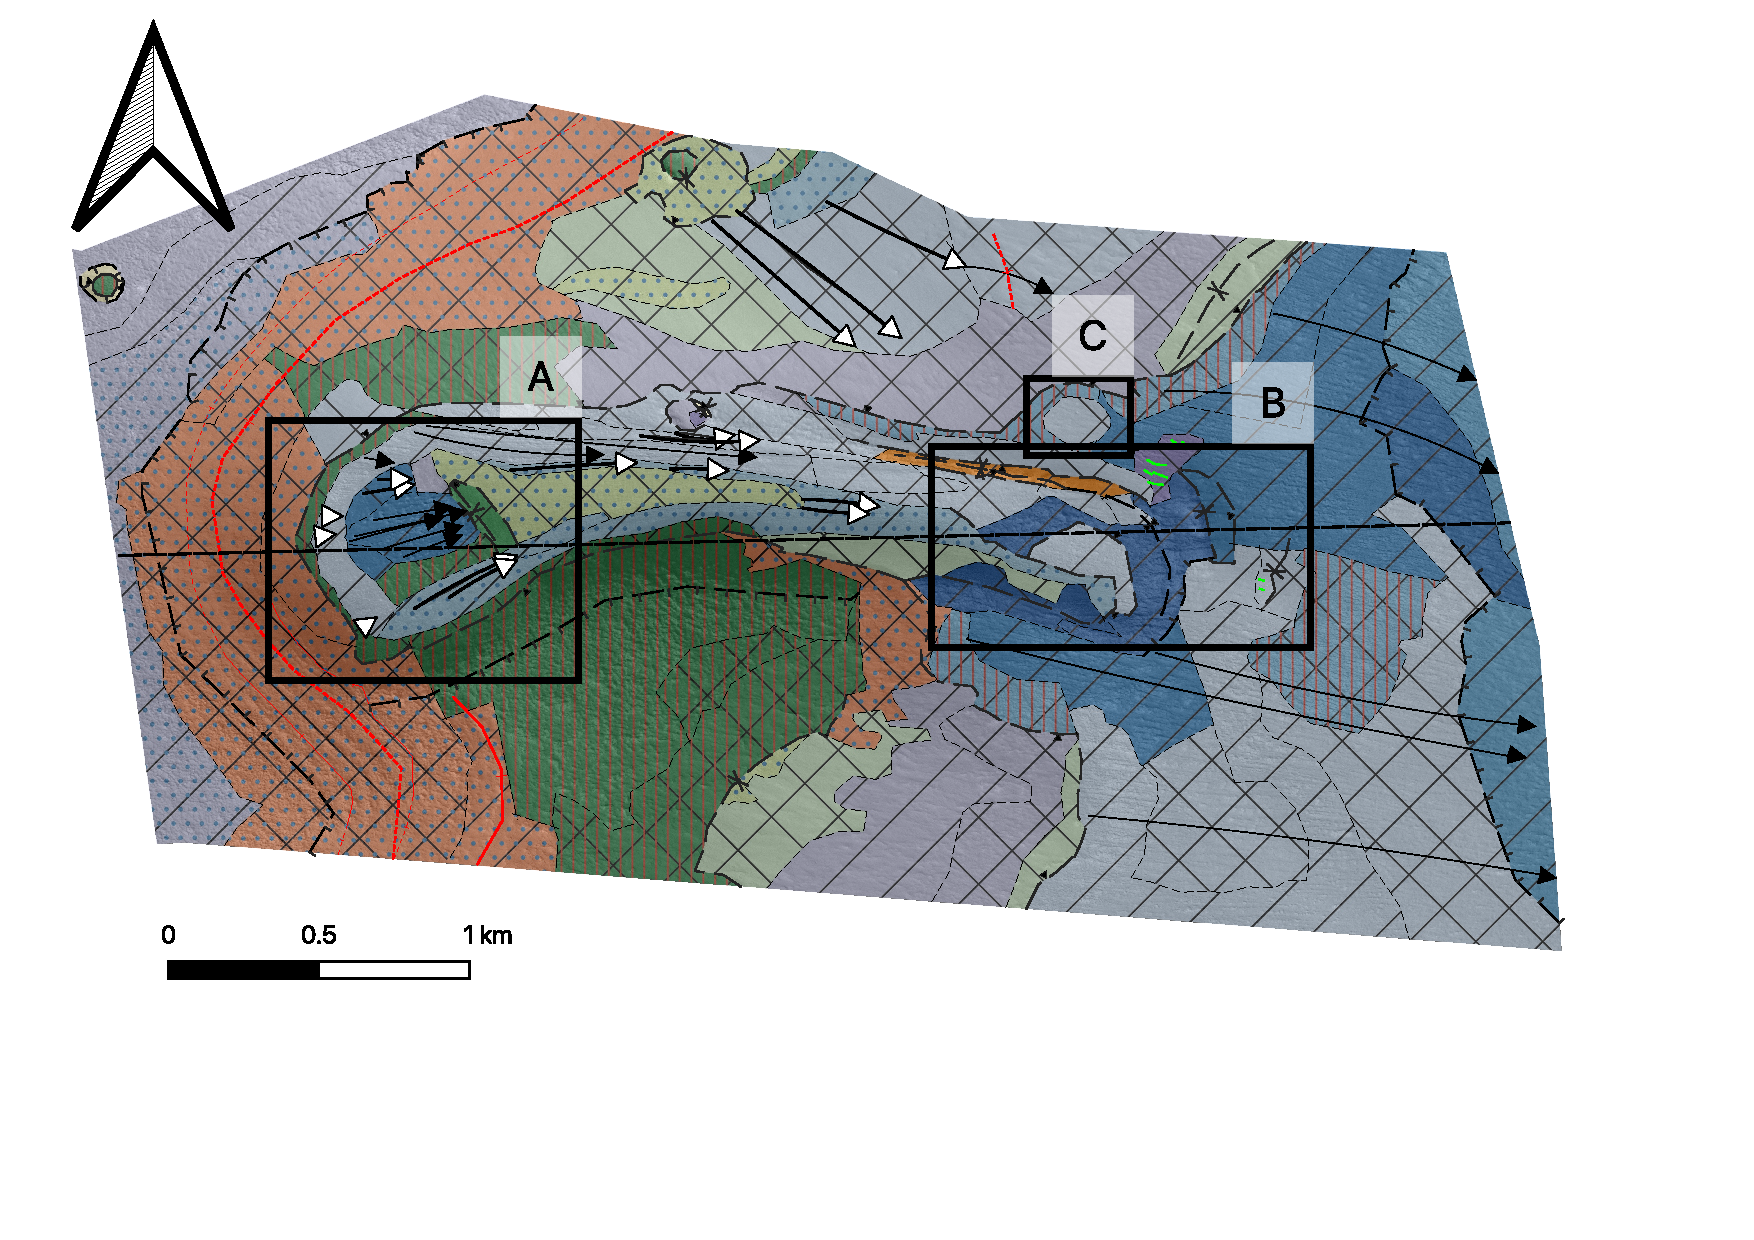
\includegraphics[
        width=\linewidth,
        height=0.65\textheight,
        keepaspectratio
    ]{Figures/Maps/HiRISE_Final_FigsMap.pdf}
    \label{fig:HiRISEFinal_a}
\end{subfigure}
\hfill
\begin{subfigure}{0.48\textwidth}
    \centering
    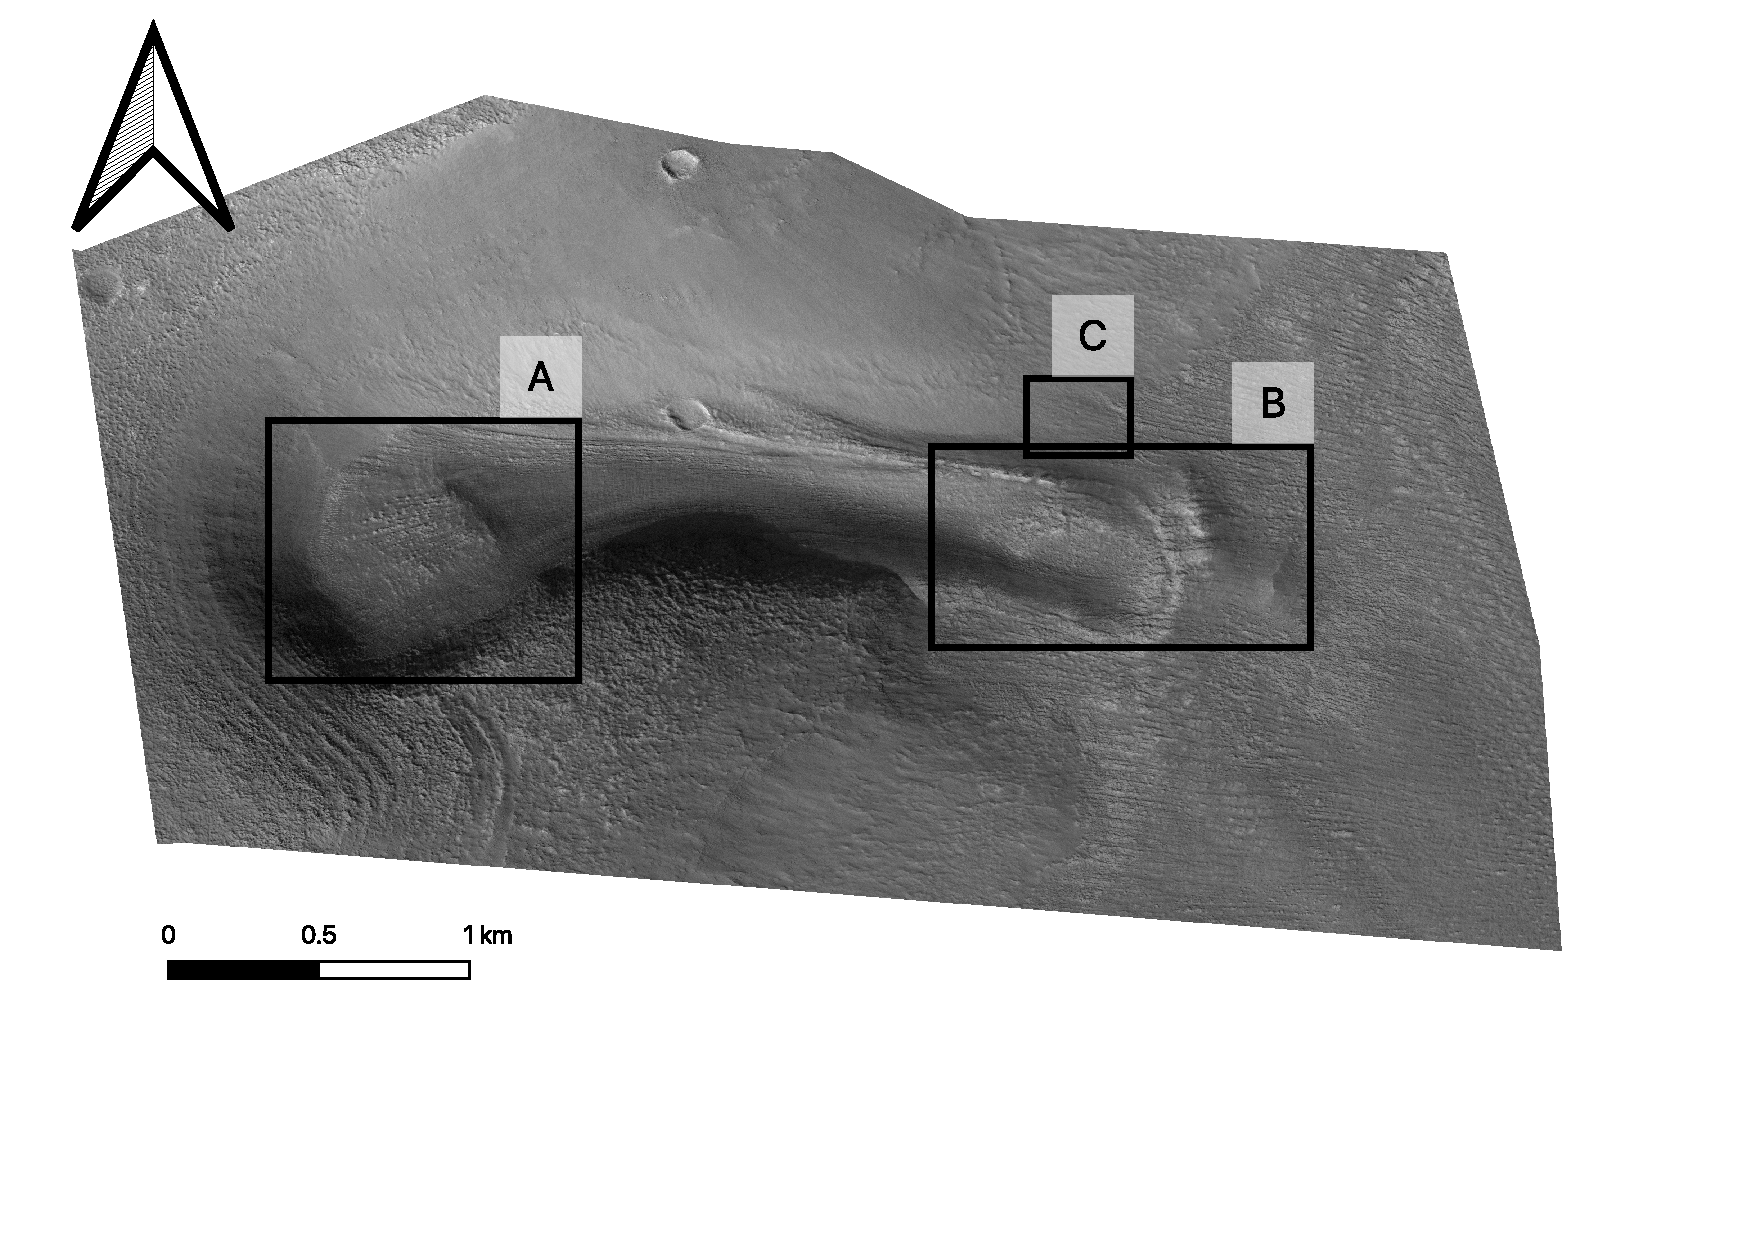
\includegraphics[
        width=\linewidth,
        height=0.65\textheight,
        keepaspectratio
    ]{Figures/Maps/HiRISE_Final_FigsImg.pdf}
    \label{fig:HiRISEFinal_b}
\end{subfigure}

\caption{Overview of alcove feature in NW Ismenius Cavus, mapped using HiRISE data. Inserts are highlighted (to be shown in alphabetical order).}
\label{fig:HiRISEFinal}

\end{figure}

\end{frame}

\begin{frame}{Headwall}

\begin{figure}
\centering

\begin{subfigure}{0.48\textwidth}
    \centering
    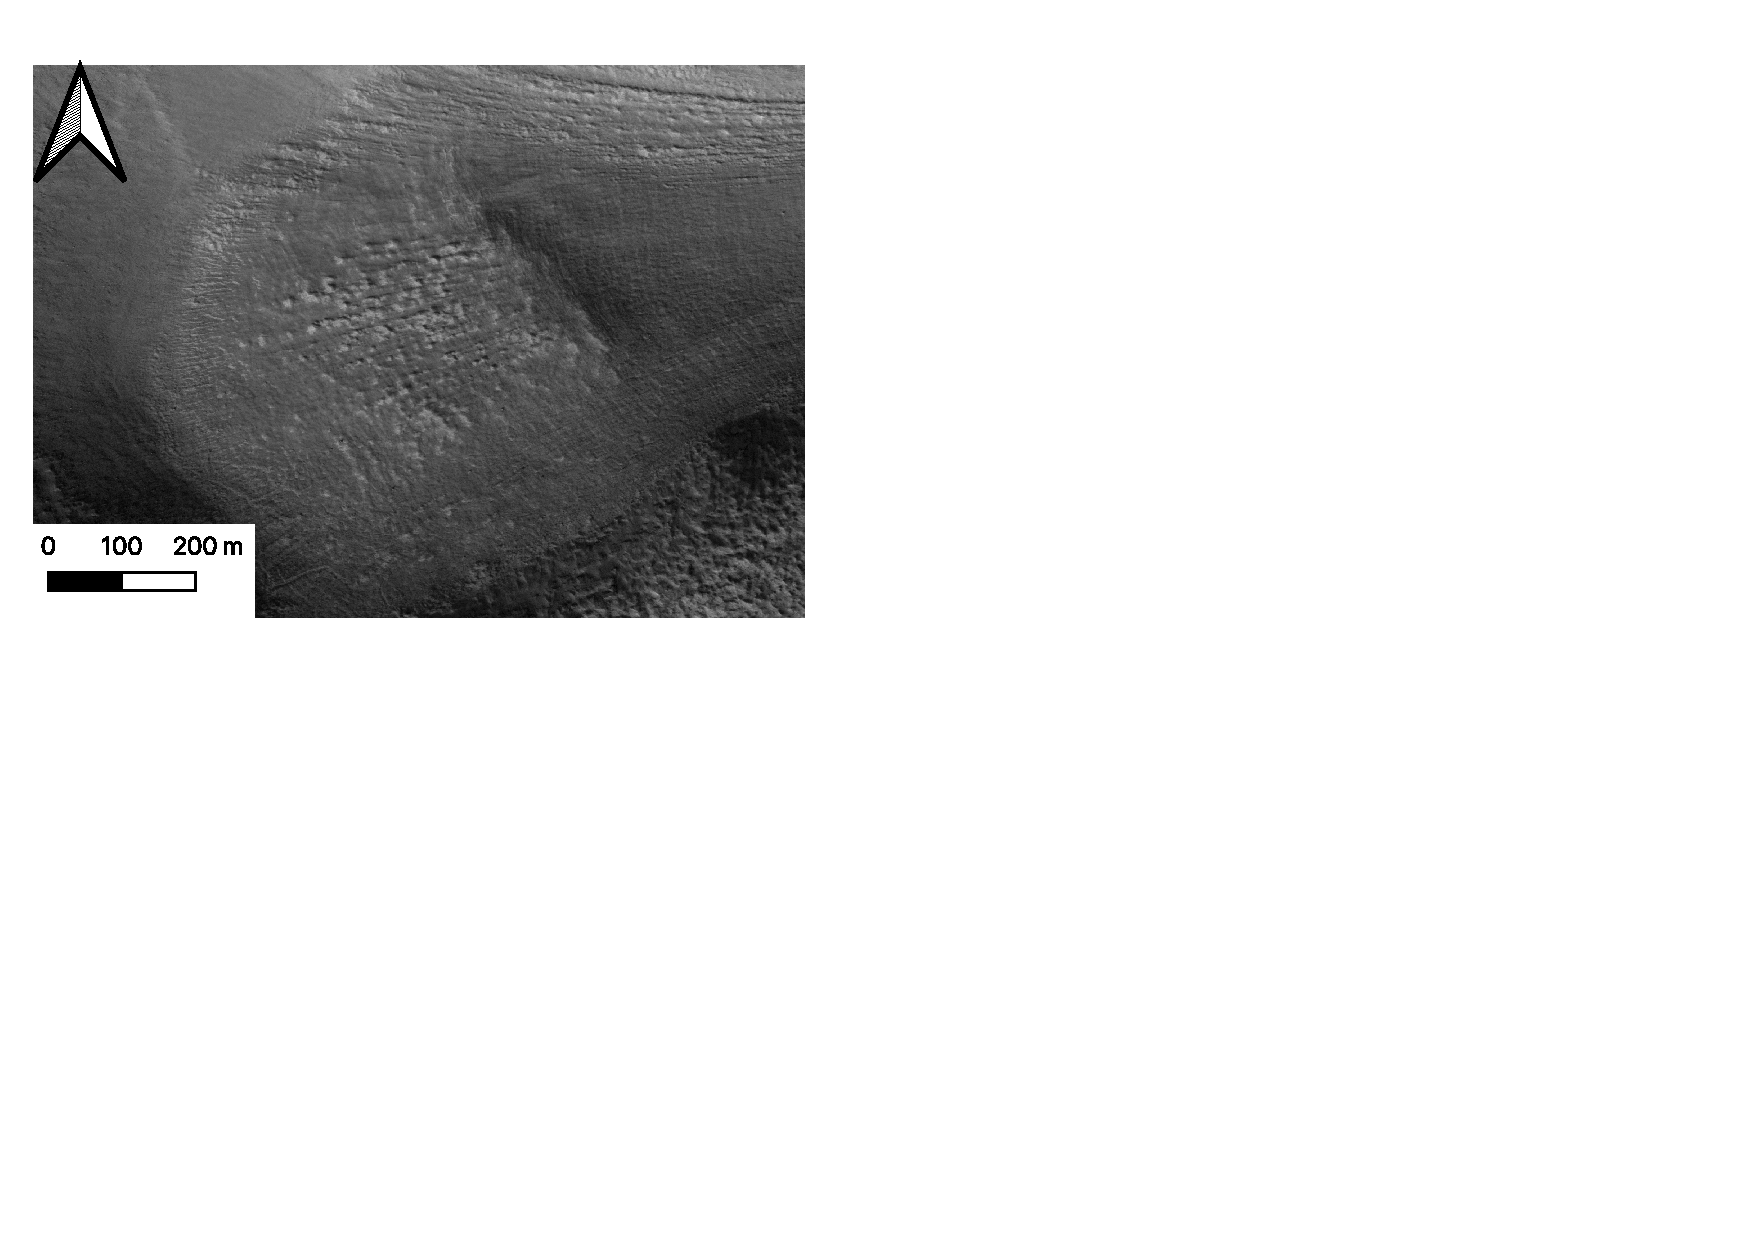
\includegraphics[
        width=\linewidth,
        height=0.65\textheight,
        keepaspectratio
    ]{Figures/HiRISE/Headwall_Img.pdf}
    \label{fig:Headwall_a}
\end{subfigure}
\hfill
\begin{subfigure}{0.48\textwidth}
    \centering
    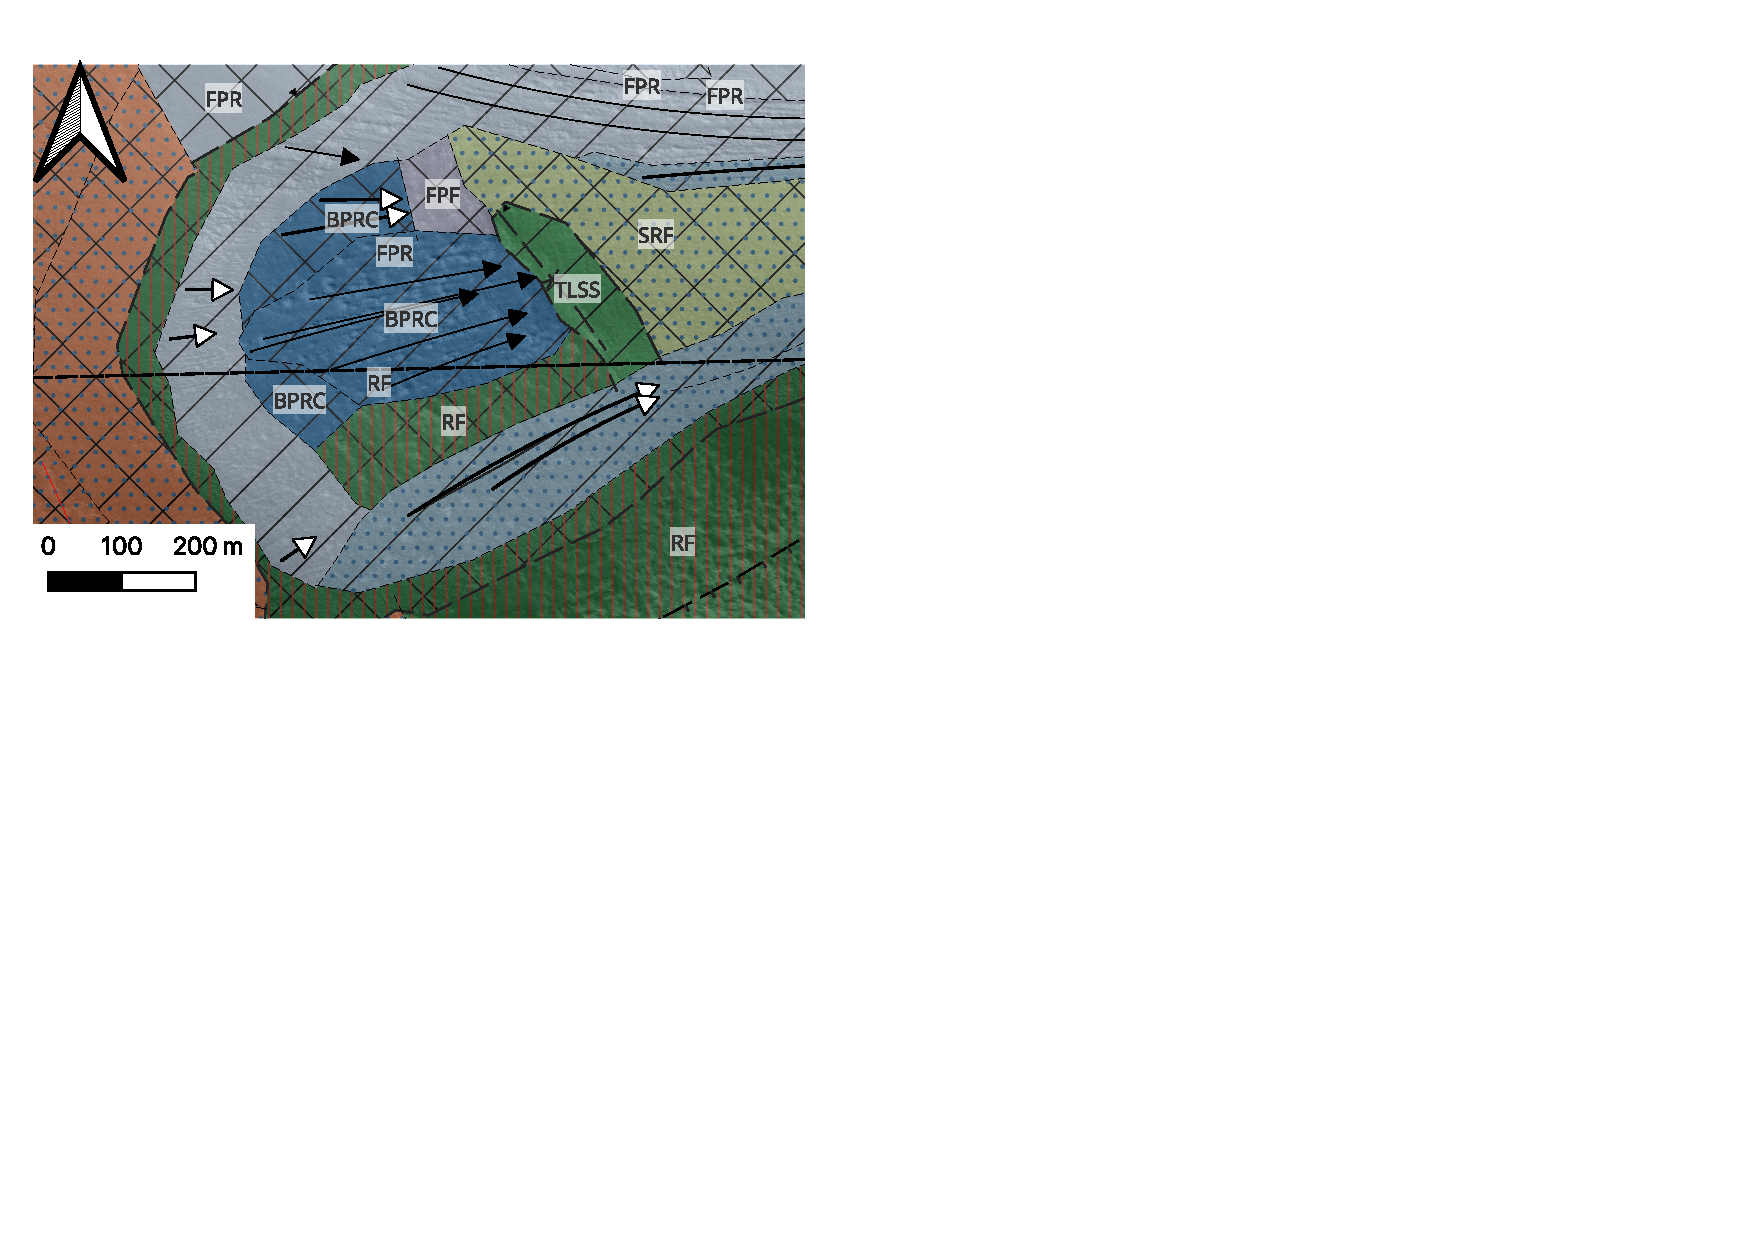
\includegraphics[
        width=\linewidth,
        height=0.65\textheight,
        keepaspectratio
    ]{Figures/HiRISE/Headwall_Map.pdf}
    \label{fig:Headwall_b}
\end{subfigure}

\caption{Headwall, showing linear flow features, rubble and a levee-type feature ($290 \mathrm{\ m} \times 95 \mathrm{\ m}$; centred at $34.62321^{\circ}$N, $16.79698^{\circ}$E) }
\label{fig:Headwall}

\end{figure}

\end{frame}

\begin{frame}{Apron Foot}

\begin{figure}
\centering

\begin{subfigure}{0.48\textwidth}
    \centering
    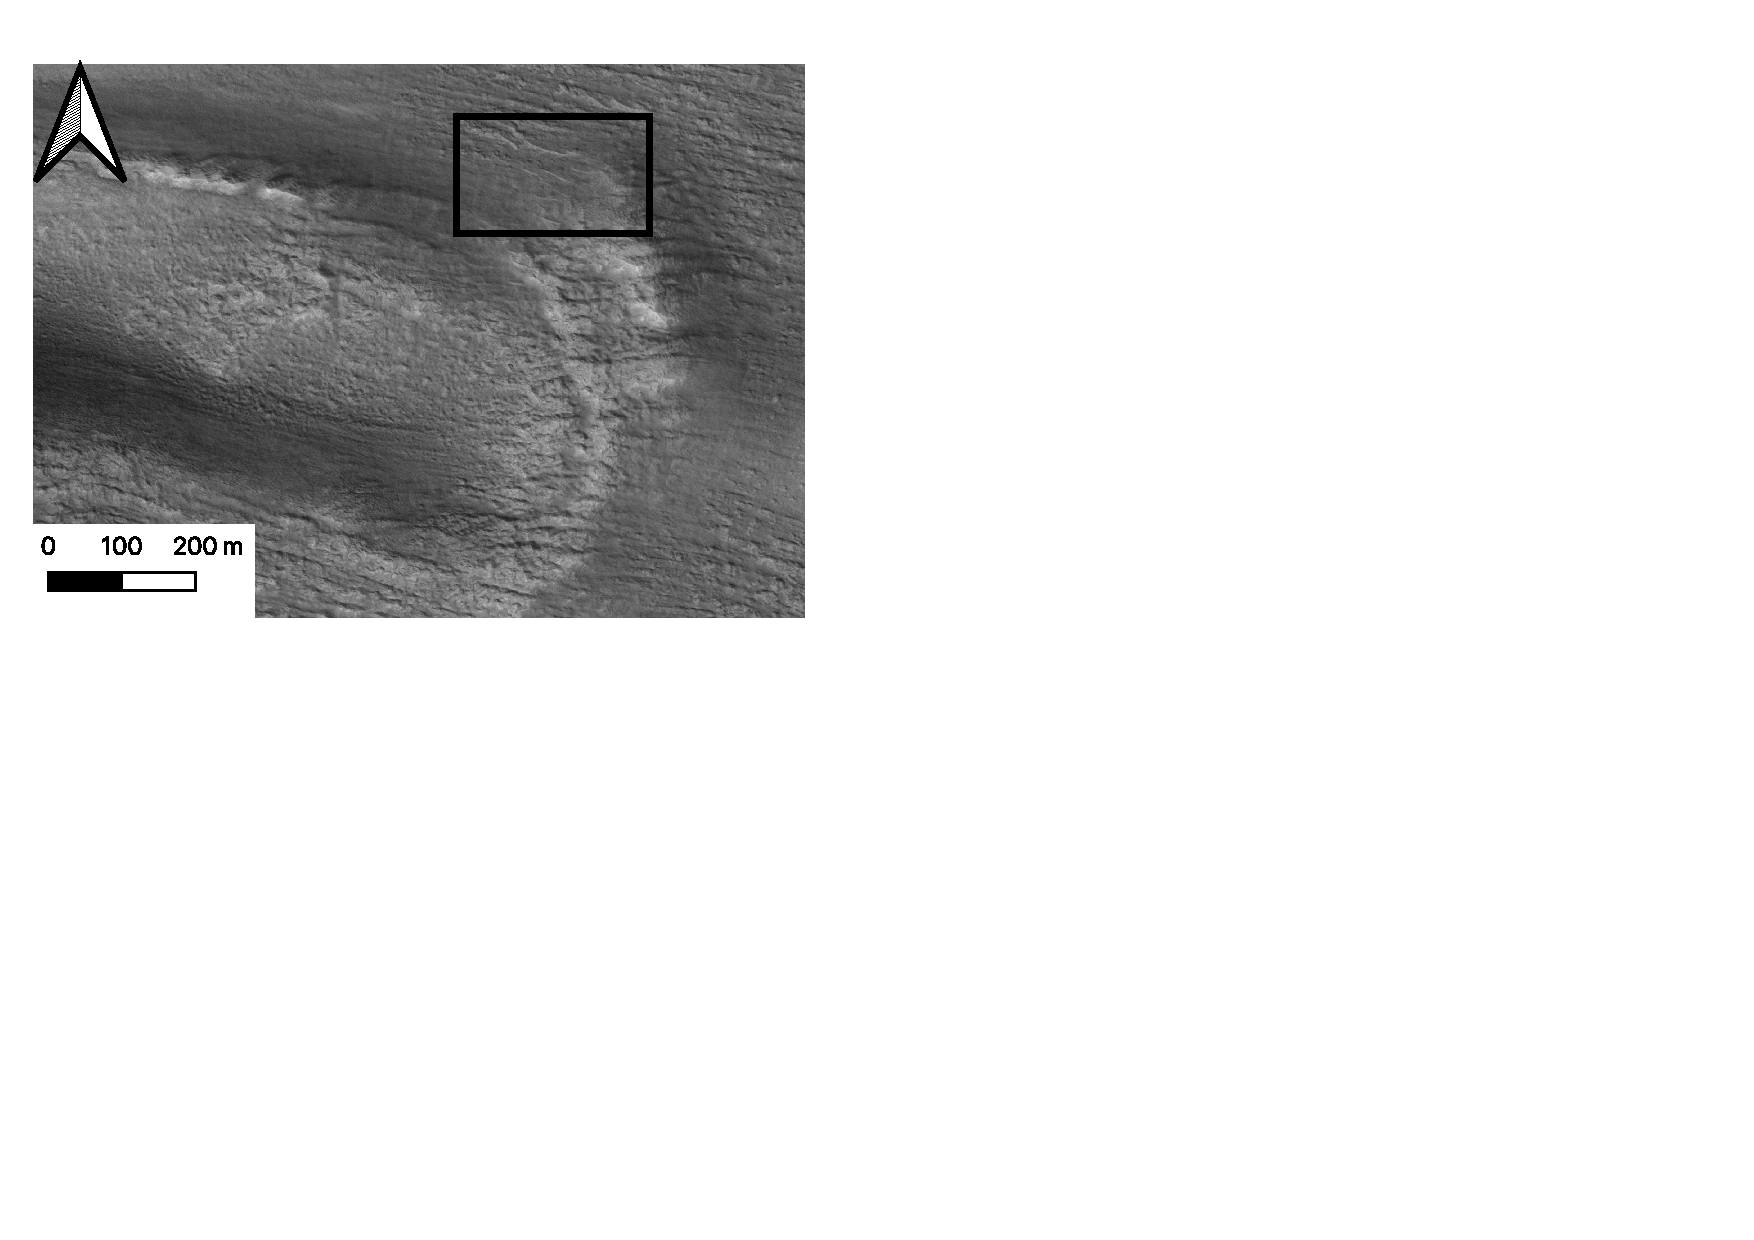
\includegraphics[
        width=\linewidth,
        height=0.65\textheight,
        keepaspectratio
    ]{Figures/HiRISE/Foot_Img.pdf}
    \label{fig:Foot_a}
\end{subfigure}
\hfill
\begin{subfigure}{0.48\textwidth}
    \centering
    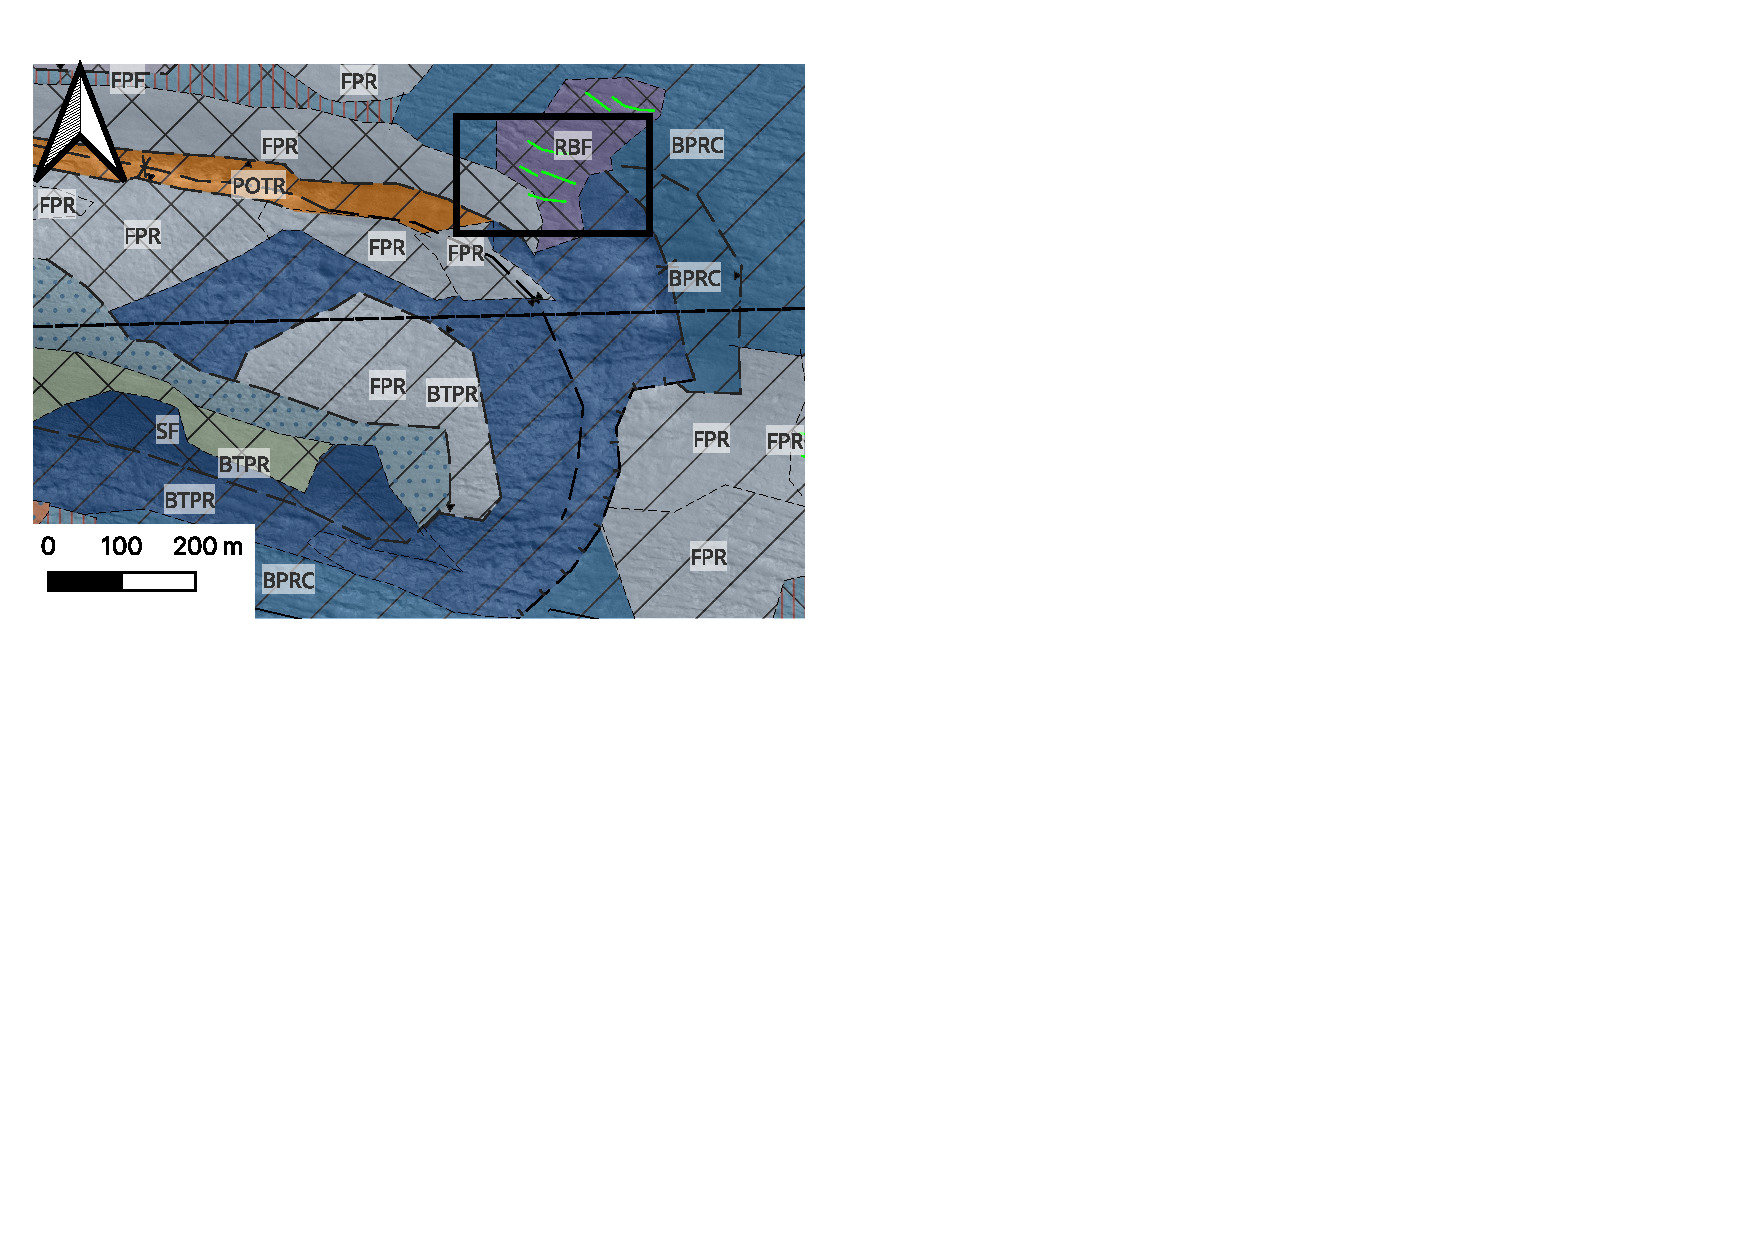
\includegraphics[
        width=\linewidth,
        height=0.65\textheight,
        keepaspectratio
    ]{Figures/HiRISE/Foot_Map.pdf}
    \label{fig:Foot_b}
\end{subfigure}

\caption{The apron foot. Note the rise and transverse-overprinted ridges (centred at $34.62301^{\circ}$N, $16.83755^{\circ}$E).}
\label{fig:Foot}
\end{figure}
\end{frame}

\begin{frame}{Aeolian Modification}

\begin{figure}
\centering

\begin{subfigure}{0.48\textwidth}
    \centering
    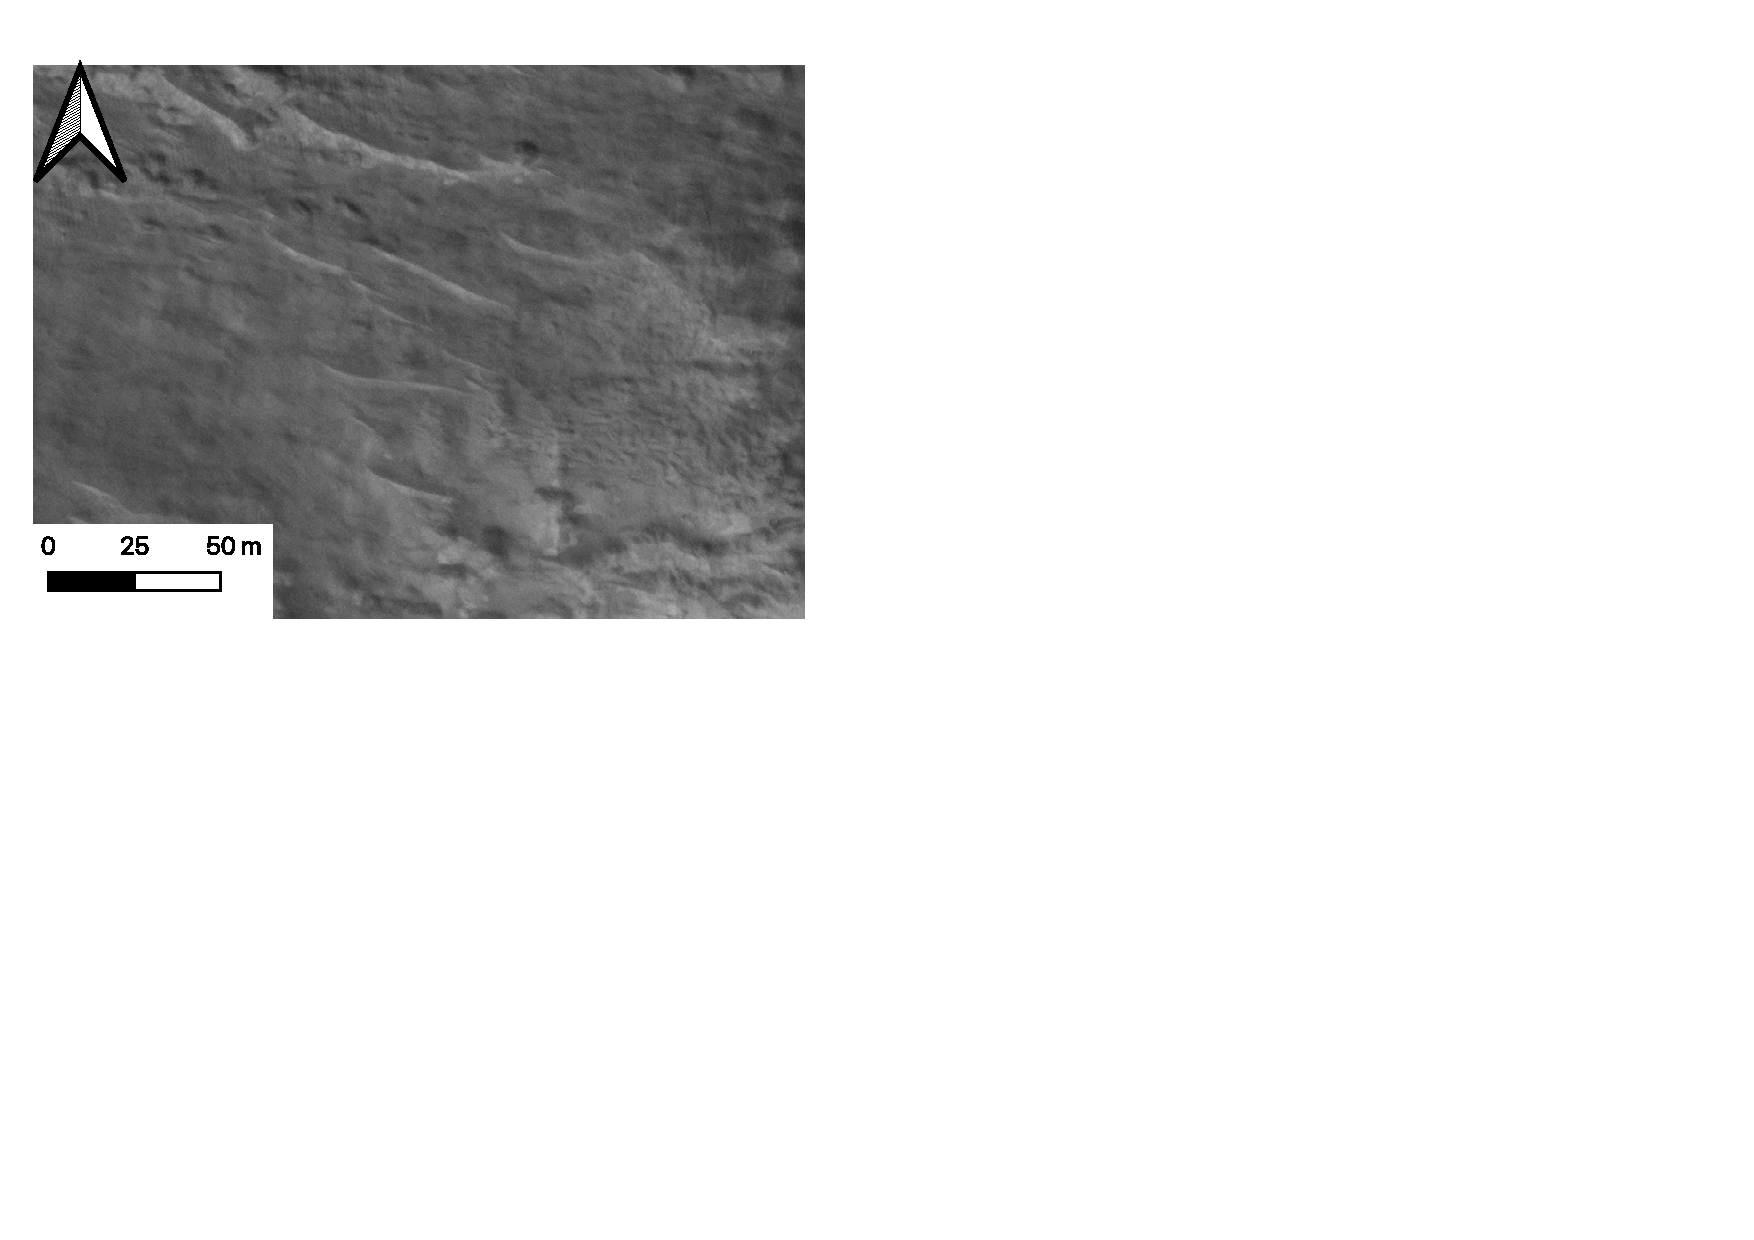
\includegraphics[
        width=\linewidth,
        height=0.65\textheight,
        keepaspectratio
    ]{Figures/HiRISE/Ripples_Img.pdf}
    \label{fig:Ripples_a}
\end{subfigure}
\hfill
\begin{subfigure}{0.48\textwidth}
    \centering
    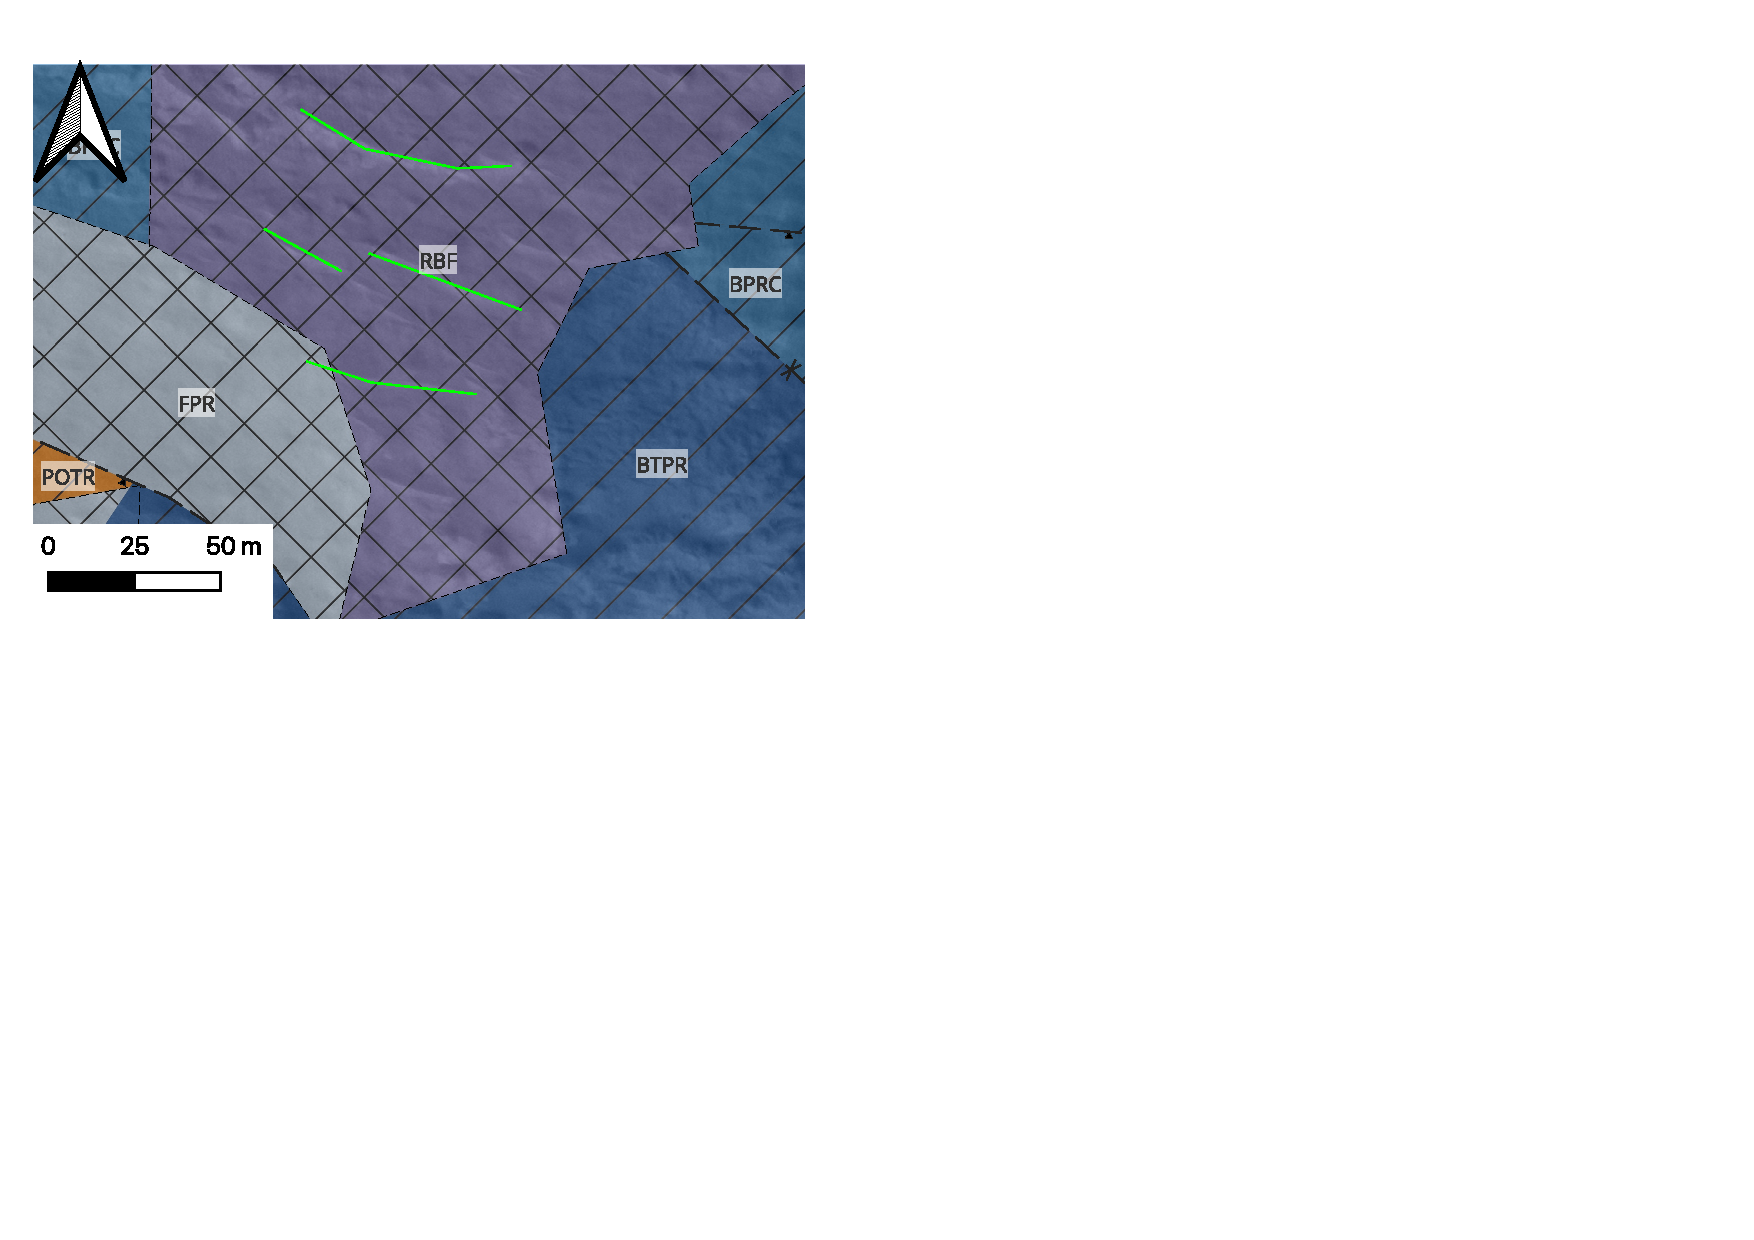
\includegraphics[
        width=\linewidth,
        height=0.65\textheight,
        keepaspectratio
    ]{Figures/HiRISE/Ripples_Map.pdf}
    \label{fig:Ripples_b}
\end{subfigure}

\caption{Rib-shaped lineations indicating aeolian modification (centred at $34.62723^{\circ}$N, $16.83848^{\circ}$E).}
\label{fig:Ripples}
\end{figure}
\end{frame}

\begin{frame}{Highly Modified Crater}

\begin{figure}
\centering

\begin{subfigure}{0.48\textwidth}
    \centering
    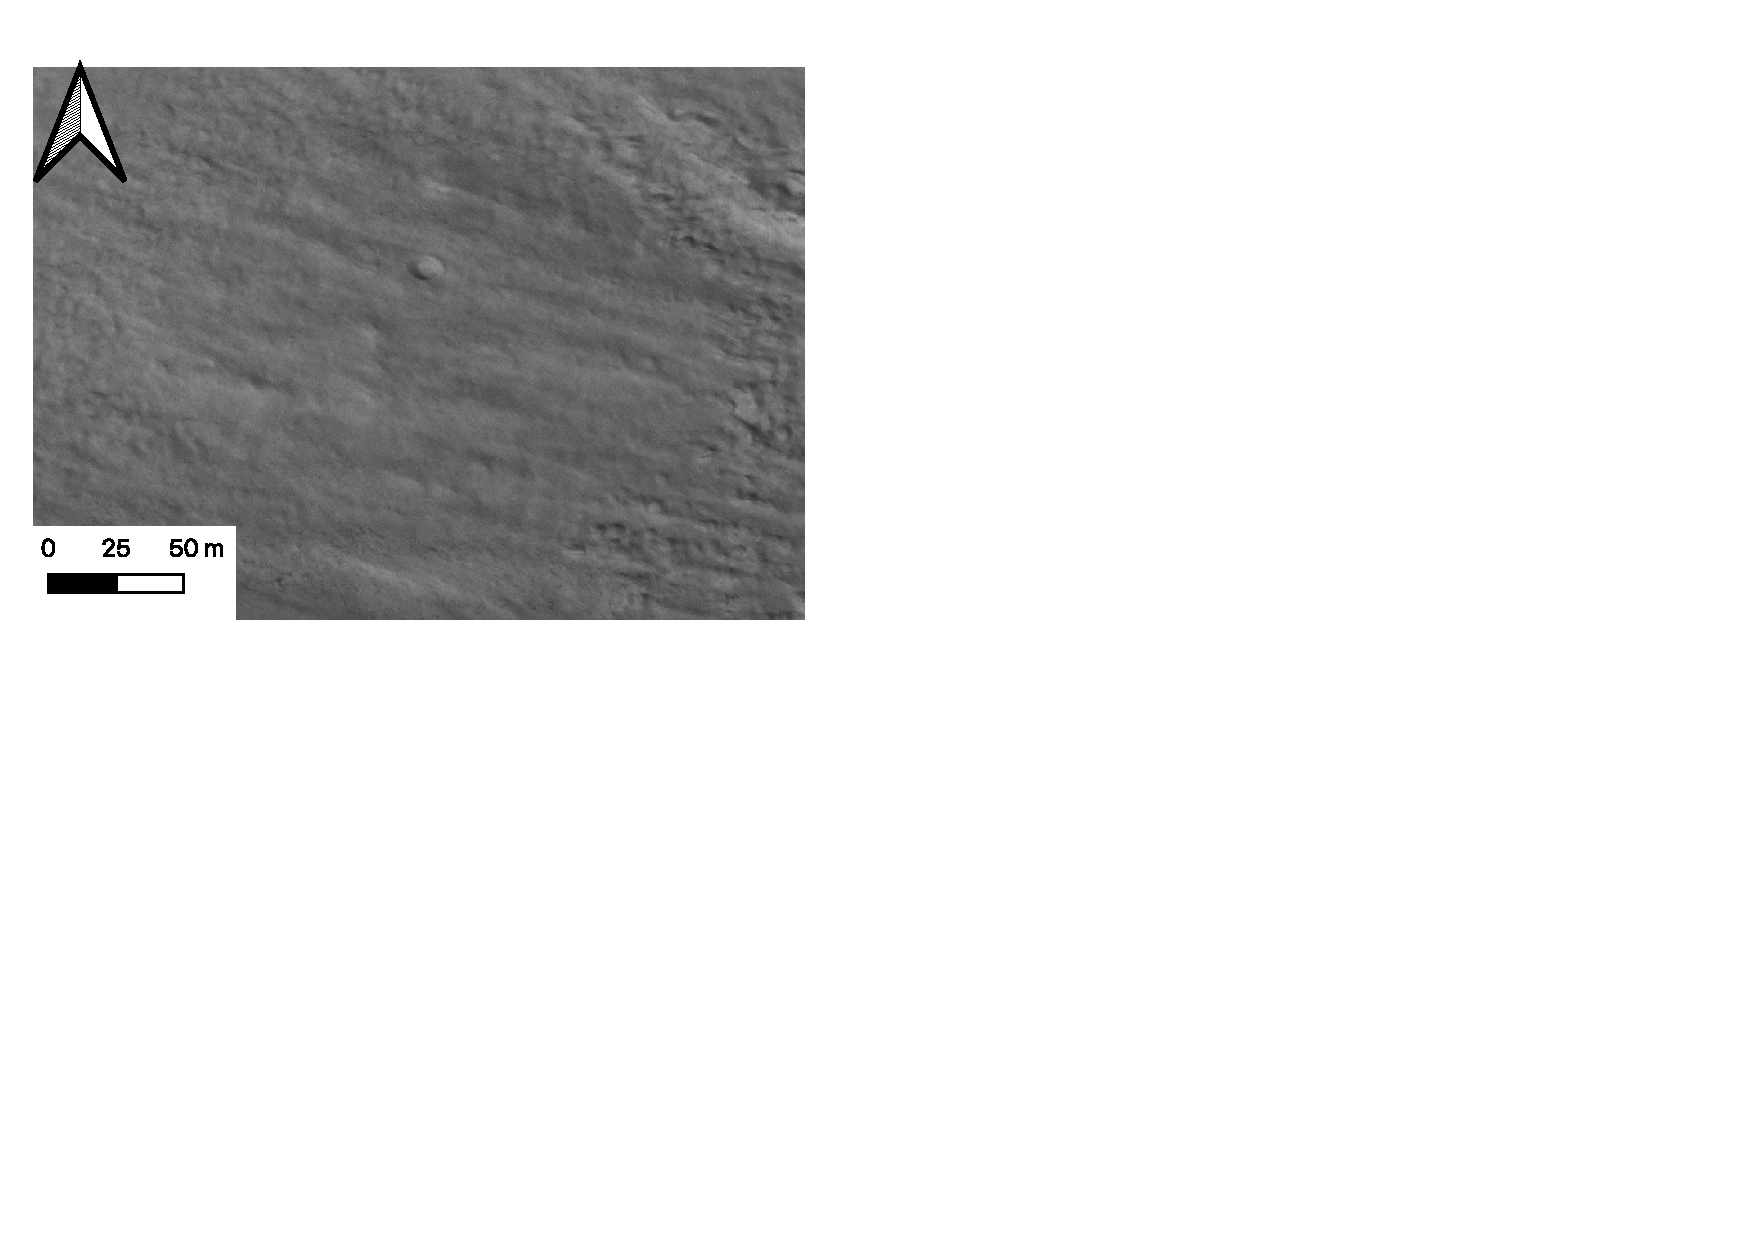
\includegraphics[
        width=\linewidth,
        height=0.65\textheight,
        keepaspectratio
    ]{Figures/HiRISE/GhostCrater_Img.pdf}
    \label{fig:GhostCrater_a}
\end{subfigure}
\hfill
\begin{subfigure}{0.48\textwidth}
    \centering
    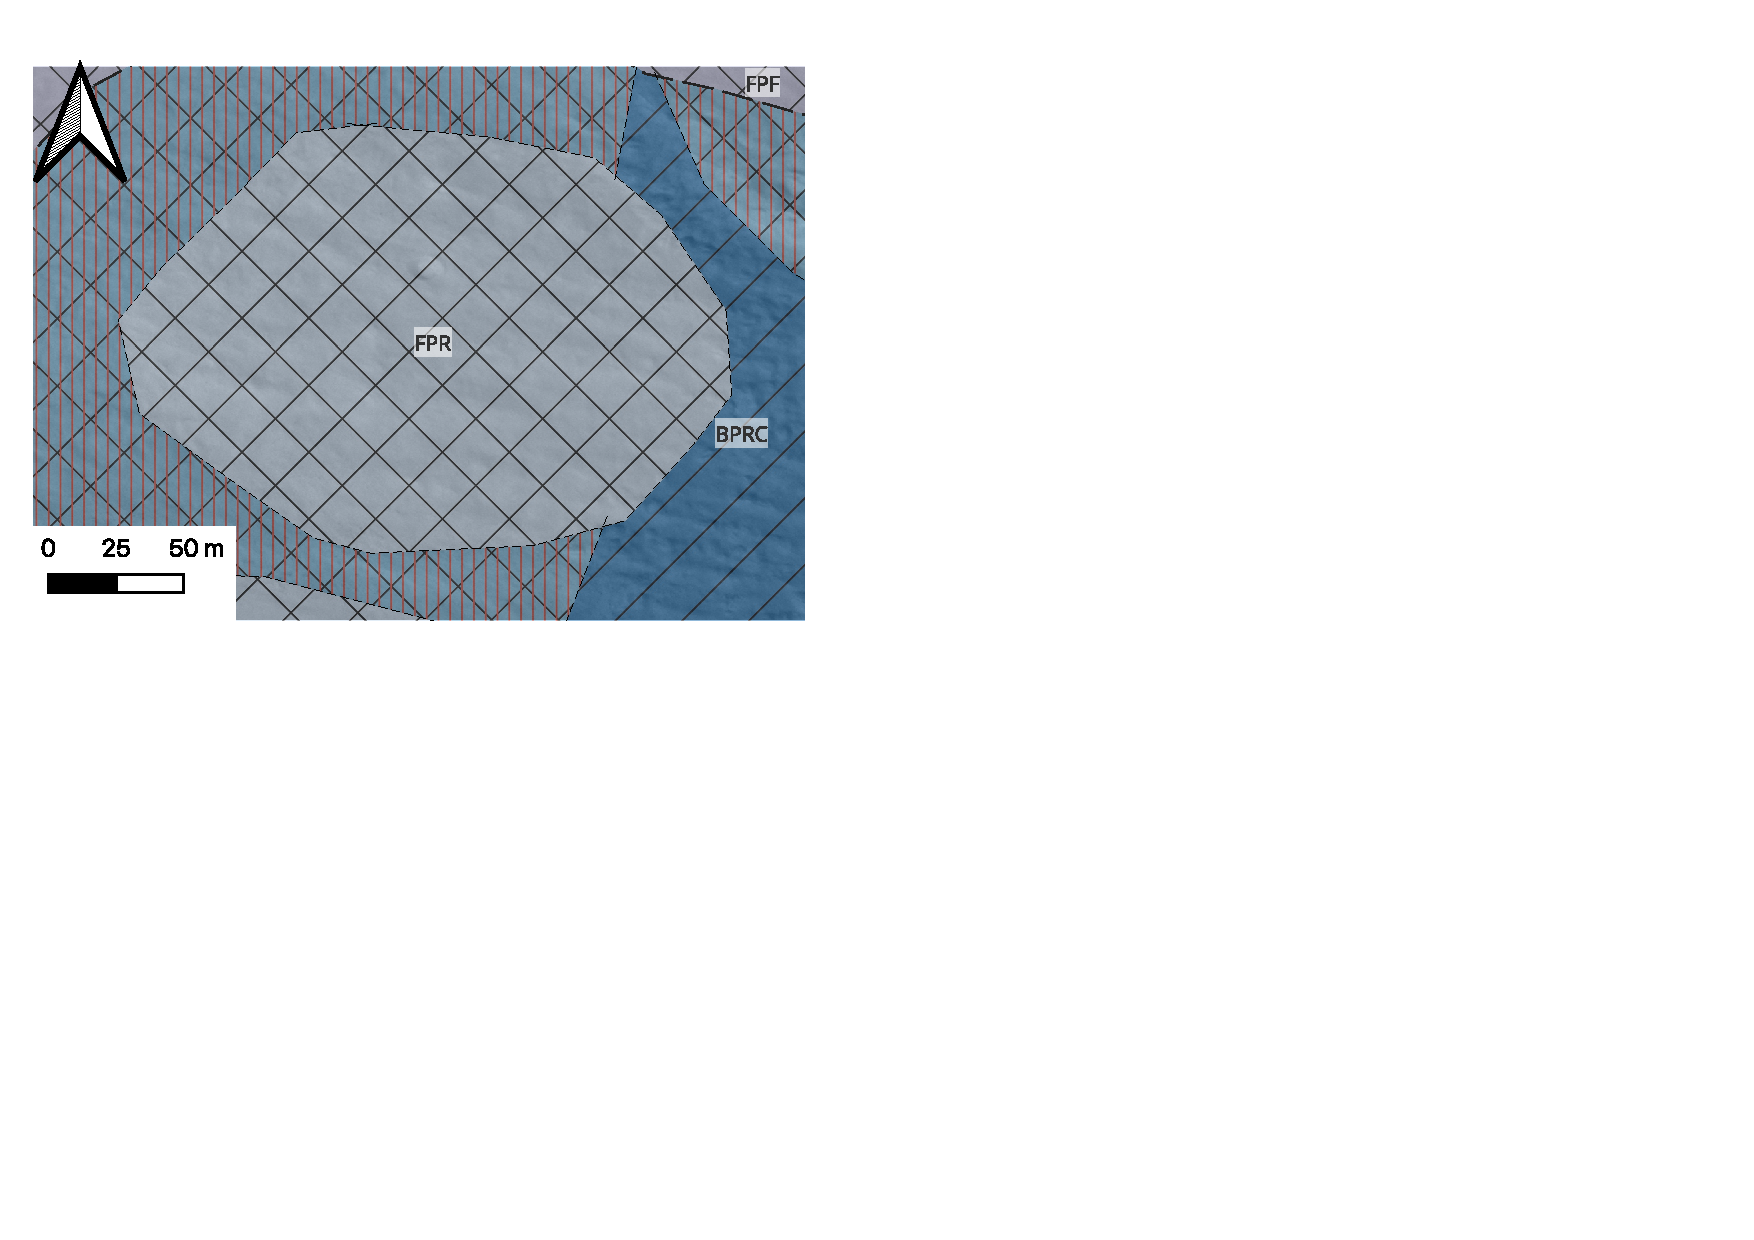
\includegraphics[
        width=\linewidth,
        height=0.65\textheight,
        keepaspectratio
    ]{Figures/HiRISE/GhostCrater_Map.pdf}
    \label{fig:GhostCrater_b}
\end{subfigure}

\caption{Circular smooth surface, suggestive of a ghost crater (centred at $34.62873^{\circ}$N, $16.83217^{\circ}$E).}
\label{fig:GhostCrater}

\end{figure}

\end{frame}


\begin{frame}{Stratigraphic Correlations of Alcove Units}

\centering

\resizebox{\textwidth}{!}{
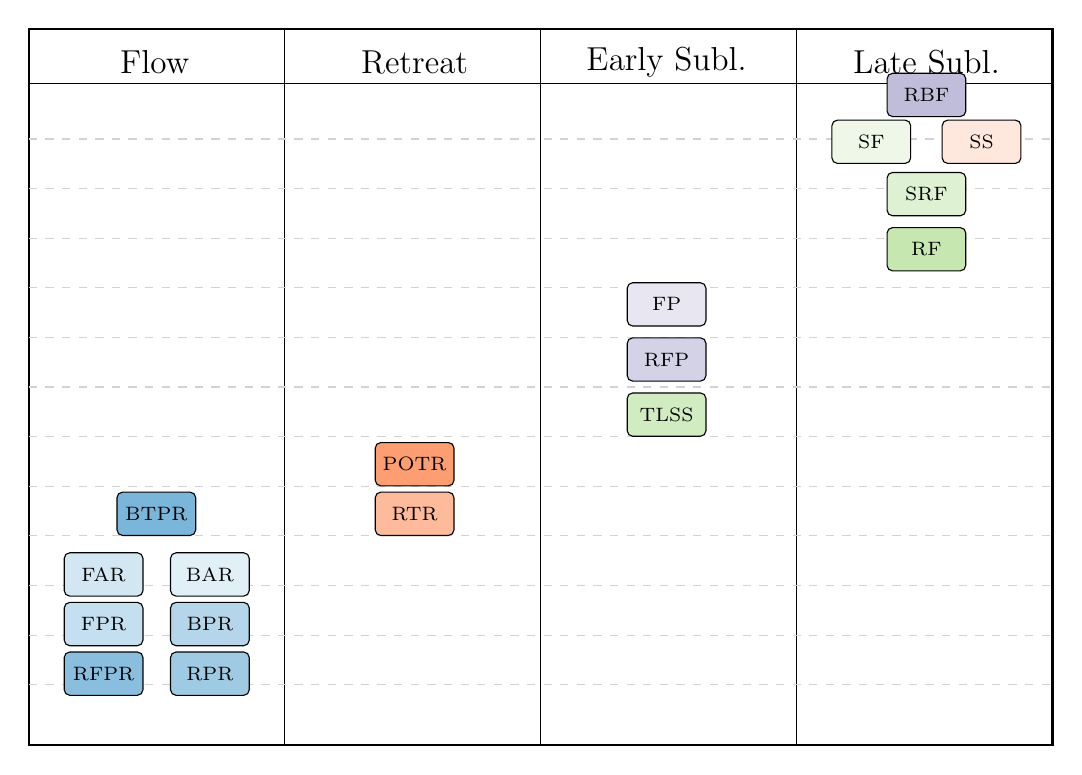
\begin{tikzpicture}[x=1cm,y=0.7cm]

%--------------------------------------------------
% STYLES
%--------------------------------------------------

\tikzset{
stratunit/.style={
draw=black,
rounded corners=2pt,
minimum width=1.0cm,
minimum height=0.55cm,
font=\scriptsize,
inner sep=2pt
}
}

%--------------------------------------------------
% FRAME
%--------------------------------------------------

\draw[line width=0.8pt] (0,0) rectangle (13,13);

\draw (3.25,0)--(3.25,13);
\draw (6.50,0)--(6.50,13);
\draw (9.75,0)--(9.75,13);

\draw (0,12)--(13,12);

%--------------------------------------------------
% HEADERS
%--------------------------------------------------

\node[font=\large] at (1.6,12.40)
{Flow};

\node[font=\large] at (4.9,12.40)
{Retreat};

\node[font=\large] at (8.10,12.40)
{Early Subl.};

\node[font=\large] at (11.40,12.40)
{Late Subl.};

%--------------------------------------------------
% GUIDES
%--------------------------------------------------

\foreach \y in {1.1,2.0,2.9,3.8,4.7,5.6,6.5,7.4,8.3,9.2,10.1,11.0}
{
\draw[dashed,gray!35]
(0,\y)--(13,\y);
}

%--------------------------------------------------
% FLOW
%--------------------------------------------------

\node[stratunit,fill=flowblue!80]
at (0.95,1.30)
{RFPR};

\node[stratunit,fill=flowblue!65]
at (2.30,1.30)
{RPR};

\node[stratunit,fill=flowblue!40]
at (0.95,2.20)
{FPR};

\node[stratunit,fill=flowblue!50]
at (2.30,2.20)
{BPR};

\node[stratunit,fill=flowblue!30]
at (0.95,3.10)
{FAR};

\node[stratunit,fill=flowblue!20]
at (2.30,3.10)
{BAR};

\node[stratunit,fill=flowblue!90]
at (1.62,4.20)
{BTPR};

%--------------------------------------------------
% RETREAT
%--------------------------------------------------

\node[stratunit,fill=scarporange!60]
at (4.90,4.20)
{RTR};

\node[stratunit,fill=scarporange!85]
at (4.90,5.10)
{POTR};

%--------------------------------------------------
% EARLY SUBLIMATION
%--------------------------------------------------

\node[stratunit,fill=fieldgreen!55]
at (8.10,6.00)
{TLSS};

\node[stratunit,fill=risepurple!45]
at (8.10,7.00)
{RFP};

\node[stratunit,fill=risepurple!25]
at (8.10,8.00)
{FP};

%--------------------------------------------------
% LATE SUBLIMATION
%--------------------------------------------------

\node[stratunit,fill=fieldgreen!70]
at (11.40,9.00)
{RF};

\node[stratunit,fill=fieldgreen!40]
at (11.40,10.00)
{SRF};

\node[stratunit,fill=fieldgreen!20]
at (10.70,10.95)
{SF};

\node[stratunit,fill=scarporange!20]
at (12.10,10.95)
{SS};

\node[stratunit,fill=risepurple!65]
at (11.40,11.80)
{RBF};

\end{tikzpicture}
}

\end{frame}


% \begin{frame}{Comparison with \cite{Li26}}
%     \begin{block}{Measured dimensions of alcove}
%     \begin{itemize}
%         \item Length, L
%         \item Width, W
%         \item Vertical thickness, H
%     \end{itemize} 
%     \end{block}

%     \begin{table}
%     \centering
%     \begin{tabular}{lcc}
%     \toprule
%     Metric & This Study & \cite{Li26} \\
%     \midrule
%     $\sqrt[3]{LWH}$ & 1.46 & 1.95 km \\
%     $L/W$       & 3.67 & 0.5--4.25 \\
%     $L/H$       & \alert{4.31} & 1.5--4.0 \\
%     $W/H$       & \alert{1.17} & 1.5--4.0 \\
%     \bottomrule
%     \end{tabular}
%     \caption{Comparison of alcove geometric ratios with averages reported by \cite{Li26}.}
%     \end{table}
% \end{frame}

\begin{frame}{Comparison with \cite{Li26}}

    \begin{columns}[T]
    \begin{column}{0.55\textwidth}

    \begin{block}{Measured dimensions of alcove}
    \begin{itemize}
        \item Length, $L$
        \item Width, $W$
        \item Vertical thickness, $H$
    \end{itemize}
    \end{block}

    \begin{table}
    \centering
    \small
    \begin{tabular}{lcc}
    \toprule
    Metric & This Study & Reference \\
    \midrule
    $\sqrt[3]{LWH}\ (\mathrm{km})$ & 1.46 & 1.95 \\
    $L/W$ & 3.67 & 0.5--4.25 \\
    $L/H$ & 4.31 & 1.5--4.0 \\
    $W/H$ & 1.17 & 1.5--4.0 \\
    Heading & E & S--SE \\
    \bottomrule
    \end{tabular}
    \caption{Comparison of alcove geometric ratios with averages reported by \cite{Li26}.}
    \end{table}

    \end{column}

    \begin{column}{0.45\textwidth}
        \begin{figure}
        \centering
        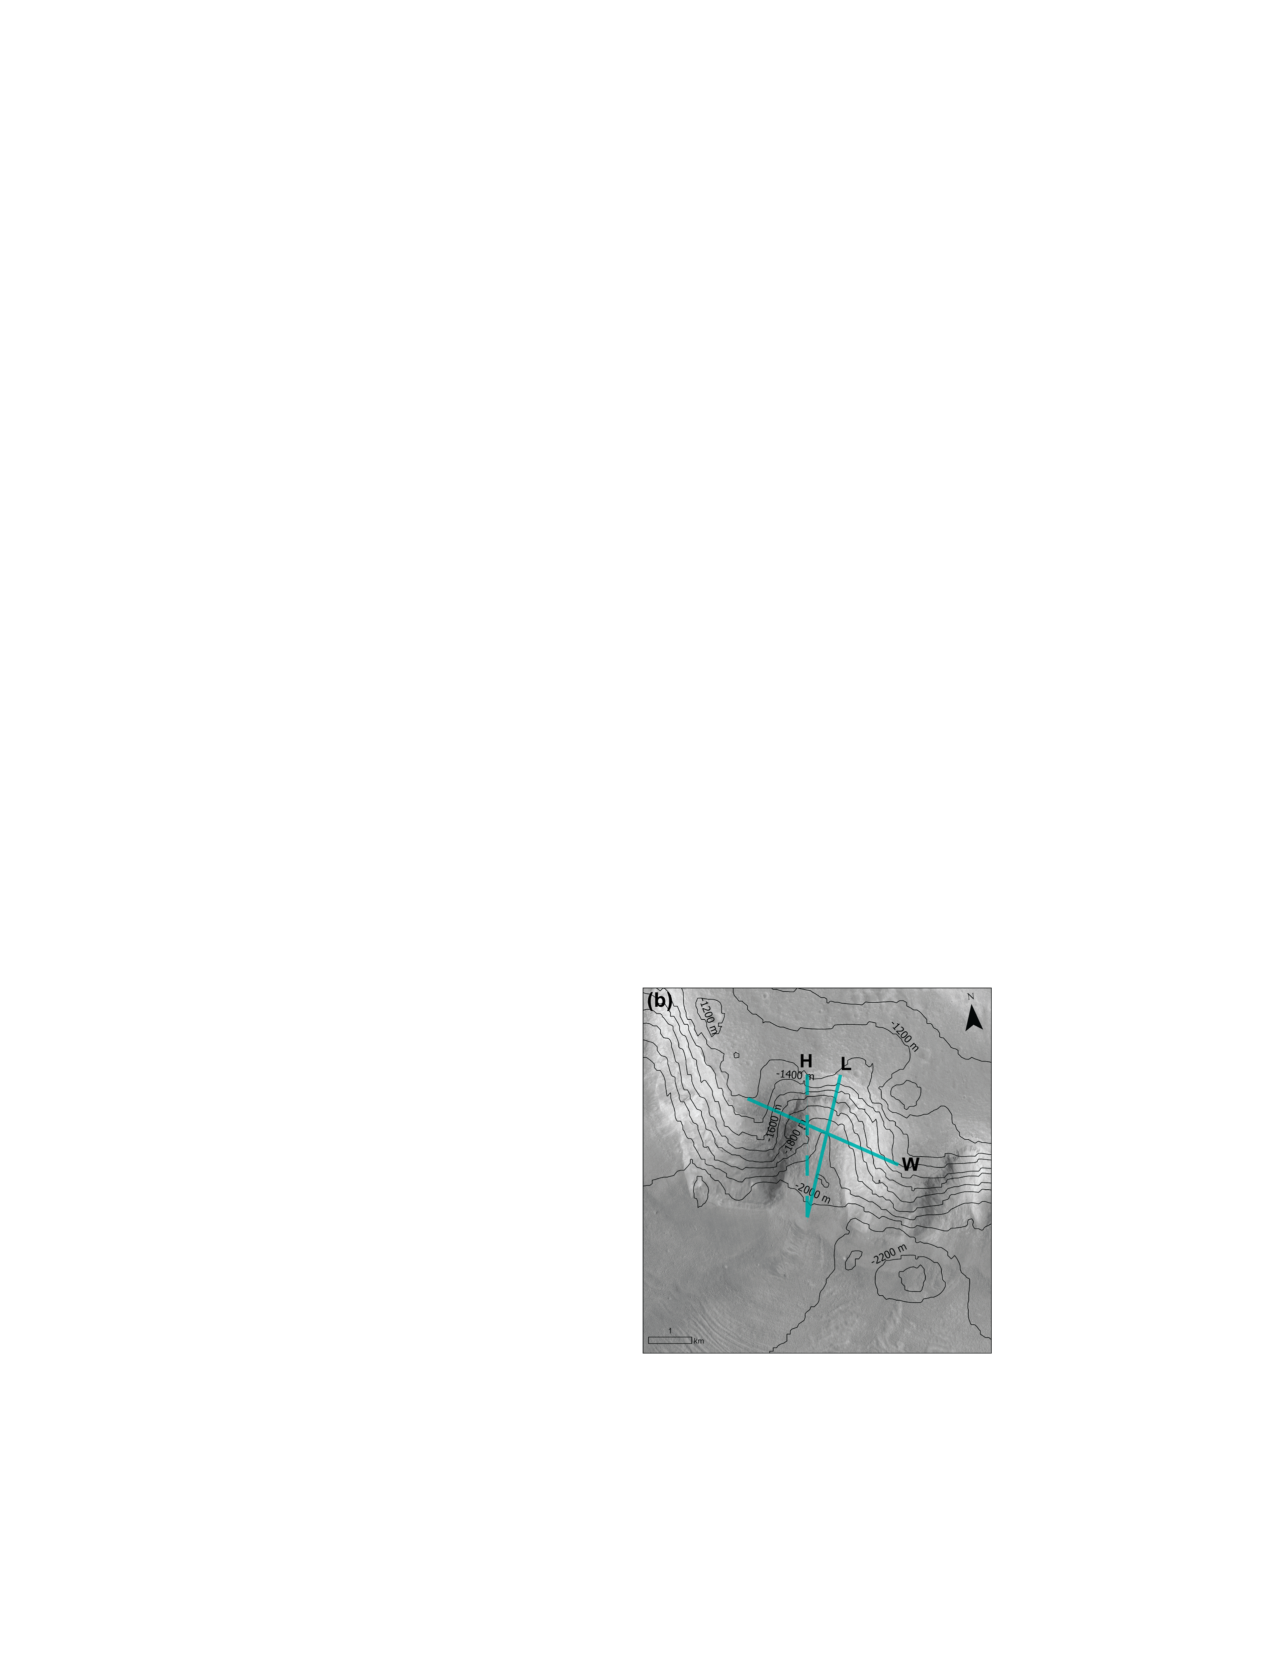
\includegraphics[
            width=\linewidth,
            height=0.6\textheight,
            keepaspectratio
        ]{Figures/Diagrams/Li26_Fig4b.pdf}
        \caption{Definitions of alcove dimensions (Figure from \cite{Li26}).}
        \end{figure}

    % \vspace{0.5em}

    % \scriptsize Alcove dimensions used by \cite{Li26}.
    \end{column}

    \end{columns}

\end{frame}

\section{Conclusions}

\begin{frame}{Main Findings}
    \begin{block}<+->{Evidence that...}
        \begin{itemize}
            \item<+-> Wet-based glaciation was active in Ismenius Cavus.
            \item<+-> Alcove glaciation occurred post-LVF/LDA.
            \item<+-> Sublimation-related features are young.
            \begin{itemize}
                \item Smooth
                \item Few craters
                \item Rubble
            \end{itemize}
        \end{itemize}
    \end{block}
\end{frame}
\begin{frame}{Implications}
    \begin{block}<+->{Geology}
        Wet-based glaciation
        \begin{itemize}
            \item Variable ice content of glacier with depth?
            \item Past geothermal activity?
        \end{itemize}
    \end{block}
    \begin{block}<+->{Climate}
        \begin{itemize}
            \item Alcove creates cooler conditions for stable ice?
            \item Past cooler climate (via $>30^{\circ}$ obliquity)?
        \end{itemize}
    \end{block}
\end{frame}

\begin{frame}{Future Work}
    \begin{block}<+->{Further data needed}
        \begin{itemize}
            \item<+-> Overlapping images $\rightarrow$ DEM analysis.
            \item<+-> Surface investigations to
            \begin{itemize}
                \item Confirm unit relationships.
                \item Confirm activity (or lack thereof).
            \end{itemize}
        \end{itemize}
    \end{block}
\end{frame}
\begin{frame}[allowframebreaks]{References} 
\printbibliography
\end{frame}
\frame{\titlepage}
\end{document}